\documentclass[a4paper,twoside,12pt]{book}


\usepackage[italian]{babel}
\usepackage[latin1]{inputenc}
\usepackage[dvips]{epsfig}
\DeclareGraphicsExtensions{.ps,.eps}
\usepackage{subfigure}
\usepackage[T1]{fontenc}

\usepackage{fancyhdr}
\usepackage{amsmath}
\usepackage{amssymb}
\usepackage{a4}
\newcommand{\clearemptydoublepage}{\newpage{\pagestyle{empty}\cleardoublepage}}
\newcommand{\nohyphens}{\hyphenpenalty=10000\exhyphenpenalty=10000\relax}

%% Layout della pagina
%\pagestyle{fancyplain}
%\setlength{\headheight}{14.5pt}
%\addtolength{\headwidth}{\marginparsep}
%\addtolength{\headwidth}{\marginparwidth}
%\renewcommand{\chaptermark}[1]{\markboth{#1}{}}
%\renewcommand{\sectionmark}[1]{\markright{\thesection\  #1}}
%\lhead[\fancyplain{}{\bfseries\thepage}]%
%      {\fancyplain{}{\bfseries\rightmark}}
%\rhead[\fancyplain{}{\bfseries\leftmark}]%
%      {\fancyplain{}{\bfseries\thepage}}
%\cfoot{}

% Questa lunghezza rappresenta la lunghezza completa della pagine, compreso
% lo spazio per le note a margine
%\newlength{\fullpagelen}
%\setlength{\fullpagelen}{\textwidth}
%\addtolength{\fullpagelen}{\marginparsep}
%\addtolength{\fullpagelen}{\marginparwidth}

\makeatletter
\renewenvironment{thebibliography}[1]
  {%
    \chapter*{\bibname}%
    \addcontentsline{toc}{chapter}{\bibname}%
    \@mkboth{\MakeUppercase\bibname}{\MakeUppercase\bibname}%
    \list{\@biblabel{\@arabic\c@enumiv}}%
    {%
      \settowidth\labelwidth{\@biblabel{#1}}%
      \leftmargin\labelwidth
      \advance\leftmargin\labelsep
      \@openbib@code
      \usecounter{enumiv}%
      \let\p@enumiv\@empty
      \renewcommand\theenumiv{\@arabic\c@enumiv}%
    }%
    \sloppy
    \clubpenalty4000
    \@clubpenalty \clubpenalty
    \widowpenalty4000%
    \sfcode`\.\@m%
  }%
  {%
    \def\@noitemerr
    {\@latex@warning{Empty `thebibliography' environment}}%
    \endlist%
  }   % Finisce qui la ridefinizione di thebibliography

\makeatother


\newcommand{\name}{$\mathcal{H}$eaven } 
\newcommand{\namens}{$\mathcal{H}$eaven} 
\begin{document}


\pagestyle{fancy}
\renewcommand{\chaptermark}[1]{\markboth{#1}{}}
\renewcommand{\sectionmark}[1]{\markright{\thesection\ #1}}
\fancyhf{} \fancyhead[LE,RO]{\bfseries\thepage}
\fancyhead[LO]{\bfseries\rightmark}
\fancyhead[RE]{\bfseries\leftmark}
\renewcommand{\headrulewidth}{0.5pt}
\renewcommand{\footrulewidth}{0pt}
 \fancypagestyle{plain}{
\fancyhead{}
\renewcommand{\headrulewidth}{0pt}}


%\thispagestyle{empty} \vspace*{\stretch{1}} \hfill\begin{minipage}[t]{.618\linewidth}
\flushright\itshape Dedicata a chi vi pare :-) .
\end{minipage}
\vspace*{\stretch{3}}
 \clearemptydoublepage
%\chapter*{{\em Ringraziamenti}}

\emph{ Ringraziate chi vi pare...}
\clearemptydoublepage
%\thispagestyle{empty}
\chapter*{Prefazione}

Blablabla
\clearemptydoublepage
\tableofcontents \clearemptydoublepage

%\chapter{Executive Summary}
\section{Vedi Paper} \clearemptydoublepage
%\section{Semantic Web}
\section{Stream Processing}
\section{Stream Reasoning}
\section{Empirical Research}

Tichy and collaborators [15] evaluated 400 articles published in 1993, 50 of them randomly selected papers published by ACM in 1993 and the rest systematically selected from a few journals in Systems and Software Engineering, and classified the research re- ported in the paper in five categories (quoting [15] definitions): \begin{itemize}
\item Formal theory: articles whose main contributions are formally tractable propositions, e.g., lemmata and theorems and their proofs.
\item Design and modelling: systems, techniques, or models, whose claimed properties cannot be proven formally. Examples include software tools, performance prediction models, and complex hardware and software systems of all kinds. The papers in this class were further classified in the categories 0\%, 0–10\%, 10– 20\%, 20–50\, and +50\%, according to the proportion of the paper that was dedicated to the evaluation of the new system, technique, or model.
\item Empirical work: articles that collect, analyse, and interpret observations about known designs, systems, or models, or about abstract theories or subjects (as this paper does). The emphasis is on evaluation, not on new designs or models.
\item Hypothesis testing: articles that define hypotheses and describe experiments to test them.
\item Others: articles that do not fit any of the four categories above, e.g., surveys.
\end{itemize}

\subsection{Software Testing}
\subsubsection{SOAK}
\subsubsection{Stress}

\section{Benchmarks}
\subsection{TCP}  \label{sec:tcp}


\subsection{Reasoning Benchmark}
\subsubsection{LUBM}
\subsection{DBMS \& CEP Benchmarking}
\subsubsection{Linear Road}
\subsection{Stream Reasoning Benchmark}
\subsubsection{SRBench}
SRBench [5] proposes a suite of test queries and defines metrics to evaluate the
performance of the system. This benchmark contains 17 queries to gather the
properties of the RDF stream engines. The queries vary to ensure that several
features of the target system are tested: queries involving single or multiple input
streams, queries over stream-only data sources or over mixed stream and static
data source, etc. In [5] the authors applied the benchmark on the existent RDF
stream engines, and explained the differences in term of supported functionalities.
Time and memory performance tests, and scalability tests are not targeted
in the actual version of SRBench.
\subsubsection{LSBench}
LSBench [6] proposes three tests to evaluate the RDF stream engines. The
first one is a functional test to verify the operators and the functionalities supported
by the engines: it is a test similar to the one proposed by SRBench. The
second test is a correctness test: its goal is to verify if the tested RDF stream
engine produces the correct output. Actually this analyses only the number of
produced answers, assuming that the contents of the output are correct. Finally,
the third test is a maximum input throughput test: it has the goal evaluate the
maximum throughput of the RDF stream engines. This test is done increasing
the rate of data in the stream and verifying the number of the answers. For each
test a set of 12 queries is provided; similarly to SRBench, the queries vary to
take into account different features of the engines (single and multiple streams,
presence of static data, etc)

\subsubsection{Correttezza}
\subsubsection{Seven Commandaments}

 \clearemptydoublepage
In this Chapter we introduce the work this thesis involved. First we introduce the motivations behind this research. In Section \ref{sec:comparative-research} we describe the themes that have inspired this survey towards the Comparative Research and, as a conclusion, we formulate our research question. Then, in Section \ref{sec:requirements} we formalise the requirements we have to satisfy in order to successfully answer the research question.

\section{Comparative Research}\label{sec:comparative-research}
The Computer Science (CS) community classifies its activity in many works and shows that its research mostly follow an engineering epistemology \cite{Wainer:2009:EEC:1518331.1518552,Tichy:1995:EEC:209090.209093}. A majority of publications belongs to \textit{empirical work} and \textit{design \& modelling} classes of Tichy's taxonomy (See \ref{sec:tcp} ) and, among them, proposals of new systems or models  are more common then the evaluations of existing ones. This contrasts with other engineering areas, where the experimental research is almost dominant. CS needs to focus on collecting, analysing, and interpreting the observations of those works it usually only designs or implements. Now the question is: \textit{What are the motivation under this CS research lack?} The main problem in evaluating software systems or models regards their complex and multifaceted nature. Other explanations concern the difficulties of conducting realistic evaluations, because of the number of the involved variables.

A Systematic Comparative Research Approach (SCRA) is typically used in those research fields where the complexity of its research subjects goes beyond the possible observable models. This is the case of the social sciences, which exploit techniques to deal with complex cases that can not be simplified in experimental setting. The analysis of a single case study allows to deeply understand it, but it makes difficult to engage any form of generalisation. On the other hand, cross-case studies are more relevant and allow general thinking, but their final complexity represents a problem. We need a strategy that reduces the analysis complexity without lose the relevance of each involved system. In this regard, Russel Schutt discusses four stages to systematic qualitative comparative studies for history social phenomena:
\begin{enumerate}
\item[S.1] Premise of the investigation: identification of possible causes.
\item[S.2] Choose the cases to examine (location, language, gender).
\item[S.3] Examine the similarities and the differences with shared methods.
\item[S.4] Propose a causal explanation for the phenomena.
\end{enumerate} We will return on these stages later. Is important to understand that this investigation method becomes meaningful inside the experimental environment. An \textit{experiment} is a test under controlled conditions that is made to demonstrate a known truth or examine the validity of an hypothesis (W.R Inge). Complex cases are seen as a combination of known properties upon which is possible to identify parallelism or state contrasts and are used to set up experiment configuration. Researcher can exploit the notions of \textit{reproducibility} to appreciate variations on changing experiment conditions, \textit{repeatability} to consolidate observations trough multiple identical executions and \textit{comparability} to contrast the results to identify the differences.

Some Computer Science sub-fields attempt to lead Case-driven analysis by the notion of experiment. Database community explores the idea of comparative research trough benchmarking techniques and actually the quality of empirical studies is rising \cite{Wainer:2009:EEC:1518331.1518552}. It is worth to note Jim Gray's work about transactional benchmarking (TCP, Section \ref{sec:tcp}) and Domain Specific Benchmarks (DSB). He states that \textit{any comparison on performances starts with the definition of a benchmark or a workload}, but we need know the relevance of the metrics. Measurement variations are very frequent from one application to another, because each system is thought to solve a small problems set. A DSB must response properly to system diversities, by specifying a synthetic workload to describe typical applications in the problem domain; moreover it must provide workload performances on various systems and an estimation of relative performance on the problem domain.
Gray proposes also four criteria that a DSB must meet, which are:
\begin{enumerate}
\item[G.1] \textsc{Relevance}, it must measure the performance peak of systems when
performing domain typical operations.
\item[G.2] \textsc{Portability}, it must be easy-to-implement on many different systems and architectures
\item[G.3] \textsc{Scalability}, it must be meaningful for both small and large computer systems
\item[G.4] \textsc{Simplicity}, it must be understandable to obtain credibility
\end{enumerate} 

Let's consider the relation between this criteria and Schutt's stages presented above. Gray states G.1 to identify the relevant metrics for the evaluation, as Schutt does in his first stage (S.1), which demands a pre-analysis phase of the phenomenon. Moreover, Social Science does not care about problem scaling, because those properties that define the case also determine the problem dimension (S.2). Gray poses the same concept in the DB context with G.2, demanding implementation-related conditions, but it also explicit the need to consider the dimension-related issues in G.3, because DB must consider the scaling problem. Last but not least, G.4 demands simplicity to obtain credibility while S.3 suggests to exploit those evaluation methods that are commonly accepted (shared) by the research community. 

Motivated by the growing number of RDF Stream Processing techniques, the Stream Reasoning (SR) community strongly calls of evaluation practices to allow comparison on them. RSP Engines, the systems that implement this techniques, have an high resulting complexity (Further details in Section \ref{sec:sfp}). The execution mechanism they implement together with their execution semantic and the environment where this execution happens are evaluation-related characteristics, which demonstrate that a meaningful comparison between RSP Engines is non-trivial. Chapter 	\ref{chap:evaluation} shows in details that may be difficult to analyse those system, even in case of simple and well defined architectures. 
The interest on cross-case analysis between complex subjects draw the need of a comparative research approach. Initial efforts in this direction try to define frameworks that resume  DSMSs \cite{arasu2004linear} and Reasoning \cite{Guo2005} benchmarking studies. LS Bench and SR Bench propose a set of queries, data sets, and methods to test and compare existing RSP engines (see Section\ref{sec:sr-benchmarking}). Both these works share a common background: the Linear Road Benchmark (LRB) is the only existing benchmark for relational data stream processing engines. Actually LRB only states which requirements a benchmarked DSMS must satisfy, without proposing a concrete solution. LS Bench and SR Bench implement and extend this work, but they do not re-contextualise this requirements in SR context. Following discussions identify other lacks, i.e none of them completely face the problem of evaluating query result correctness, because they do not analyse engine semantics. LS Bench concentrates attention to the evaluation of engines throughput and it checks the correctness of the query result measuring the mismatch after comparing different RSP Engines. SR Bench entirely ignores this issue and analyses the coverage of SPARQL constructs for each commercial engine. More recent works describe deeply all the RSP Engine properties, identify the future challenges and provide a standardization benchmarking requirements: commandments for a meaningful testing on RSP Engines\cite{DBLP:conf/esws/ScharrenbachUMVB13}.

Stream Reasoning community still lacks an infrastructure that can control the execution environment and allow to systematic testing. LRB provides a simulator to validate the benchmarked DSMS systems, but does not face the problem of an online evaluation it. Researches in this area demonstrates that RSPEngine execution semantic is relevant \cite{Botan:2010:SMA:1920841.1920874}, but does not evaluate its cost. From the aerospace engineering we borrow the idea of an \textit{Engine Test Stand}, a tool that allows experiments design, their systematic execution and automatic results comparison. An engine can not be evaluated only by an architectural viewpoint, it is necessary to understand it behaviour during the execution: \textit{A process cannot be understood by stopping it. Understanding must move with the flow of the process, must join it and flow with it}\footnote{The First Law of Mentat, quoted by Paul Atreides to Reverend Mother Gaius Helen Mohiam}. Thus, the community questioned itself \textit{How to support SRCA on RSP Engines}? Now we have queries, dataset and methods, that partially answer it and the new research question is "\textit{Can an engine test stand, together with queries, datasets and methods, support SCRA for Stream Reasoning?}". The next section poses the requirements a proper answer to this research question must satisfy.

\section{Requirements} \label{sec:requirements}

In order to simplify and support Systematic Comparative Research Approach on RSP engines trough an Engine Test Stand we need to answer the following questions: 
\begin{enumerate}
\item[Q.1] How can the behaviour of system be evaluated? 
\item[Q.2] What makes this evaluation rigorous? 
\item[Q.3] How can this rigorous evaluation be automated?
\end{enumerate} To answer Question Q.1 we exploit traditional definition of \textit{experiment} presented above. We answer Q.2 referring to \textit{reproducibility}, \textit{repeatability}, and \textit{comparability} of experiments. Trough this concepts it is easy to answer Q.3 formalising the requirements for the solution.

\textit{Reproducibility} refers to measurement variations on a subject under changing conditions. We gather this conditions into experiment configuration, whose specification is up to the user. For this reason the solution must be independent from:
\begin{enumerate}
\item[R.1] \textit{Test data}, relevant RDF data streams and ontologies chosen from user domain of interest. %R.2.1
\item[R.2] \textit{Query}, relevant queries registered from user domain of interest.
%thus allowing users to register relevant queries from their domains of interest. %R.2.2
\item[R.3] \textit{Engine}, any RSP Engine tested by the means of easy-to-implement software interfaces. 
%thus allowing users to put an RSP engine on the test stand by the means of easy to implement software interfaces, e.g., it should adopt an event-base architecture as normally done by RSP engines and present events to RSP engine in a simple to parse RDF serialisation. %R4 e R5
\end{enumerate}

\textit{Repeatability} refers to variations on repeated measurements on a subject under identical conditions. The solution must not affect the RSP engine evaluation, which, from a practical point of view, poses two requirements:
\begin{enumerate}
\item[R.4] it must not be running when the RSP engine is under execution. %R.1.2
\item[R.5] it must have reduced (and possibly constant) memory footprint. %R.1.1
\end{enumerate}

\textit{Comparability} refers to performance measurements nature and the relations between experimental conditions. The SCRA demands both the definition of \textit{comparable metrics} and the standardization of \textit{evaluation methods}, which means the solution must:
\begin{enumerate}
\item[R.6] include \textit{basic set of performance measurements} \cite{DBLP:conf/esws/ScharrenbachUMVB13}.
\item[R.7] enable users extensions with new software sensors and specific measurements collection.
%\item[R.7] enable users software extensionsa and specific measurements collection.
\item[R.8] support performance measurements collection for further analysis.
\item[R.9] allow \textit{qualitative analysis} trough tools for result visualization
\end{enumerate}


In terms of software engineering, any solution which satisfies the requirements above demands also some technical ones: 
\begin{enumerate}
\item[R.10] \textit{Extendible Design}, the possibility to replace theoretically each module with one with the same interfaces, but different behaviour, without affecting architecture stability.
\item[R.11] \textit{Event-base architecture} to properly communicate with  RSP Engines, which normally exploit it.
\item[R.12] \textit{Easy-to-Parse RDF Serialisation} for the events presented to the RSP Engine in exam
\end{enumerate}

SCRA is case-oriented, it needs \textit{successful analysis and evaluations examples} to pose experimental guidelines and \textit{initial terms of comparison}. We call baseline an elementary solution for the RSP problem, which is relevant from an experimental viewpoint. To fulfil this request the answer to our research question must consider to have specific baseline modules and satisfy their own requirements, which are: \begin{enumerate}
%\item[R.13] Be a Solution: it solves the problem entirely, without concerning about performance. % devono risolvere interamente il problema, nel nostro caso devono essere complete e sound rispetto ad entailment regime che si è scelto
\item[R.13] It must be Elementary: requiring the minimum design effort, which means be a naive solution and do not care about performances.  % non devono essere soluzioni smart, devono chiedere il minimo effort
\item[R.14] It must be Eligible: being a fair term of comparison w.r.t. commercial solutions. %e' inutile se sono sopra un'ordine di grandezzaad esempio in latenza, rispetto ad una soluzione commerciale. probabilmente è sbagliata la domanda di ricerca
\item[R.15] It must be Relevant: covering one of the theoretical solutions. %la soluzione che coprono deve essere una delle immediate soluzioni del problema iniziale: Graph vs Statement o Inc vs Naive, tempo controllato esternamente, ecc
\item[R.16] It must be Simple: allowing to identify easily those characteristics which support hypothesis formulation and comparison.  %non devono offrire api più complesse rispetto a un RSPEngine tradizion	ale.
\end{enumerate}

%Some of those requirements assume a problem-specific meaning. As advocated in the early works on Stream Reasoning \cite{1,2} the most simple approach to create a stream reasoning system is arrange into a pipeline DSMS with a reasoner. Baselines design must follow this statement to develop a full solution [R.13] which is very simple w.r.t the commercial ones presented in Chapter 2 [R.14]. Chapter 2 also states how two main design decisions can distinguish the baselines: the RDF stream model and the architecture. From this point of view the solution must provide at least four Baselines [R.16], which cover all possible combinations those design choices.
 \clearemptydoublepage
%In this chapter we present  \namens,  an open source framework for Systematic Comparative Research on RSP Engine.
It consists in four baselines and two main components: the Test Stand and the Analyser. Firstly, Section \ref{sec:teststand} introduces the Test Stand, which satisfies requirements from R.1 to R.8 and from R.10 to R.12, by executing experiments on an RSP Engine. Section \ref{sec:baselines} describes the Baselines, four RSP Engines that are included in \name as naive terms of comparison, since they fulfil requirements R.13 and R.14. Finally, Section \ref{sec:analyser} presents the Analyser, which addresses requirements R.9 and R.10  allowing the user to visualise, investigate and compare experiment results. %Soundness and completes of the query answering process are assessed post-hoc by comparing the results of an RSP engine with a term of comparison whose results are correct (see Section 5).

\section{Test Stand}\label{sec:teststand}

Aerospace engineering defines an engine test stand as a facility used to develop, study and characterise engines. It allows to test operating regimes and offers measurement of several variables associated with engine process. A test stand may uses actuators for attaining a specific engine state, which is a unique combination of the engine properties. The information collected through the sensors depends on the engine manufacturer, which usually provides his own stand or the facilities to test the engine with commercial solutions. The test stand executes black box testing over engines, because its users can not rely to known engine internal mechanisms.

The definition above still holds its relevance in the SR context, with the difference that engines subject of the testing, RSP Engines, are IO-Systems. An RSP Engine consumes an RDF Stream and  produces a new one, by applying queries under some entailment regime and w.r.t. an ontology which does not change over time. Describing an RSP Engine means understanding the relation between input stream, the queries registered to it and what we call \textit{operational semantics}, which requires to know the RSP Engine internal processes. Indeed, black box testing is the only possibility to analyse such system with a test stand. Even having access to the entire RSP Engine code, may results hard to characterise all the RSP Engine properties a priori. 

Figure \ref{fig:architecture} shows \name \textsc{Test Stand} design. It contains the block schema of the modules that composes the \textsc{Test Stand} pipeline. Moreover, we enumerates in the Figure the events that pass trough the the \textsc{Test Stand} while it is executing and experiment. In the following subsection we describe each elements that Figure \ref{fig:architecture} summarises. In Subsection \ref{sec:modules} we describe the \textsc{Test Stand} pipeline and each module that composes it, in Subsection \ref{sec:test-stand-data-model} we detail the Data Model exploited to represent experiments, events, query results and measurements. Finally, in Subsection \ref{sec:test-stand-workflow} we describe the \textsc{Test Stand} workflow, how it executes experiments to stress the RSP Engine we want to test.

\begin{figure}[tbh]
\centering
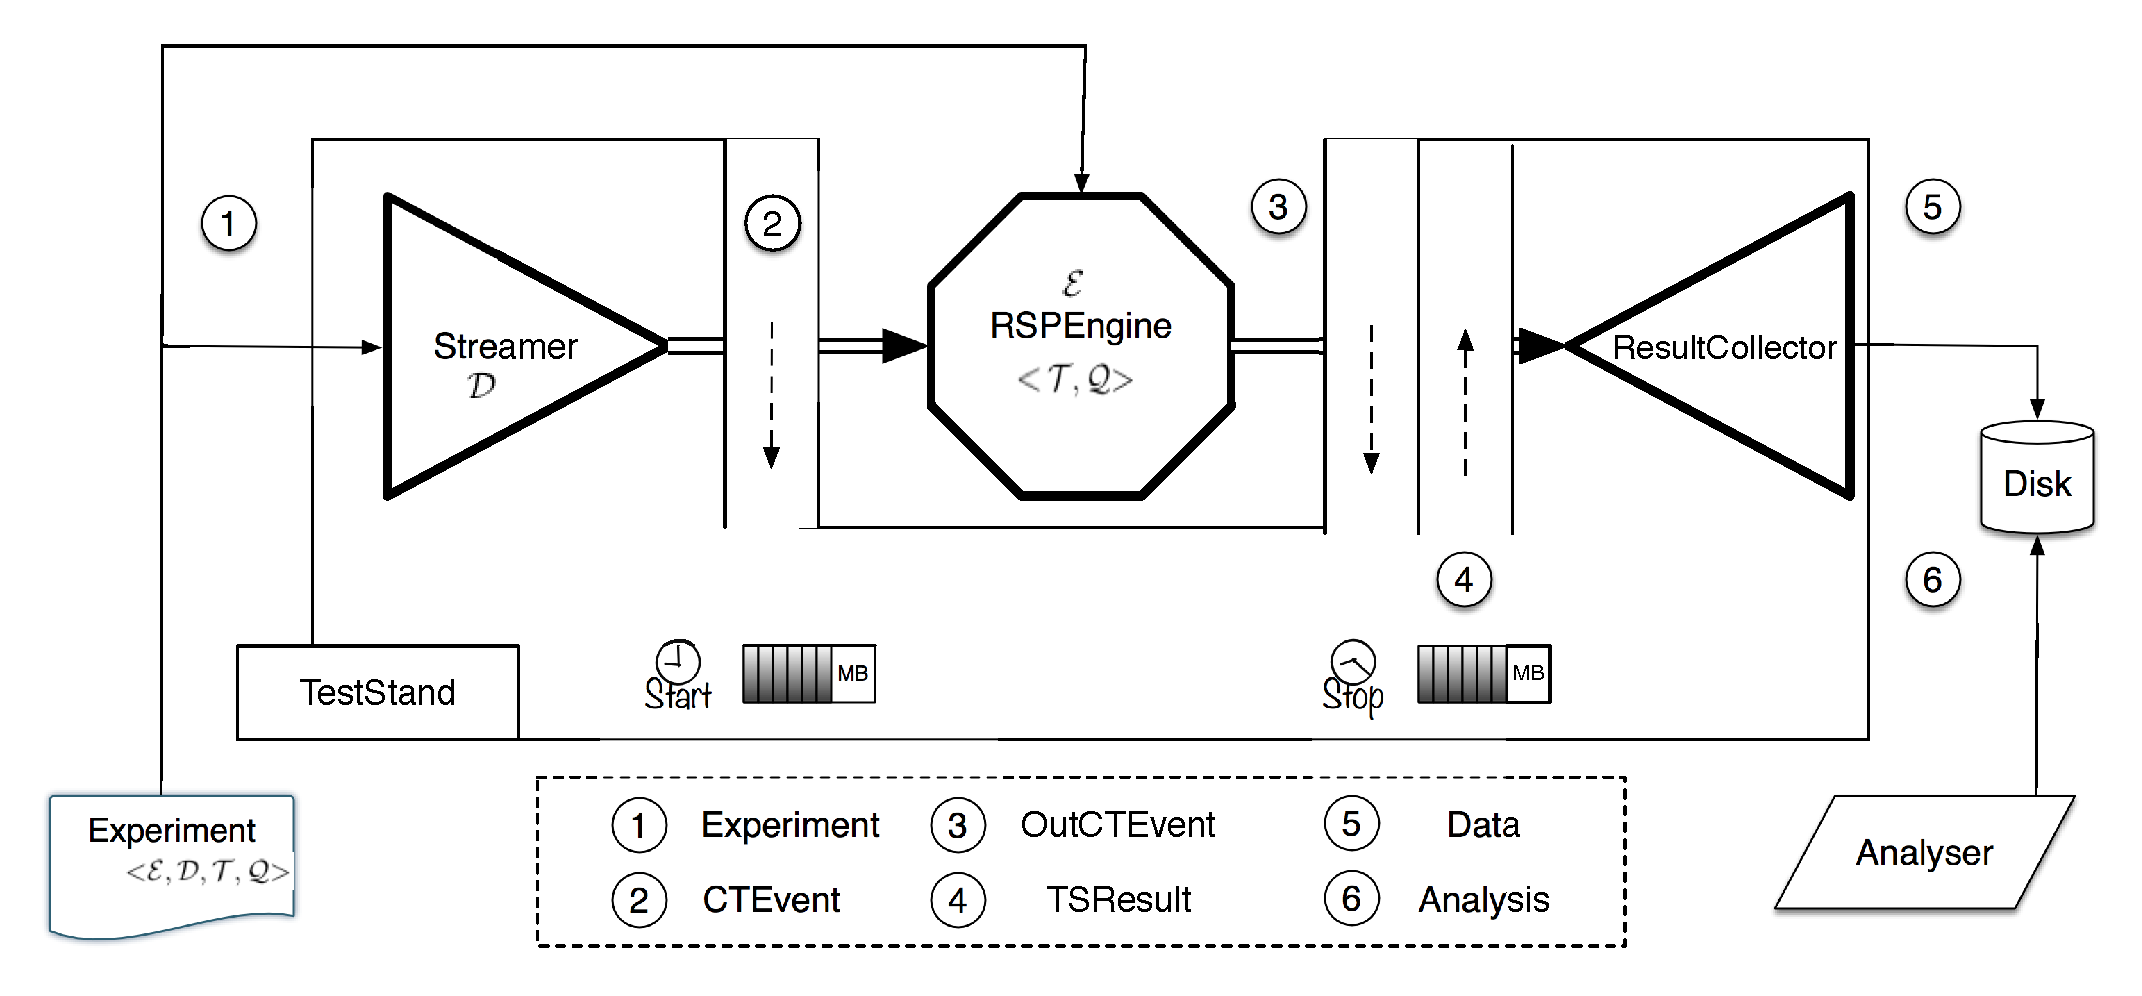
\includegraphics[scale=0.37]{images/schema2}
\caption{\name modules and workflow} 
\label{fig:architecture}
\end{figure}


\subsection{Modules}\label{sec:modules}

\noindent An aerospace test stand exploits different modules to simulate the operating regime for the engine in use ( i.e a module for fuel distribution, one for the engine mechanic support or to enable users interaction during the execution ). Modularity allows to extend the test stand and specify testing procedure. 

We design \name \textsc{Test Stand} as modular system for the same reasons, guaranteeing modularity [R.10]. Thus, it consists into the following three stand-alone modules:
\begin{itemize}
\item the \textsc{Streamer}, a source for the input RDF Stream
\item the RSP Engine we want to test;
\item the \textsc{Result Collector}, a data acquisition system for both the query results and the gathered measurements.
\end{itemize}

\noindent The architecture of \name \textsc{Test Stand} is represented in Figure \ref{fig:architecture}. The \textsc{Test Stand} modules  are arranged into a pipeline and communicates exchanging events [R.11]. Their interfaces allow each of them to be replaceable with an other ones with a different behaviour, but which complies with the interfaces specifications.

The execution starts with the \textsc{Streamer}, which hides the data generation logic in order to obtain data independence [R.1]. It pushes an RDF Stream directly to the mounted RSP Engine. It is up to the \textsc{Streamer} to respect [R.5] and not to influence the memory footprint with heavy data loading tasks. 

An interface adapts the event flow to the RSP Engine in use, fulfilling [R.2] (Engine Independence) and hiding the query registration process [R.3] (Query independence), which happens at engine level and is up to the RSP Engine provider.

The \textsc{Result Collector} is at the tail of the pipeline. It is part of the \textsc{Test Stand} because the performance measurements are processed and gathered during the execution, together with the queries results data. The \textsc{Result Collector} is responsible to save all this data at the end of each cycle, without influencing the system. The evaluation usually happens a-posteriori trough the Analyser (Section \ref{sec:analyser}). However, real time analysis of the performance measurements are possible, but they may violate some requirements like [R.4] and [R.5]. 

Last but not least, the Test Stand has an external structure that sustains other modules and can be considered as a module itself. It allows the user to control the process through accessible APIs. It gathers the data sampled by the sensors during the execution and adds them to the query results. The \textit{Test Stand} External Structure allows the user (the RSP Engine developer) to develop a specific testing procedure for a given engine. The measure set extensions are possible by adding user defined metrics, according to requirements [R.7] and [R.10]. Finally, it controls the process ensuring that the \textsc{Test Stand} does not run when the RSP Engine run as required by [R.4].

\subsection{Experiment \& Data Model}\label{sec:test-stand-data-model}

\noindent The Test Stand accepts as input an \textsc{Experiment} in the form of a tuple \\ $<\mathcal{E},\mathcal{D},\mathcal{T},\mathcal{Q},>$ where:
\begin{itemize}
\item $\mathcal{E}$ is the RSP Engine subject of the evaluation (satisfying requirement [R.3]); 
\item $\mathcal{D}$ is the input dataset [R.1]; 
\item $\mathcal{T}$ is the ontology [R.1]; 
\item $\mathcal{Q}$ is the query to be continuously answered by $\mathcal{E}$ [R.2]. 
\end{itemize}

From an experimental point of view, which metrics we sample during the execution have a different influence on the measurements. For example, asking to the system for the memory usage may influence the latency calculus or saving on disk the query results may influence the memory footprint. Thus, we define there main kinds of experiment, distinguishing on the data we want to sample and save. Notice that which experiment kind choose depends on the goal and the error tolerance of the research.

\begin{itemize}
\item Latency Experiment, where only the latency is calculated and no query result is saved on file
\item Memory Experiment, where only the memory is gathered and no query result is saved on file
\item Query Experiment, where query results are saved on file.
\item Any combination of the previous experiment types.
\end{itemize}


\noindent In order to describe the Data Model exploited by the \textsc{Test Stand}, we draw the Entity-Relation diagram in figure \ref{fig:er}. The diagram does not include entity attributes to simplify the interpretation, but they are reported in the following Logic Schema:
\begin{figure}[tbh]
  \centering
	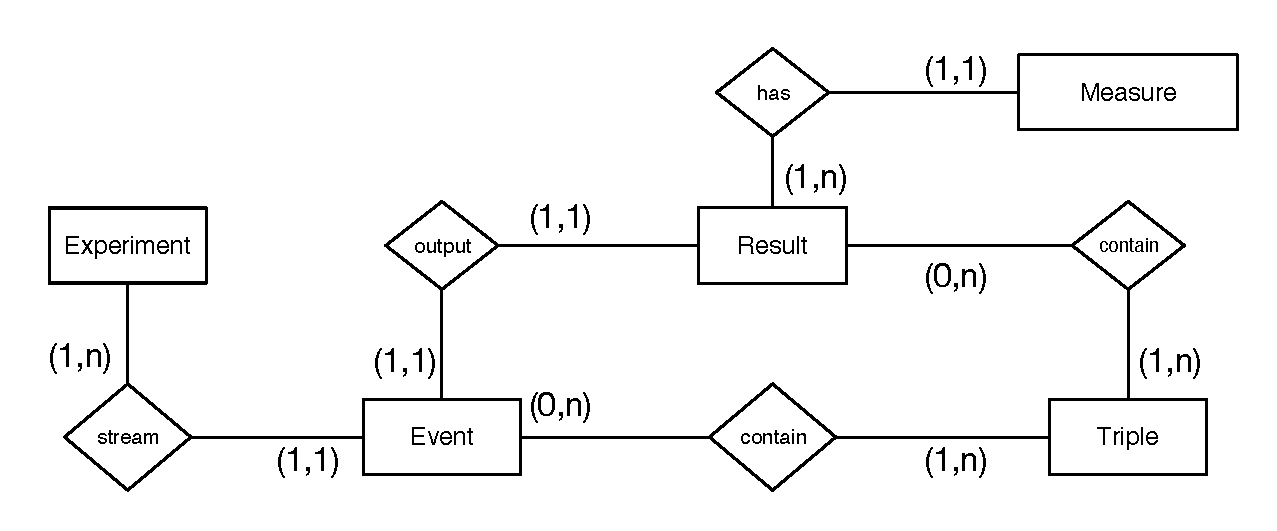
\includegraphics[width=\linewidth]{images/er-db}
	\caption{ER-Diagram \name data} 
  	\label{fig:er}
\end{figure}\\
\noindent\textsc{Experiment}(\underline{ID}, Timestamp Start, Timestamp End, Engine, Ontology, Query, Dataset, Description)\\
\textsc{Event}(\underline{ID, Experiment ID}, Timestamp)\\
\textsc{Result}(\underline{Result ID, Experiment ID}, Event ID)\\
\textsc{Measure}(\underline{ID}, Value)\\
\textsc{Measurement Set}(\underline{Measure ID, Result ID, Experiment ID})\\
\textsc{Triple}(\underline{S,P,O})\\
\textsc{Output Triple}(\underline{Result ID, Experiment ID, S, P, O})\\
\textsc{Input Triple}(\underline{Event ID, Experiment ID, S, P, O})\\

The \textsc{Experiment} entity contains the metadata of the tuple $<\mathcal{E},\mathcal{D},\mathcal{T},\mathcal{Q},>$, which semantic is explained above. "Timestamp Start" and "Timestamp End" are relevant metrics for further analysis and system control. 

The \textsc{Event} is unique inside an \textsc{Experiment}, it is possible to send two events with the same timestamp and identical tripleset. The Timestamp field allows to order events after the execution

The \textsc{Result} is associated with one and only one \textsc{Event}. It contains the results to the engine queries w.r.t the active window and the set of the measure gathered during the execution. 

The \textsc{Measurement Set} table represents the many-to-many relation between the \textsc{Result} and a number of measure that may variate  to fulfil requirement [R.7] (extendible measurement set). 

We include the concept of the \textsc{Triple} in order to model the content of \textsc{Event} and \textsc{Result}. \textsc{Input Triple} and \textsc{Output Triple} are the tables which represent two many-to-many relations, respectively between \textsc{Triple} and \textsc{Event} and \textsc{Triple}  and \textsc{Result}

\subsection{Test Stand Workflow}\label{sec:test-stand-workflow}

\noindent The \textsc{Test Stand} orchestrates the communication between the upstanding models, forcing the \textsc{Streamer} to push events to the RSP Engine and the \textsc{Result Collector} to listen the output and collect the results. To explain the \textsc{Test Stand} workflow we split the process at the points when the modules exchange events. Indeed, each message represents a different logic step in the experiment execution cycle.

Six different steps are identified by six events exchanged by \textsc{Test Stand}, \textsc{Streamer} and RSP Engine. The \textsc{Result Collector} only receives events, terminating each cycle.

In step (1) the \textsc{Test Stand} takes the experiment and starts the execution. It executes the experiment $<\mathcal{E},\mathcal{D},\mathcal{T},\mathcal{Q},>$ stressing $\mathcal{E}$ for a certain period of time looping through the steps from (2) to (5) illustrated in Figure \ref{fig:architecture}.                                                                                                                                                                                                                                                                                                                                                                                                                                                                                                                                                                                                                                                                                                                                                                                                                                                                                                                                                                                                                                                                                                                                                                                                                                                                                                                                                                                                                                                                                                                                                                                                                                                                                                                                                                                                                                                                                                                                                                                                                                                                                                                                                                                                                                                                                                                                                                                                                                                                                                                                                                                                                                                                                                                                                                                                                                                                                                                                                                                                                                                                                                                                                                                                                                                                                                                                                                                                                                                                                                                                                                                                                                                                                                                                                                                                                                                                                                                                                                                                                                                                                                                                                                                                                                                                                                                                                                                                      

In step (2), the \textsc{Streamer} pushes to $\mathcal{E}$ an event \textsc{CTEvent}. This event is a portion of an RDF Stream picked from the data $\mathcal{D}$ and it consists of a set of RDF triples with the same timestamp. In order to satisfy [R.12], it sends triple in N-Triple\footnote{\url{http://www.w3.org/2001/sw/RDFCore/ntriples/}}, which is the easiest RDF serialisation to parse.  


In step (3) $\mathcal{E}$ pushes to the \textsc{Result Collector} an event \textsc{OutCTEvent}. It contains the current answer to the query $\mathcal{Q}$ registered in $\mathcal{E}$ given the ontology $\mathcal{T}$. The \textsc{Test Stand} expects $\mathcal{E}$ to output result in N-Triple format. 

Notably, to place any RSP engine on the \textsc{Test Stand} (requirement [R.3]) \name provides a simple software wrapper that, when it receives a \textsc{CTEvent}, adapts it to the RSP engine specific format, pushes it in the RSP engine, and listens to the RSP engine output so to transform such an output in a \textsc{OutCTEvent}.

To measure performances (requirement [R.6]) the \textsc{Test Stand} performs several actions both before step (2) and after step (3) to collect data from the sensors. Previous works about Stream reasoning \cite{DBLP:conf/esws/ScharrenbachUMVB13} shows that the minimal performance measure set includes \textbf{Latency} -- defined as the delay between the injection of an event in the RSP engine and its response to it --, \textbf{Memory Load} -- defined as the difference between total system memory and the free one --, and \textbf{Completeness \& Soundness} of query-answering results. To measure latency, it starts a timer before (2) and stops it after (3). To measure memory load, it asks for the free memory of the system after step (3). Completeness \& Soundness are evaluated with post-processing analysis of the query results data.

In step (4), those observations are added to the outputs of $\mathcal{E}$ as annotations and are pushed to the \textsc{Result Collector}.  We name \textsc{TSResult} the event that contains the sensor data plus the query results produced by the engine.  

The \textsc{Test Stand} works in a single thread mode, blocking the execution of its components when it performs the measurements in (2) and (3) [R.4].  

In step (5) the \textsc{Result Collector} saves \textsc{TSResult} for post process analysis [R.9], executed trough the \textsc{Analyzer}. It does so saving the content of any TSResult  [R.8].

\section{Baselines}\label{sec:baselines}

\noindent In Chapter \ref{chap:problem-settings} we state that a Systematic Comparative Research Approach needs initial terms of comparison to lead the investigation. \name contains a set simple and easy-to-use RSP Engines called "Baselines". As the name lets to guess, these engine fulfil the four characteristics, detailed in Section \ref{sec:requirements}, required by an RSP Engine to be classified as a baseline inside the SR research field. Thus, \name Baselines are \textit{Elementary}, \textit{Relevant}, \textit{Simple} and \textit{Eligible}. developed to fulfil this lack. 

%We exploit them to define some qualitative methods of investigation and to prove the usability of the Test Stand. 
Early works on SR \cite{DBLP:conf/fis/ValleCBBC08,Walavalkar08streamingknowledge} describe the most simple approach to create a stream reasoning system: pipelining a DSMS with a reasoner. The DSMS is responsible to handle the data stream, moving from infinite sequences to finite (and processable) sets of events. The reasoner instead applies SPARQL queries on this set of events, exploiting its reasoning capabilities over a context that can be considered as static, but remains continuous. We focus on RDF Stream Processing, whose foundations, as explained in Section \ref{sec:sfp}, are: 
\begin{enumerate}
\item[1.] RDF streams, detailed in Section \ref{sec:rdfstream}
\item[2.] An extensions of SPARQL to manage continuous data (see Section \ref{sec:continuous-sparql}
\item[3.] reasoning algorithms
\end{enumerate}

\begin{figure}[tbh]
 \centering
\subfigure[Baseline A: Naive]{
	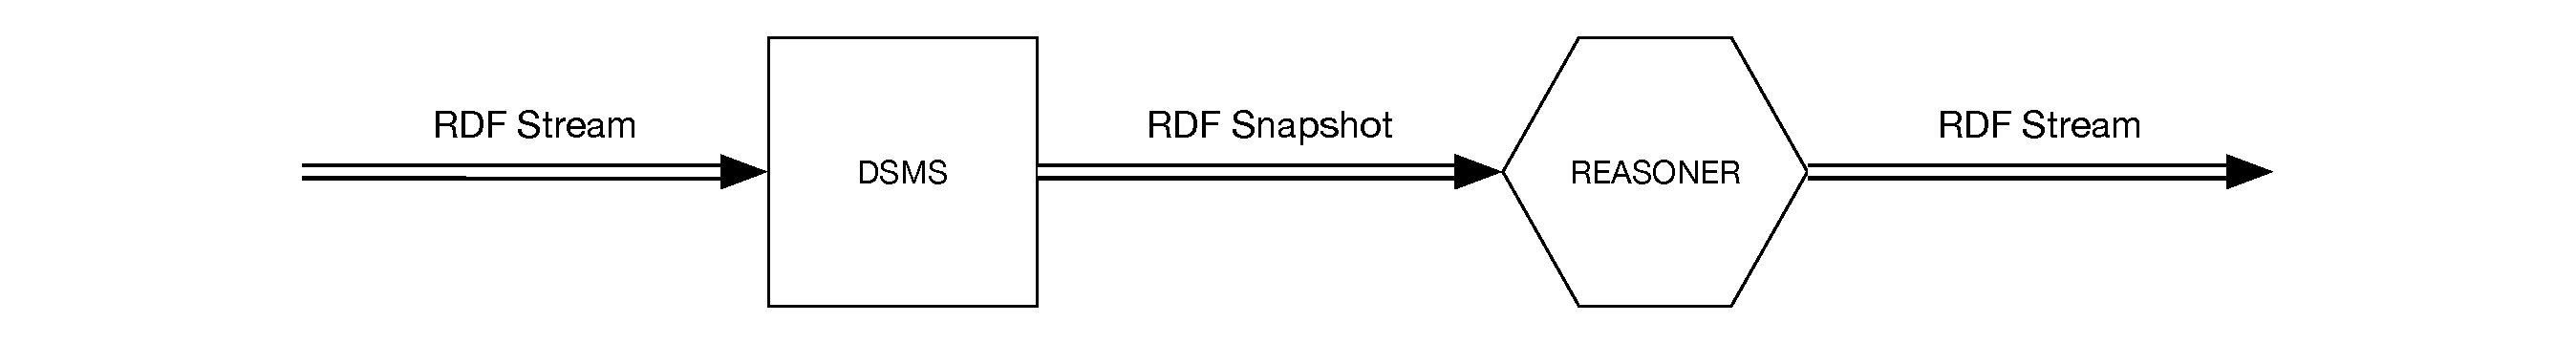
\includegraphics[width=\linewidth]{images/baseline-a}
}
\subfigure[Baseline B: Incremental]{
	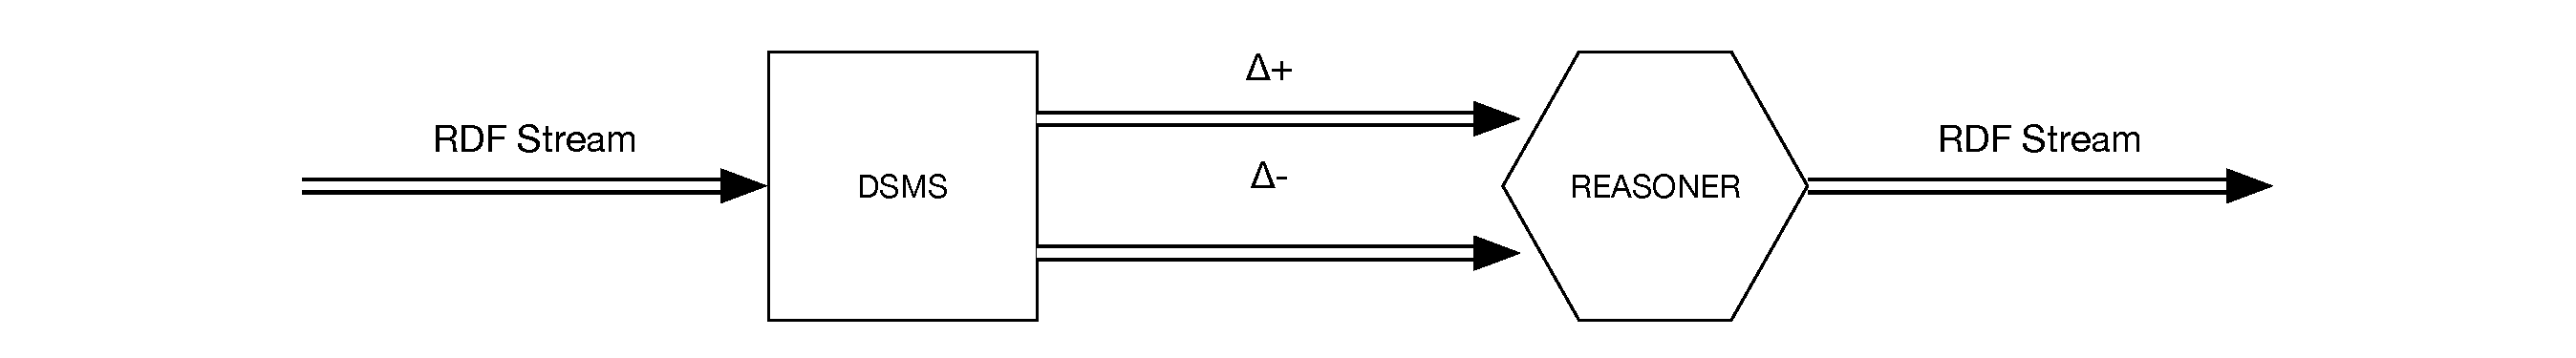
\includegraphics[width=\linewidth]{images/baseline-b}
}
	\caption{The Architecture of \name Baselines: Naive (A) and Incremental (B) Reasoning Approach}
	\label{fig:baselines}
\end{figure}

\noindent RSP Engine are those systems that can apply reasoning techniques upon rapidly changing information encoded in RDF (RDF Stream) and allow to continuous querying on the data stream (Section \ref{sec:rspengine}). It possible to develop RSP Engine following the approach described above, which actually requires to develop the integration of two existing technologies, DSMS and reasoner, and to define how they can communicate. Following we describe how this design model fulfil the requirements we posed in Section \ref{sec:requirements}.

Baselines \textit{Elementarity} can be granted by choosing a DSMS which is a reliable solution in the Information Flow Processing context and the a general purpose rule engine which is comparable with mature solutions. \textit{Elementarity} is reached when the couple elements are simple and valid terms of comparison w.r.t the state of the art.

Baselines \textit{Relevance} requires to cover all the most important theoretical variants that the "pipeline approach" conveys. In terms of reasoning we can choose between two possible approaches and with reference to the data stream processing the choices are again two. Four baseline implementations cover these two main design decisions about the RDF Stream Model and the Reasoning procedures. 

The RDF Stream model describes how the input RDF Stream is processed, different systems accept data in different models, which depends on how RDF Stream is considered in terms of events contemporaneity. The two most relevant ones are:

\begin{itemize}	
\item Triple-based model, where the events pushed in the DSMS are timestamped triples. The timestamps are non decreasing, different triples could have the same timestamp to denote that they are contemporary.
\item RDF Graphs-based: the event pushed in the DSMS are timestamped RDF graph. The timestamps are increasing and the graph is used as a form of punctuation \cite{Tatbul2003b} to separate consequent portions of the RDF stream.
\end{itemize}

The Reasoning Architecture, the techniques to make inference, depends on the way data flow from the DSMS to the reasoner. Two reasoning solutions exist for the two triples data flow:

\begin{itemize}
\item Naive solution: (Figure \ref{fig:baselines}-A) the DSMS produces an RDF Snapshot of the current windows. It sends the entire content of the window to the reasoner, which materialises all the implied triples at each cycle. This is the approach implemented in the C-SPARQL Engine \cite{DBLP:journals/sigmod/BarbieriBCVG10} and in Sparkwave \cite{DBLP:conf/debs/KomazecCF12}.
\item Incremental solution (Figure \ref{fig:baselines}-B) the DSMS outputs the IRStream, the differences between the current window and the previous one. The $\Delta^{+}$ snapshot contains the triples that have just entered in the window, while the $\Delta^{-}$ snapshot contains the triples that have just exited from the window. The reasoner, using $\Delta^{+}$ and $\Delta^{-}$, incrementally maintains the materialisation over time. This approach is taken as term of comparison in \cite{DellAglio2014} and it is inspired from \cite{DBLP:conf/cikm/RenP11}.
\end{itemize}

Baseline \textsc{Eligibility} requires to check out all the performance measurements involved by the RSP Engine in use. We already stated that the choice of the DSMS and the reasoner may affect baseline \textsc{Elementarily}, but they also influence the performance of the engine. In order to be Eligible the Baselines must be comparable with mature solutions in terms of degree of magnitude. As reported in Section \ref{sec:teststand}, we take as initial measure set: Latency, Memory and of the query results Completeness and Soundness. Latency and Memory are the metrics upon which the comparison can be built. Further consideration can be done for Completeness and Soundness w.r.t recent work on correctness \cite{DBLP:conf/semweb/DellAglioCBCV13}  \cite{DBLP:conf/semweb/DellAglioCBCV13} explains the importance of external control on time to assure that the RSP Engine always outputs the correct answers (even when overloaded). The proposed Baselines should take advantage of the ability of some DSMS to be temporally controlled by an external agent by sending time-keeping events to synchronise the internal time flow. In this wat is possibile to ensure Completeness and Soundness even in case of high stress condition for the Baselines. %One time-keeping event is sent before injecting the triples in a \textsc{TCEvent} and another one after all triples in \textsc{TCEvent}  were sent. In this way all the triples in the TCEvent are consider contemporary by the 

Finally, baselines \textsc{Simplicity} comes from those parameters that directly influence the RSP Engine: the query $\mathcal{Q},$ and the entailment regime. $\mathcal{Q}$ should be eligible in terms of reasoning which means having an high materialisation effort of the implicit information entailed by the content of the window, given the ontology chosen by the user. The entailment regime should be a fragment of a language, maybe RDF-S, which reduces complexity but preserves the normative semantics and the core functionalities. Moreover, what we state above about externally time control clarifies the system workflow providing \textsc{Simplicity} too.

\section{Analyser}\label{sec:analyser}

The \textsc{Analyser} consists, from an engineering point of view, in one or more automated procedures that process the experiment results transforming raw data into an human-readable form. Actually, not all the analysing procedures can be completely automated and data analysis can not be always generalised. For this reason we decide to design the \textsc{Analyser} from a research point of view. It can bee seen as set of methods for data processing and analysing, which allow to refute or confirm hypothesis and to improve existing models trough empirical findings.

In this Section we focus on the definition of the methods that compose the analysis, while in Section \ref{sec:analyser-impl} we detail much more which tools sustain the investigation at different levels, allowing data visualisation and deeper statistical investigations.

\begin{figure}[tbh]
  \centering
	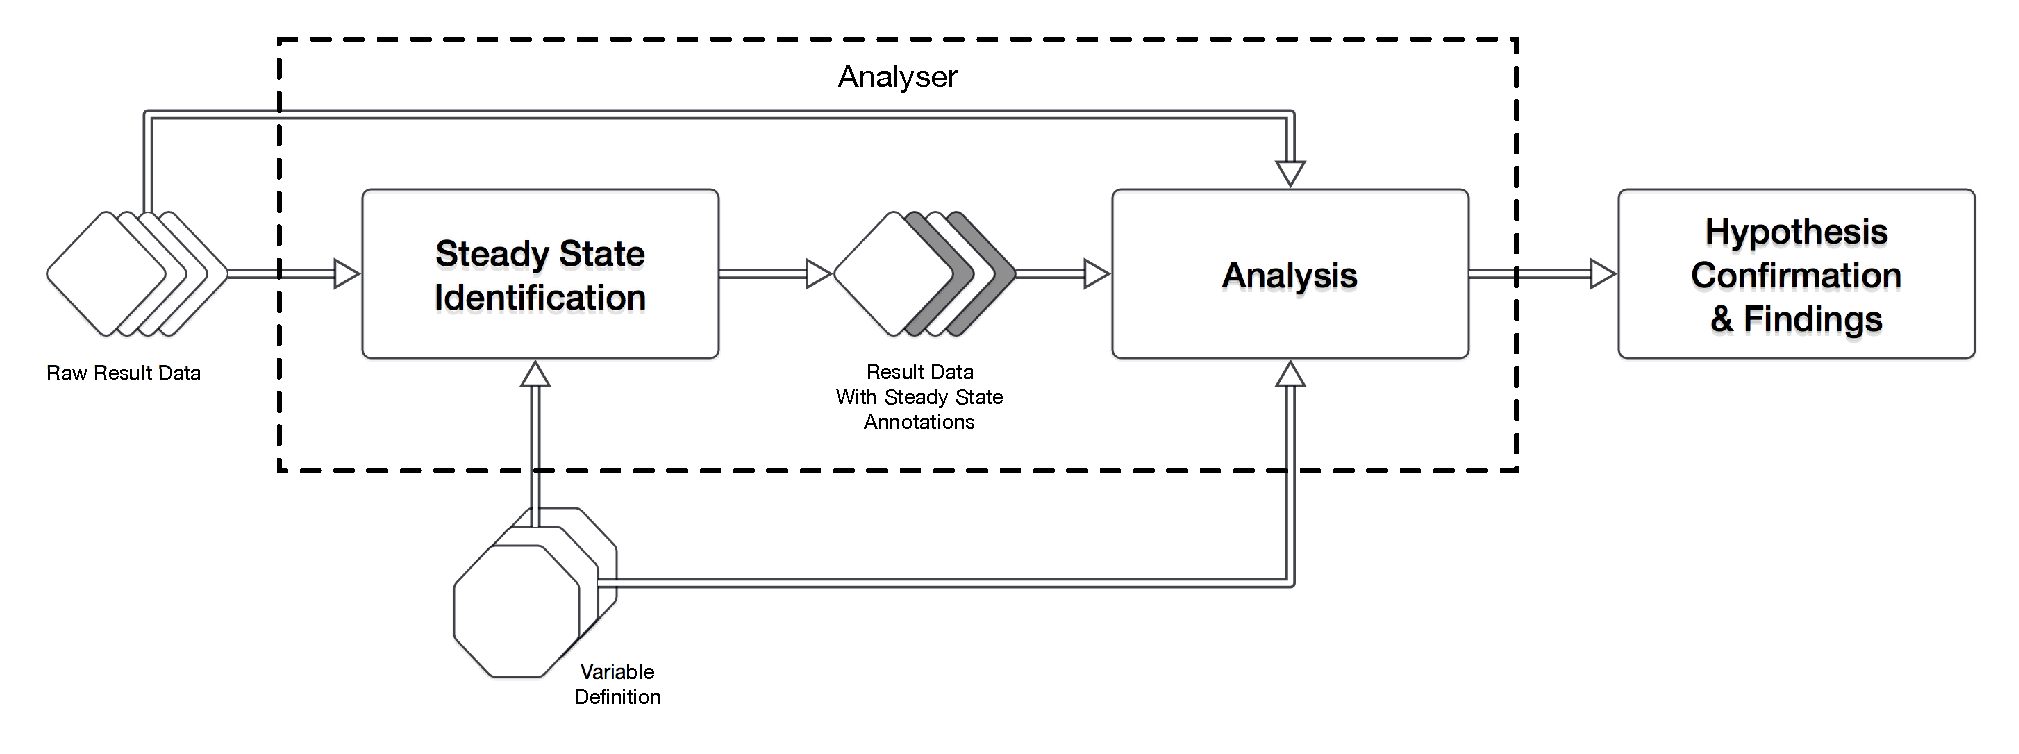
\includegraphics[width=\linewidth]{images/analyser-block-schema}
	\caption{\textsc{Analyser} Block Schema} 
  	\label{fig:analyser-block-schema}
\end{figure}

Figure \ref{fig:analyser-block-schema} shows the different phases of the data processing. The methods that compose the \textsc{Analyser} can be divided into three main block, each one with different supporting tools and different goals.

\textsc{Analyser} takes as input the raw data produced by the \textsc{Test Stand} by executing the experiment, and the variables on which the analysis will be based on. The \textsc{Test Stand} outputs raw data are in times series format and which data it outputs depend on the users needs. The \textsc{Test Stand} measurement set may variate according to the requirement [R.7]. To this extent the \textsc{Analyser} should be extendible too, and the variables of the analysis must be seen as an input provided by \name user.

To properly compare results between $n$ different RSP Engines data must be standardized. In the \textit{Steady State Identification} Block data are processed according to the variables, identifying which variable has reached a Steady State condition.

The last step in the high level Analyser Block Schema consists in the formalisation of theoretical results. The aim of this step is obviously confirm or refute hypothesis formulated at experiment design level. However, \name has the aim of sustaining the empirical research over RSP Engine which allow a new kind of observation that may improve existing theoretical models of the Stream Reasoning area.

In the next subsection we provided further details on the \textit{Steady State Identification} Block, Subsection \ref{sec:analyser-ss-block}, and about the \textit{Analysis} Block, Subsection \ref{sec:analyser-analysis-block}. The Theoretical Result Block it is not described because it depends on \name user and can not be formalised yet.

\subsection{Steady State Identification Block}\label{sec:analyser-ss-block}

\begin{figure}[tbh]
  \centering
	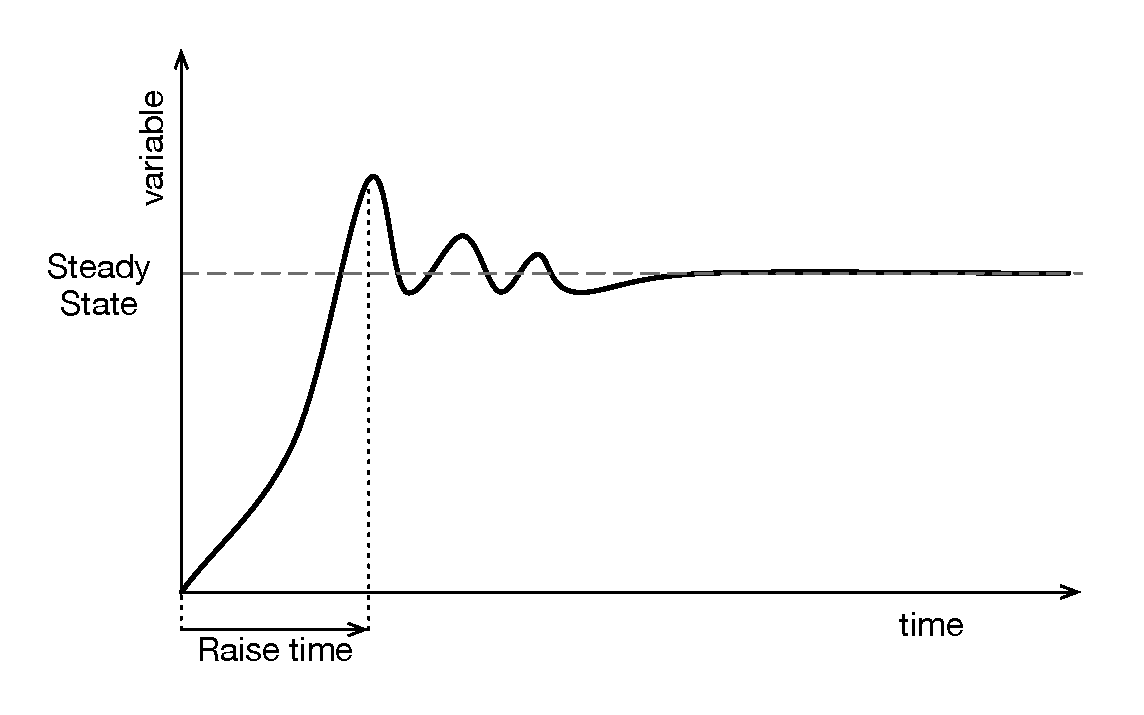
\includegraphics[width=0.5\linewidth]{images/steady-state}
	\caption{Time Series Behaviour Example in Temporal Domain} 	
  	\label{fig:steady-state}
\end{figure}

The \textit{Steady State Identification} (SSI) Block is first element in Figure \ref{fig:analyser-block-schema}. In general it applies a pre-analysis of the raw data. It outputs if a given variable of the tested RSP Engine has not reached the Steady State condition , which is the moment when a dynamic system reaches the equilibrium for a certain variable. The SSI is a common passage in almost any research on dynamic system, because those systems usually have an initial transitory phase which inhibits generalisation and comparisons. Figure \ref{fig:steady-state} shows the typical behaviour in the time domain for a certain variable and also evidences the point when the series reaches the Steady State condition. The \textit{Steady State Identification} Block allows to understand the degree of reliability of the data, how we can assume a certain observation is confirmed and generalizable. % 


\subsection{Analysis Block}\label{sec:analyser-analysis-block}

Once the Steady State is identified, it is possible to proceed with the central data analysis, which is summarised in Figure \ref{fig:analyser-block-schema} by the \textit{Analysis} Block. This Block exploits the \textit{Steady State Identification} output to study the transitory phase, which is a crucial part of the dynamic system comprehension and thus of the Hypothesis confirmation.

The investigation can be decomposed in four levels within the \textit{Analysis} Block, with increasing details degree and different goals.  Figure \ref{fig:analysis-method} is a graphical representation of the investigation stack implemented within the \textit{Analysis} Block, the detail level grows from the top to the bottom.

Before presenting the stack level one by one, we introduce two concepts about the experiment analysis:
\begin{itemize}
\item \textit{Intra Experiment Comparison} -  it means building comparisons between variables upon a single, well-determined experiment $,<\mathcal{E},<\mathcal{D},<\mathcal{T},<\mathcal{Q}>$.
\item \textit{Inter Experiment Comparison} -  it means building comparisons of different experiment 
$,<\mathcal{E},<\mathcal{D},<\mathcal{T},<\mathcal{Q}>$ and $,<\mathcal{E}',<\mathcal{D}',<\mathcal{T}',<\mathcal{Q}'>$ upon a single variable. Usually, the compared experiment differs at most for one or two elements in the tuple. 
\end{itemize}


\subsubsection{Level 0 - Dashboards}\label{sec:heaven-level0}

Dashboards are the highest level of analysis offered by \name for \textit{Inter-Experiment} comparison. Some statistical values like average (or maximum, minimum, median ecc) are presented in a n-dimension radar plot, as the one in Figure \ref{fig:radar}, which involves all the variables selected during the experiment design phase. Visual comparison of the data trough dashboards is natural when few variable are involved. It is easy to compare many solutions and identify which one is the best. The aim of dashboard is to compare experiments and pointing out the relation that occurs among the involved variables.

\begin{figure}[tbh]
  \centering
	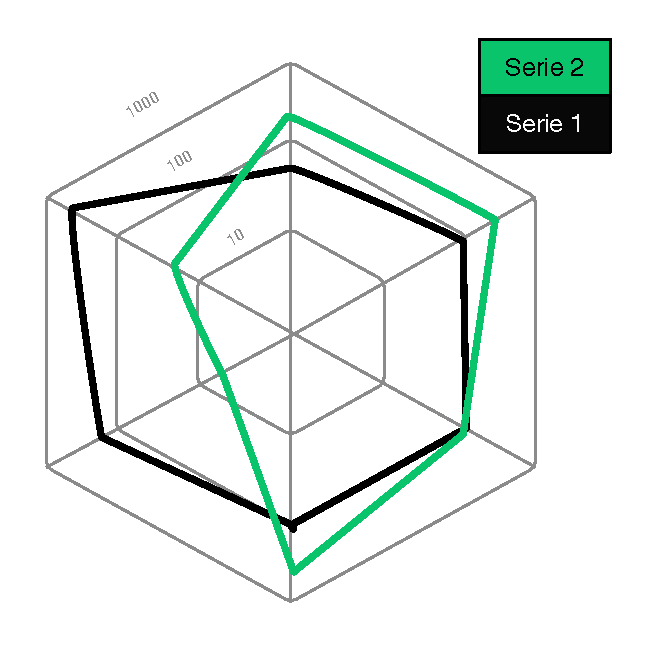
\includegraphics[width=0.5\linewidth]{images/radar-plot}
	\caption{Dashboard Example - Radar Plot} 	
  	\label{fig:radar}
\end{figure}

The idea of a single visualisation method which allows to answer to any hypothesis is desirable, but not probable.  Unfortunately, the reliability of the methods depend on the system complexity and not only on the complexity of the method itself. Thus, this level of analysis may not be able to represent the entire system complexity. The Steady State condition represents another point of weakness. If it is not reached by all the variable involved, the analysis generalisation can not be granted and dashboard relevance becomes frail. Further levels of analysis are required, at least for a better comprehension of those unpredictable results that refute even naive hypothesis, formulated on well known theoretical truths.


\subsubsection{Level 1 -  Statistical Values Comparison}\label{sec:heaven-level1}

This Analysis level focuses on a single variable at time (Latency, Memory ecc.), in a certain statistical condition (Maximum, Minimum, Mean Value ecc.) exploiting \textit{Inter-Experiment} comparison. 

To verify an hypothesis researches design and execute multiple experiments which variates for few parameters. This analysis is focused on the entries experiment set. The experiments must be arranged into an smart layout that highlights the differences between experiments upon one or more well-defined characteristics. The analysis involves one variable at time, comparing the results over the experiment set. 

The aim of Level 1 is identifying which parameter, if any, determines behaviour of the solution w.r.t the observed variable. \name enables two possible analysis approaches within Level 1:
\begin{itemize}
\item \textit{Quantitative} -  The comparison results are present in percentage form, quantifying how much a solution is better than another one under some conditions. 
\item \textit{Qualitative} - it is a simplification of the Quantitative approach. Sometimes we only need to understand which solution is the best, without focusing on numeric values. The Qualitative approach requires the definition of a tolerance threshold, for example 5\%, to distinguish when a solution is better, worse or equal to another one.
\end{itemize}

\subsubsection{Level 2 - Patter Identification}\label{sec:heaven-level2}

The comparison of a single statistical value over multiple variable (Level 0) or a single one (Level 1) may be not sufficient to explicit the RSP Engine behaviour. Starting from Level 2, visual analysis for \textit{Inter-Experiment} comparison is introduced. As in Level 1 the investigation involves a single variable over the entire experiment set, disposed into an easy-to-ready layout which points out experiment differences. Level 2 instead enables the comparison of the experiment set, presenting result data in a graphical way, which shows the system behaviour over all the experiment execution.

The aim of this level is evidencing if a certain variable a some patterns among the experiment set. How to choose the correct graphical representation depends on the variable nature and requires specific analysis. However, the most common ones for time-series are time domain form, value distribution or frequency domain representations. In general Level 2 allows to visualise how the system behaves, which is not visible with a mere model investigation.

\subsubsection{Level 3 - Visual Comparison}\label{sec:heaven-level3}

The Level 3 is the bottom level of the investigation stack. It focuses on a single solution at time and it exploits both \textit{Inter-Experiment} comparison, with the aim to understand how different experiment execution are related or to  \textit{Intra-Experiment} comparison, with the goal of pointing out the relation between the variables over all the experiment. In the first case, Level 3 reproduces the Dashboard idea but over all the experiment execution. In the second case instead, it extends what done in Level 1 and 2, but focusing on a single visualisation at time.

\begin{figure}[htb]
  \centering
	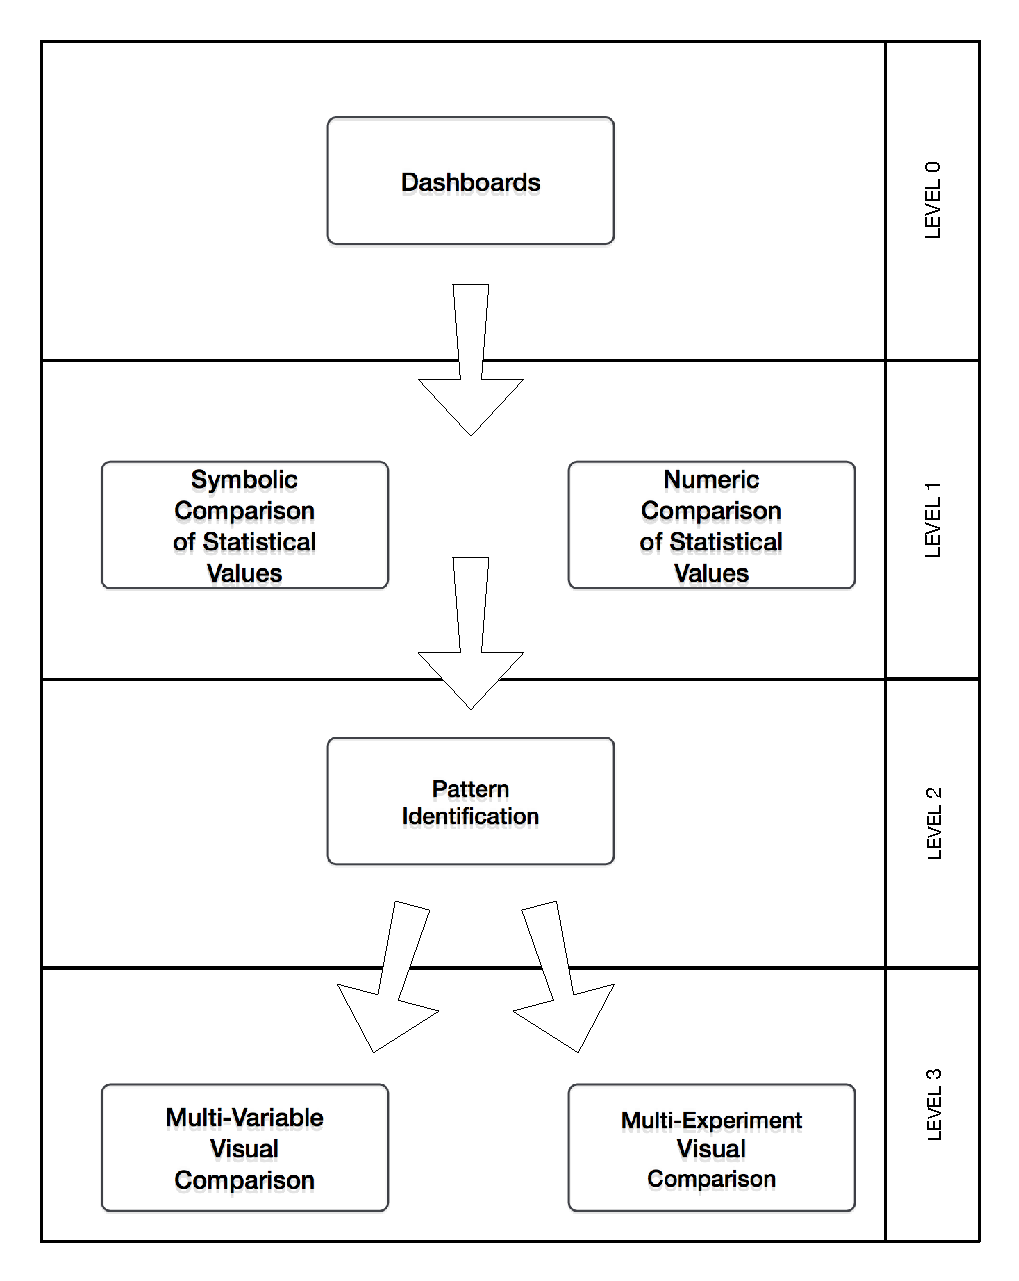
\includegraphics[width=\linewidth]{images/analysis-method}
	\caption{\textsc{Analyser} Investigation Stack}
  	\label{fig:analysis-method}
\end{figure}



 \clearemptydoublepage
%\section{Heaven}\label{sec:impl-intro}

In Chapter \ref{chap:problem-settings} we posed the requirements that any solution must fulfil, in order to properly answer our research question. Then in Chapter \ref{chap:heaven} we face each requirement at design level, stating how one possible implementation of \name must be realised to fulfil them. 

In this chapter we describe our implementation experience of \namens: 
Firstly in Section \ref{sec:abstractions} we present the pillars concepts of this development. In Section \ref{sec:data-impl} we describe the data model of the \textsc{Test Stand} and the \textsc{Analyser}. In Section \ref{sec:modules-impl} we introduce each \name module: the \textsc{Streamer}, the \textsc{ResultCollector} and the \textsc{Test Stand Supporting Structure}. In Section \ref{sec:baselines-impl} we describe how we implement four baseline RSP Engines and finally, in Section \ref{sec:analyser-impl}, we describe how the \textsc{Analyser} Implementation Stack is realised w.r.t the Evaluation we will present in Chapter \ref{chap:evaluation}.

\section{Event Processor}\label{sec:abstractions}

The architecture of the \textsc{Test Stand} consists in three stand alone modules that establish a mono-directional communication flow: \textsc{Streamer}, \textsc{RSP Engine} and \textsc{Result Collector}. 

\begin{figure}[h!tb]
  \centering
	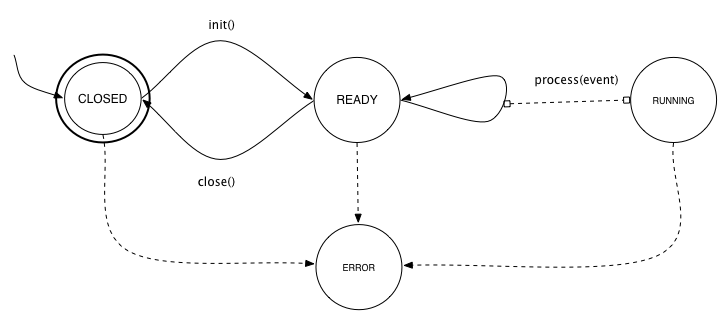
\includegraphics[width=\linewidth]{images/fsm-schema}
	\caption[\textit{EventProcessor} States Diagram]{The finite state machine diagram of any \name module and the Baselines. It is realised trough the \textit{Startable} interfaces, which provide the \textit{init()} and \textit{close() }methods, and trough the \textit{EventProcessor} interface, which declares the \textit{process(Event e)} method. The execution is possible only during the RUNNING state, which can be achieved by one and only module at time, as a constrain. The ERROR state prevents the propagation of erroneous behaviour to the data.}
  	\label{fig:module-fsm}
\end{figure}

Among all the requirements reported in Section \ref{sec:requirements} two of them are immediately relevant: [R.10], i.e. the need of an \textit{Extendible Design}, and [R.11], which states the necessity of an \textit{Event-base architecture} to properly face any RSPEngine. In order to to fulfil both \textsc{Test Stand} requires two main abstractions:
\begin{itemize}
\item The \textit{Event} - which is required to build a hierarchical communication. Indeed, the \textsc{Test Stand} may handle three events flows: one internal to the RSP Engine module, one for the communication between modules and one to communicate with the user. Next section about data clarifies the communication structured. 
\item The \textit{Event Processor} -  which guarantees the system to be modular, it standardizes the interaction simplifying the behaviour of each component in the system. Thus, a module is an \textit{Event Processor} which can be positioned everywhere in the the \textsc{Test Stand} pipeline
\end{itemize}

\pagebreak

\noindent The requirement [R.4] directly influences the workflow of the \textsc{Test Stand}, quoting from Section \ref{sec:requirements} \textit{The Test Stand must not be running when the RSP Engine is under execution}. 

To cover this requirement we designed the status of each module as a Finite State Machine (FSM), which can work only in those states that allow processing (READY). 

The schema in Figure \ref{fig:module-fsm} represents the FSM that each module of \namens, the Baselines, and also for the \textsc{Test Stand External Structure} implements. 

The \textit{Startable} Interface standardises two methods, \textit{init()} and \textit{close()} which allow to control the behaviour of the module at the beginning and the end of the execution. The interface allows to move from the CLOSED state to the READY trough the \textit{init()} method and from the READY to the CLOSED trough the \textit{close()} method. 

The diagram is completed by the \textit{process (Event e)} method, which belongs to the \textit{EventProcessor} interface, The method brings the module into the RUNNING state until the processing ends, and then back to the READY one. As a constrain, one and only one module can be in the RUNNING state in a certain moment during the execution.

Finally, ERROR State, which can be reached from any point of the execution, prevents the propagation of errors over result data: when a module fails the execution is stopped without saving the erroneous data (last event) and reporting the error to the user.

Thus, each \name module implements the \textit{EventProcessor} and the \textit{Startable} interfaces in order to provide the behaviour presented in Figure \ref{fig:module-fsm} by the FSM, fulfilling [R.10] and [R.11]. Moreover,  [R.4] is fulfilled since each module in the systems allows to be to explicitly controlled by the \textsc{Test Stand Supporting Structure}, which starts and stop the processing according to the RSP Engine execution status (see Section \ref{sec:teststand}). 

\pagebreak

\section{Events and Data}\label{sec:data-impl}

We already stated in the previous section that the \textsc{Test Stand} and its modules exploit an Event-based communication, as required by [R.11]. Chapter \ref{chap:heaven} describes \name workflow and how it exchanges events during the execution. Each event represent different data, depending on it position in the workflow. The \textit{Event} concept we introduced, which is implemented as an interface, allows to build the communication in many levels. In general \name handles four kinds of event, which are reported in Figure \ref{fig:uml_events} and defined as follow:

\begin{figure}[h!tb]
  \centering
	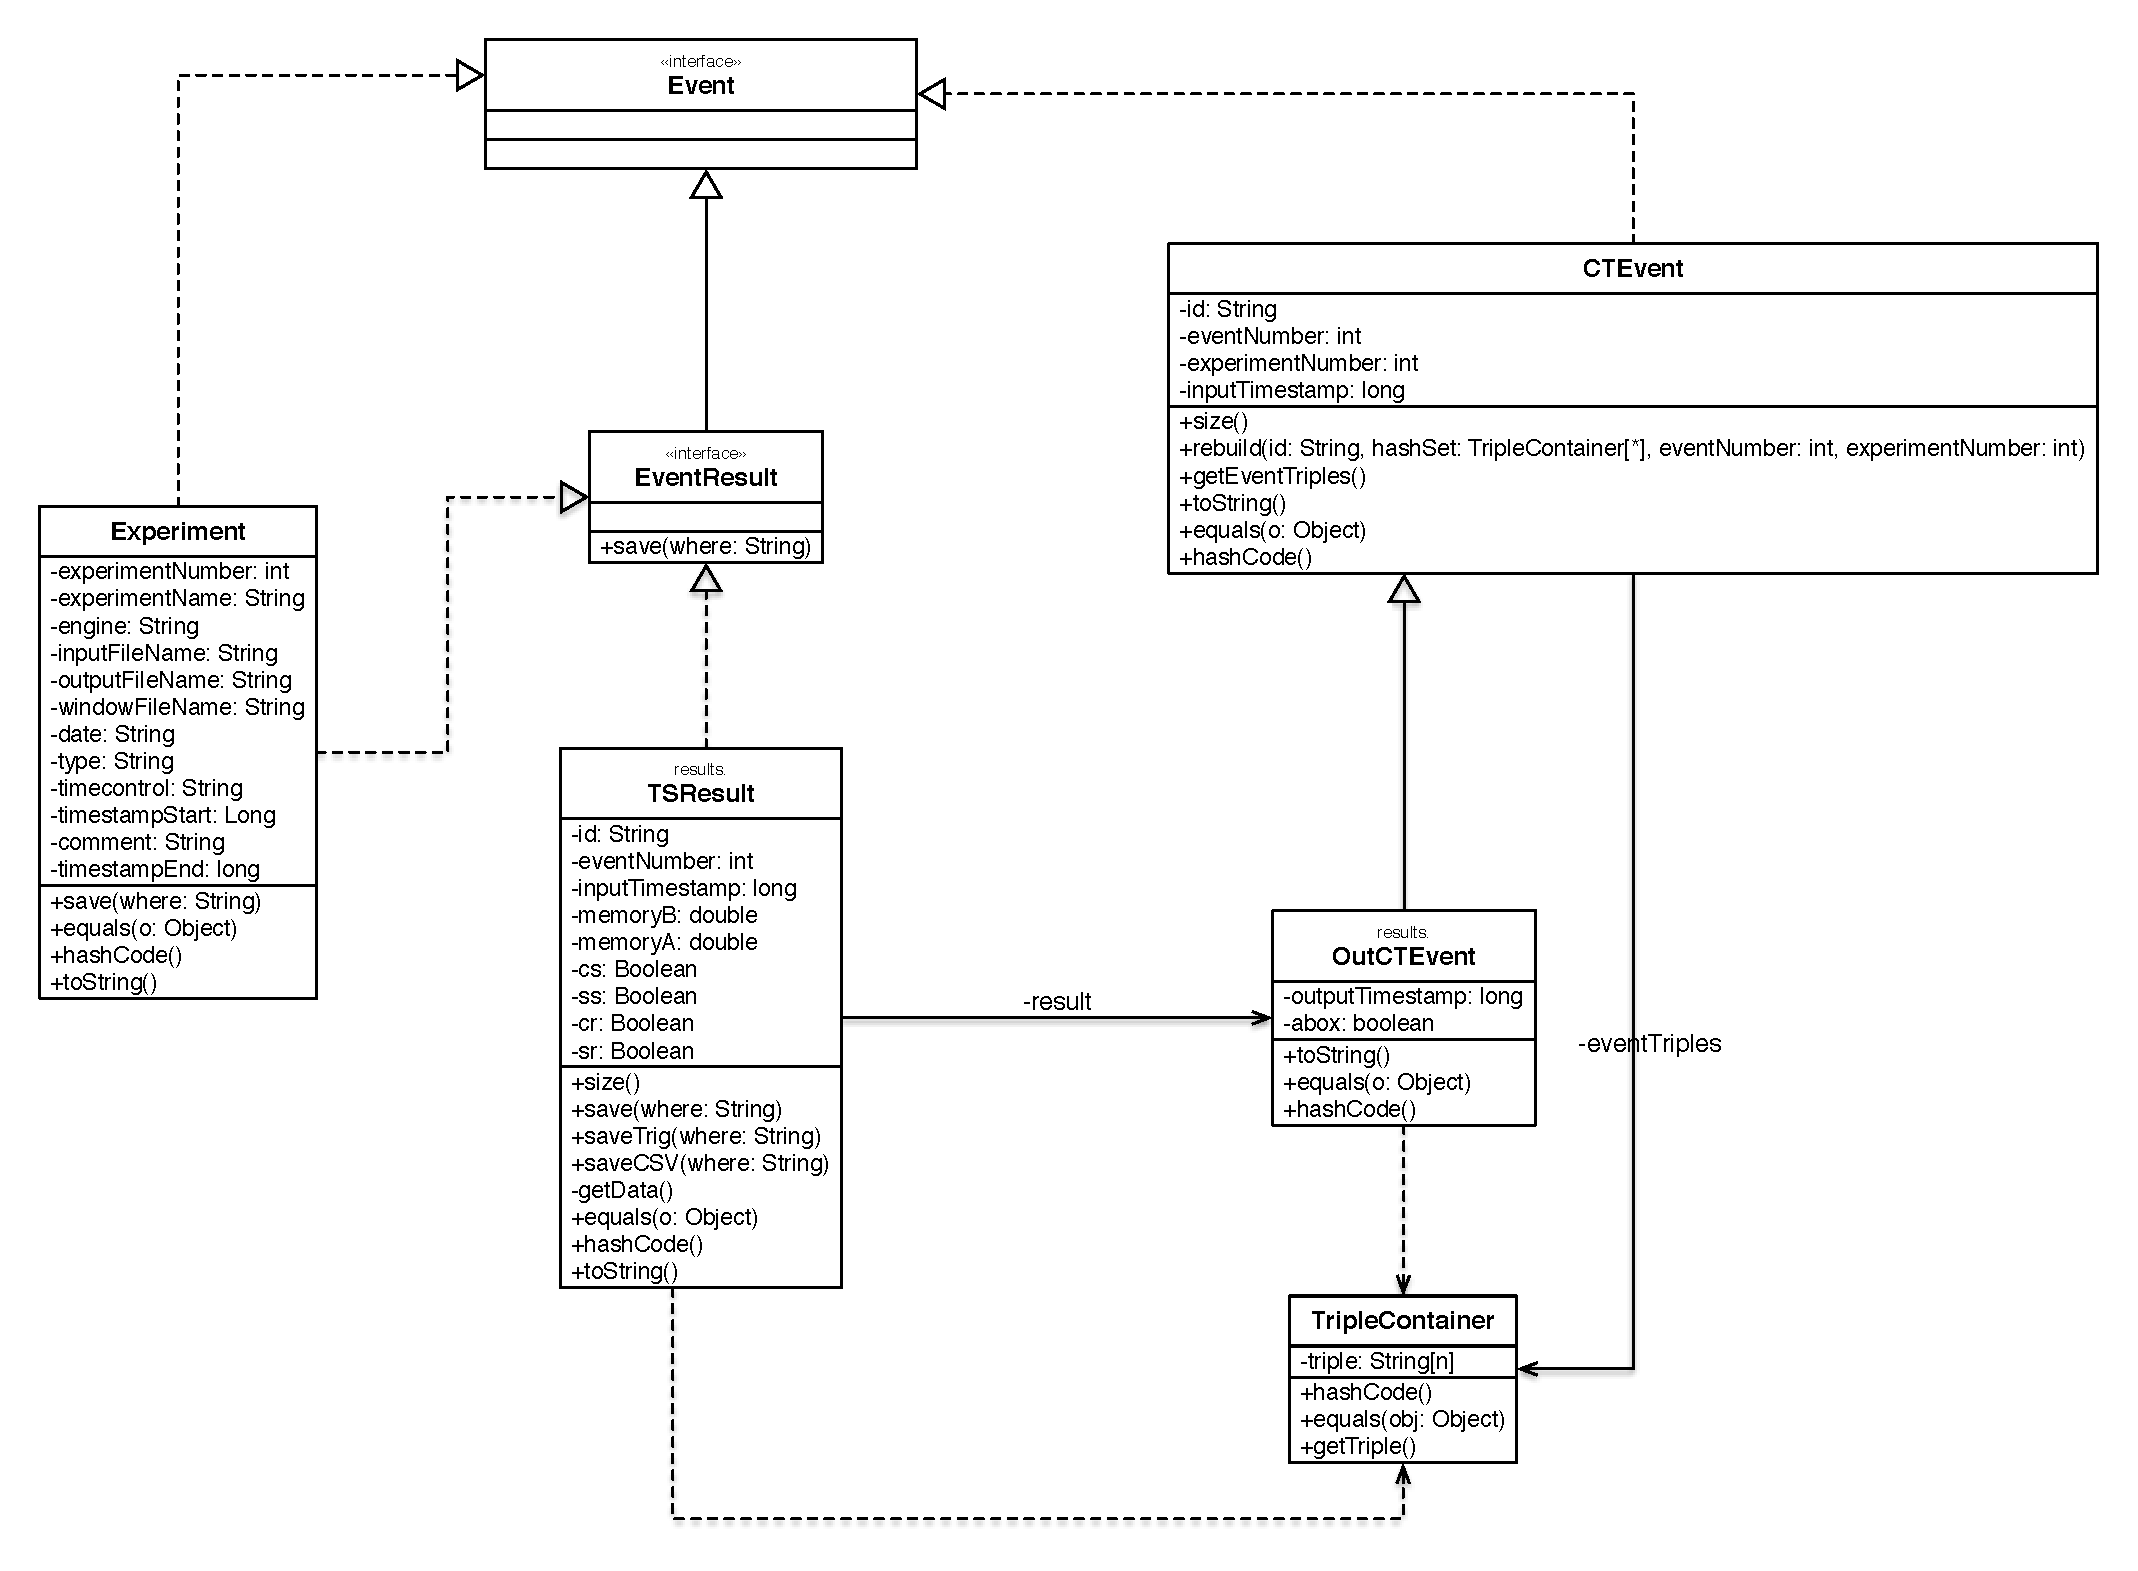
\includegraphics[width=\linewidth]{images/uml_events}
	\caption[\name Execution Events - UML Schema]{The figure shows the event that \name \textsc{Test Stand} and its modules 	exchanges during the execution of an experiment. All of them implement the \textit{Event} interfaces that start the class 	hierarchy.} 
	\label{fig:uml_events}
\end{figure}

\begin{itemize}
\item \textit{Experiment} - it represents the tuple $<\mathcal{E}, \mathcal{D},\mathcal{T},\mathcal{Q}>$, indicating which RSP Engine will be tested and with which queries, data and ontology will be used. It indicates if the current implementation of the engine exploit external timing. Finally the $type$ parameter indicates which kind of testing will be applied (SOAK o Stress for example) and it contains also the execution start time or end time.
\item \textit{CTEvent} - it contains a set of contemporary triples, wrapped in the \textit{TripleContainer}, which allows us to redefined hashcode and equals as a relation of the subject, object and predicate of the RDF triple. The id identifies the event within the experiment.
\item \textit{OutCTEvent} - it represents the event produced by the RSPEngine after processing the active window. Figure \ref{fig:uml_events} show the inheritance relation between \textit{CTEvent}:  \textit{OutCTEvent} extends the \textit{CTEvent} adding the outputTimestamp field.
\item \textit{TSResult} - it wraps the \textit{OutCTEvent} adding the information about the minimal sensor data: memory, sampled ante e post processing, and latency. Two boolean fields allow complete and soundness result, if it is evaluated at runtime (see Section \ref{sec:requirements})
\end{itemize}

\name requires an initialization phase to prepare and input the \textit{Experiment} into the \textsc{Test Stand}. The current implementation exploits a property file with the Experiment parameters: ID and the tuple $<\mathcal{E}, \mathcal{D},\mathcal{T},\mathcal{Q}>$. 

The \textit{CTEvent} and the \textit{OutCTEvent} contain RDF triples in NT-Triple\footnote{http://www.w3.org/2001/sw/RDFCore/ntriples/}, which is the easiest RDF serialisation to parse. This serialisation was chosen to fulfil requirement [R.12], which demands an \textit{Easy-to-Parse RDF Serialisation for the events presented to the RSP Engine in exam}. Figure \ref{fig:uml_events} shows also that the RDF Triples are stored in the events into the \textit{TripleContainer} wrapper: we redefine the triple hashcode and equals method guaranteeing their uniqueness of within an \textit{CTEvent} or \textit{OutCTEvent}.

\section{Modules}\label{sec:modules-impl}

In this section we present the three modules which compose \namens, the \textsc{Streamer} and the \textsc{ResultCollector}, and also the \textsc{Test Stand Supporting Structure}. They all extend the \textit{EventProcessor} and the \textit{Startable} interfaces as reported in Section \ref{sec:abstractions}.

In Section \ref{sec:impl-intro} we define a module a an \textit{Event Processor} which can be positioned everywhere in the the \textsc{Test Stand} pipeline. We state that a module must implements the \textit{Startable} interface, which completes the FSM schema in Figure \ref{fig:module-fsm} with the \textit{init()} and \textit{close()} methods.
Thus, each modules in this section offers three standard methods to interact with them: \textit{process(Event e)} from \textit{EventProcessor} and \textit{init()} and \textit{close()} from the \textit{Startable} Interface.

\subsection{Streamer}	\label{sec:streamer-impl}
\begin{figure}[tbh]
  \centering
	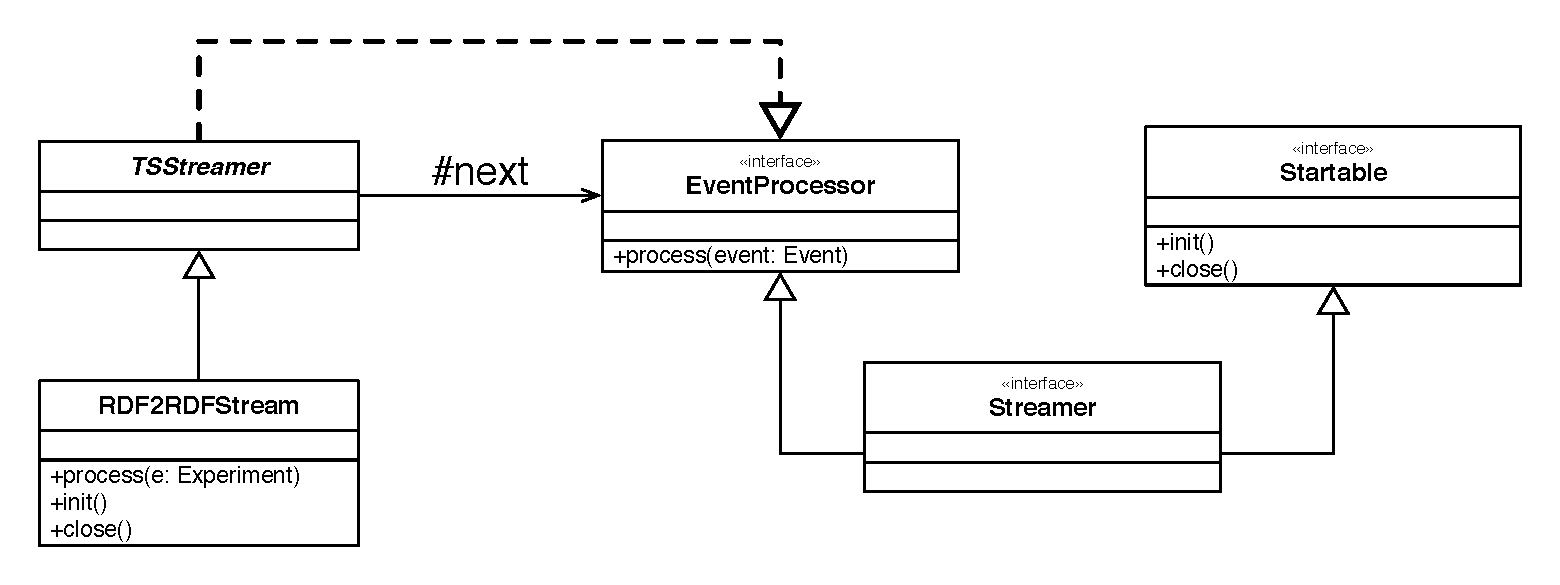
\includegraphics[width=\linewidth]{images/uml_tstreamer}
	\caption[\textit{RDF2RDFStream \textsc{Streamer} Implementation} - UML Schema]{Current implementation of the \textsc{Streamer} module. \textit{RDF2RDFStream} extends the \textit{TSStreamer} abstract class, which defines the module as an \textit{EventProcessor} of \textit{Experiment}s} 
  	\label{fig:uml_tstreamer}
\end{figure}

\noindent Figure \ref{fig:uml_tstreamer} shows the current implementation of the \textit{Streamer} interface, which starts the \textsc{Test Stand} pipeline. Actually, the \textit{Streamer} is implemented as the \textit{TSStreamer} abstract class, which is specialised into processing of \textit{Experiment} events. 

The \textit{Experiment} events are  externally instantiated and then \textit{TSStreamer} receives them, and if initialised it can start the processining. It communicates with another \textit{EventProcessor}, called \textit{next} which can receive  \textit{CTEvent}s and it is represented in Figure \ref{fig:uml_tstreamer} by the labelled arrow.  Notice that also the \textit{next} must be initialised before starting the communication, otherwise the ERROR state will be reached when the event is received by the \textit{next}, because the processing is not allowed.

Figure \ref{fig:uml_tstreamer} contains also the \textit{RDF2RDFStream} implementation, whose internal structure can be seen in Figure \ref{fig:uml_flowrateprofiler}. The \textit{RDF2RDFStream} was developed to conduct experiments as they are presented in Chapter \ref{chap:evaluation}.  It is worth to note that we use LUBM Benchmarks to generate the data for the experiments. LUBM generated data are static, thus the \textit{RDF2RDFStream} builds an RDFStream attaching a timestamp to the static data produced by LUBM. %The file is generated using  LUBM(1000,0), which means 1000 different universities with the random generation seed 0. 

\begin{figure}[tbh]
  \centering
	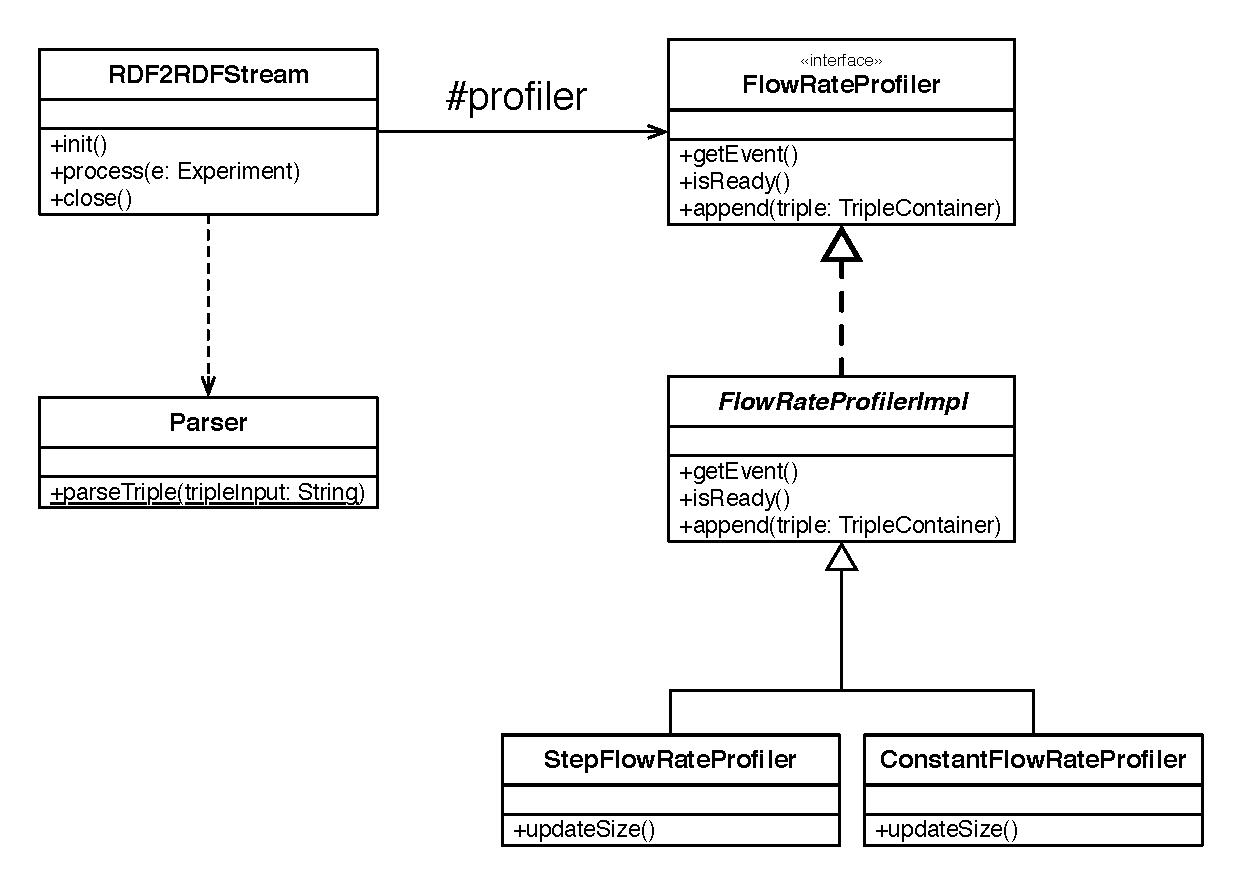
\includegraphics[width=0.75\linewidth]{images/uml_flowrateprofiler}
	\caption[Internal Components of \textit{RDF2RDFStream} - UML Schema]{The \textit{RDF2RDFStream} exploits two subcomponents to build an RDF Stream: the \textit{Parser}, which allows to ready in memory RDF Triples, and the \textit{FlowRateProfiler}, which attaches to RDF triple a timestamp and it builds \textit{CTEvent}s according to a function $f=f(x)$. The \textit{FlowRateProfileImpl} provides implementation of the \textit{append(TripleContainer tc}) method and of the two utility methods \textit{isReady()} and \textit{getEvent()}. Specific implementations of the \textit{FlowRateProfiler} control the function $f$ trough the \textit{updateSize()} method.} 
  	\label{fig:uml_flowrateprofiler}
\end{figure}


The \textit{Parser} component, in Figure \ref{fig:uml_flowrateprofiler} can be accessed statically. It reads in memory one by one the triples in the file guaranteeing data independence [R.1] and it does not influence the memory footprint [R.5] by allocating only the memory necessary to parse a triple. 

Figure \ref{fig:uml_flowrateprofiler} also includes the \textit{FlowRateProfiler}. This component determines the number of triples to add to a \textit{CTEvent} and it builds such an event. In this way, \textit{RDF2RDFStream} can generate different RDF streams to use as $\mathcal{D}$, which differ on the number of contemporary triples in the stream. 

\begin{figure}[tbh]
\centering
\subfigure[Exponential Growing \textsc{CTEvent} Size: $y=2^x$]{
\begin{tikzpicture}
  \begin{axis}[ 
  width=0.4\linewidth,
      height=0.4\textwidth,
    xlabel=$CTEvent$,
    ylabel={$CTEvent Size$},
    xmin=0.00, xmax=40,
	ymin=0, ymax=1048576
  ] 
    \addplot [
    line width=0.75pt]
    coordinates {
    		(0.00, 1.00)
		(1.00, 2.00)
		(2.00, 4.00)
		(3.00, 8.00)
		(4.00, 16.00)
		(5.00, 32.00)
		(6.00, 64.00)
		(7.00, 128.00)
		(8.00, 256.00)
		(9.00, 512.00)
		(10.00, 1024.00)
		(11.00, 2048.00)
		(12.00, 4096.00)
		(13.00, 8192.00)
		(14.00, 16384.00)
		(15.00, 32768.00)
		(16.00, 65536.00)
		(17.00, 131072.00)
		(18.00, 262144.00)
		(19.00, 524288.00)
		(20.00, 1048576.00)
		};	
		
	\end{axis}
\normalsize

\end{tikzpicture}
}
\subfigure[Step Growing Size with K1=100 and K2=1000 after 9 \textsc{CTEvents}]{
\begin{tikzpicture}
  \begin{axis}[ 
  width=0.4\linewidth,
      height=0.4\textwidth,
    xlabel=$CTEvent$,
    ylabel={$CTEvent Size$},
    xmin=0.00, xmax=20,
	ymin=0, ymax=1200
  ] 
    \addplot [
    line width=0.75pt]
    coordinates {
    		(0.00, 100.00)
		(1.00, 100.00)
		(2.00, 100.00)
		(3.00, 100.00)
		(4.00, 100.00)
		(5.00, 100.00)
		(6.00, 100.00)
		(7.00, 100.00)
		(8.00, 100.00)
		(9.00, 100.00)
		(9.00, 1000.00)
		(10.00, 1000.00)
		(11.00, 1000.00)
		(12.00, 1000.00)
		(13.00, 1000.00)
		(14.00, 1000.00)
		(15.00, 1000.00)
		(16.00, 1000.00)
		(17.00, 1000.00)
		(18.00, 1000.00)
		(19.00, 1000.00)
		(20.00, 1000.00)
		};	
		
	\end{axis}
\normalsize

\end{tikzpicture}
}
\caption[Example of FlowRateProfiler Triple Distribution]{The \textsc{FlowRateProfiler} is able to calculate \textsc{CTEvent} size according to a function which relates the number of triple to the number of \textsc{CTEvent} }
\label{fig:frp-examples}
\end{figure}


The \textit{FlowRateProfilerImpl} implements \textit{FlowRateProfiler} interface. It provides a common implementation for the method \textit{append(TripleContainer tc)}, which adds to the current \textit{CTEvent} an RDF triple,  and of the two utility methods \textit{isReady()} and \textit{getEvent()}. What variates between different implementations of this component, is the \textit{updateSize()} method. 

The \textit{FlowRateProfiler} creates \textit{CTEvent} according to a function $y=f(x)$, in which $x$ is the number of the \textit{CTEvent} and it results that $y$ is the number of triple this \textit{CTEvent} will contain. The update logic given by $f$ is implemented within the \textit{updateSize()} method. For example if we decide to increase linearly the number of triples inside a \textit{CTEvent} the function $f$ will be: \[y=x, \text{ where } x,y \in N\]
The first event (E0) will contain zero triple, E1 will contain only one triple following E4 will contain four triples and so forth. Another possibility is to increase exponentially the number of triples inside a \textit{CTEvent} : \[y=2^x, \text{ where } x,y \in N\]The first event (E0) will contain one triple, E1 will contain two triple following E3 will contain eight triples and so forth, Figure \ref{fig:frp-examples}.a shows the resulting behaviour plotting the triple number on y-axis and \textit{CTEvent} number on x-axis.



In the current stage of development we include four implementations of the \textit{FlowRateProfiler}, two of them are related to our experiments: 
\begin{itemize}
\item \textit{ConstantFlowRateProfiler} - it maintains the same number of triples for each events over all the experiment: \\
\[y=K, \text{ where } K \in N \]

\item \textit{StepFlowRateProfiler} - it maintains a constant number of triple $K1$ inside a \textit{CTEvents} for $x$ occurrences, then it suddenly changes the number of triple $y$ form $K1$ to $K2$ where $K2 >> K1$. The number of  \textit{CTEvents} $x$ is specified in the set-up phase of the component.  Figure \ref{fig:frp-examples}.b contains the resulting plot of implemented function which follows:

\[
y=
\begin{cases}
K1, &\text{if $x < M$ } $ where $ K1, M \in N\\
K2, &\text{if $x >= M$} $ where $ K2 >> K1, K2 \in N
\end{cases}
\]


\end{itemize}

The remaining two  \textit{FlowRateProfiler} implementations in \name that are not related to our evaluation are:
\begin{itemize}
\item \textit{LinearStepFlowRateProfile} - it streams $x$ \textsc{CTEvents} of dimension $y$, in terms of triples, then linearly increase the number of a quantity $M$: \[y=x*M, \text{ where } x,y,M \in N\]
\item \textit{ConstantRandomFlowRateProfiler} - it changes $y$ and $x$ according with two random integer generators directed by two seeds. The generators provided integer numbers according to a certain probability \[y=randomInt(seed), \text{ where } random(seed),y \in N\]
\end{itemize}


\subsection{Result Collector} 

\noindent The \textsc{ResultCollector} is the data acquisition system that receives and persist the query results and the measurements data gathered by the \textsc{Test Stand} during the execution of an experiment.

\begin{figure}[tbh]
  \centering
	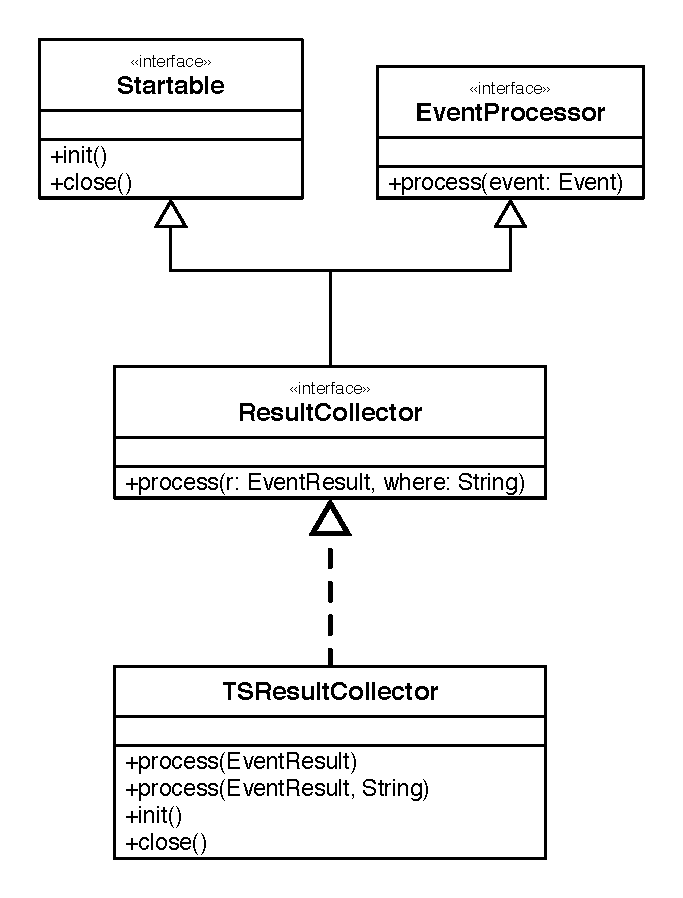
\includegraphics[width=0.5\linewidth]{images/uml_resultcollector}
	\caption[\textsc{ResultCollector} Current Implementation - UML Schema]{The current implementation of the \textsc{ResultCollector} interface is the \textit{TSResultCollector} which processes events that implements the \textit{EventResult Interface}. \textit{ResultEvent} interface hides the saving procedure, delegating the implementation to the event provider trough    the \textit{save()} method. \textit{TSResultCollector} exposes also the method process(Event e, String where), which allows the caller to specify the destination. } 
  	\label{fig:uml_resultcollector}
\end{figure}

The UML Schema in Figure \ref{fig:uml_resultcollector} shows firstly that the \textit{ResultCollector} interface is again an extension of the \textit{EventProcessor} and the \textit{Startable} ones. The current implementation is the \textit{TSResultCollector}, which stays at the end position in the \textsc{Test Stand} pipeline. The \textit{ResultCollector} is responsible of saving data in a way that is independent from which data format, since requirement [R.7] demands to \textit{enable users extensions with new software sensors and specific measurements collection}. The \textit{TSResultCollector} applies a general saving procedure exploiting the \textit{EventResult} interface, which exposes the \textit{save(String where)} method to delegate the implementation of such a procedure to the provider of the event. Figure \ref{fig:uml_resultcollector} shows the relation between the \textit{EventResult} interface and the \textit{TSResultCollector}, which specialises the processing method to \textit{process(EventResult} and it known the general destination of the data, but it also exposes a secondary one \textit{process(EventResult, String where)}, which allows the caller to specify the saving path.


\begin{figure}[tbh]
  \centering
	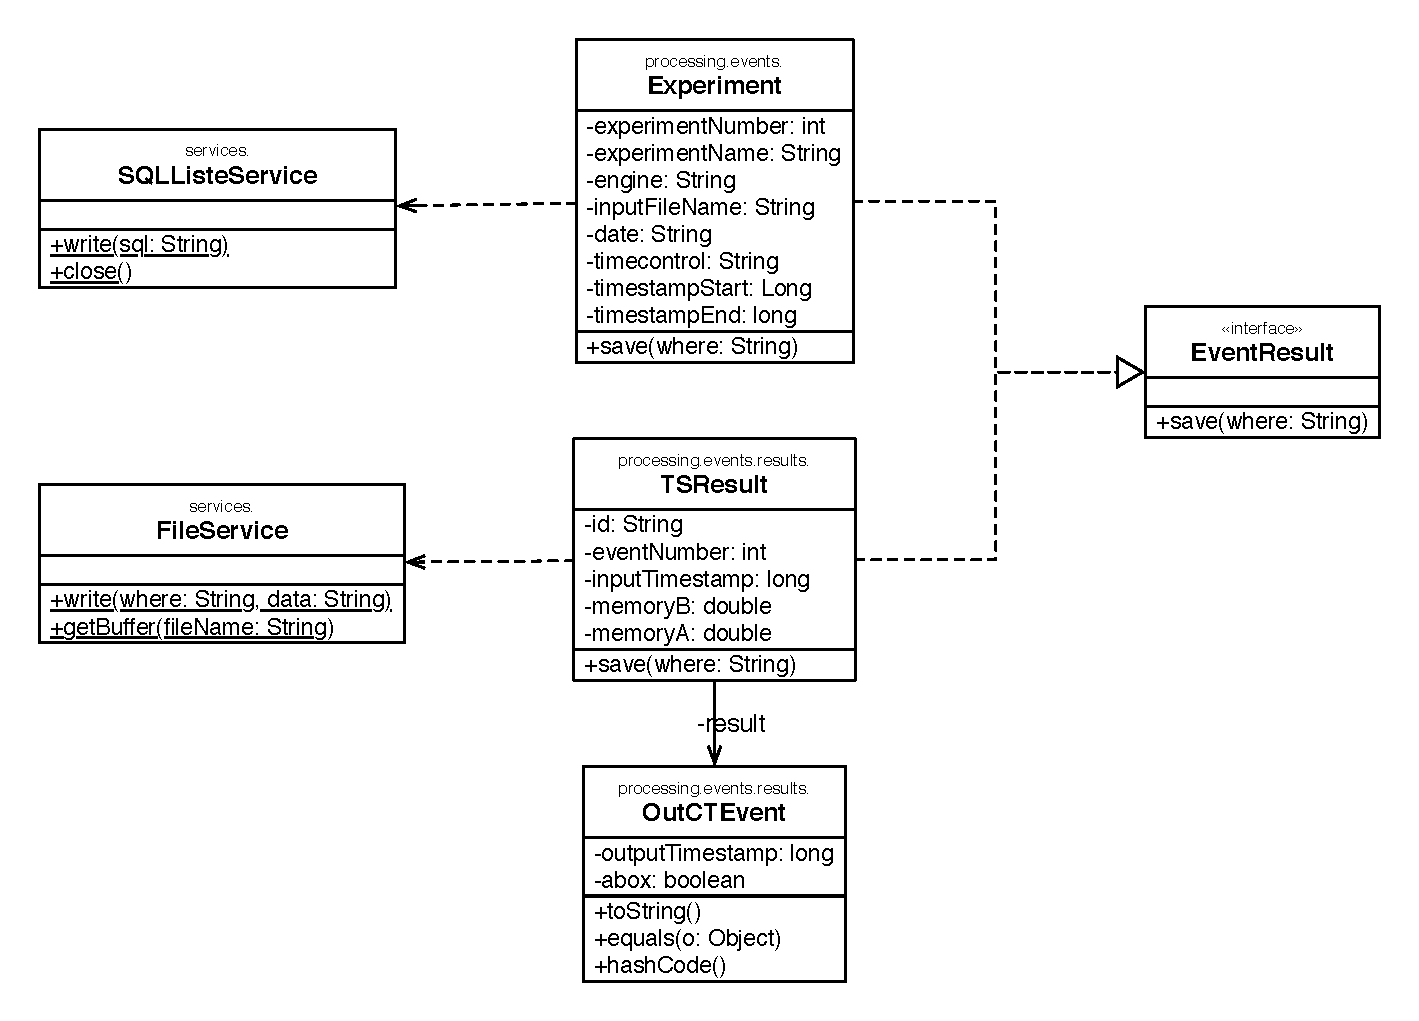
\includegraphics[width=\linewidth]{images/uml_resultcollector_events}
	\caption[\textsc{ResultCollector} Events - UML Schema]{ All the \textit{Experiment}, the \textit{TSResult} and the \textit{OutCTEvent} implements the \textit{EventResult} interface in order to hides specific saving procedure behind the \textit{save(String where)} method. The saving procedures exploits two service classes the \textit{FileService} and the \textit{SQLLIsteService}, which avoid concurrent access to the saving procedure with static methods.} 
  	\label{fig:uml_resultcollector_events}
\end{figure}

Figure \ref{fig:uml_resultcollector_events}, shows how different events in the system exploit the \textit{EventResult} interface. In the current implementation the \textit{TSResultCollector} handles two kinds of event:
\begin{itemize}
\item \textit{TSResult} - it saves the data of the query results into a TriG\footnote{http://www.w3.org/TR/trig/} file where the graph name is the event id inside the experiment, while it saves the measurements data into a CSV\footnote{$http://en.wikipedia.org/wiki/Comma-separated_values$} file that represent the time series w.r.t events id. 
\item \textit{Experiment} - it saves the experiment metadata and the tuple \\ $<\mathcal{E},\mathcal{D},\mathcal{T},\mathcal{Q}>$ collapsed into a generic description field into SQLite\footnote{https://sqlite.org/} database.
\end{itemize} 

Both the saving procedure exploit a service class, respectively the \textit{FileService} and the \textit{SQLLIsteService}. In Figure \ref{fig:uml_resultcollector_events} are describe those services, which expose static methods to interact with the file-system. The goal is reducing system complexity offering a single point of interaction with the file-system. In this way is possible  to avoid parallel interactions that may influence the experiment. 


\subsection{Test Stand Supporting Structure}\label{sec:teststand-impl}


\begin{figure}[tbh]
  \centering
	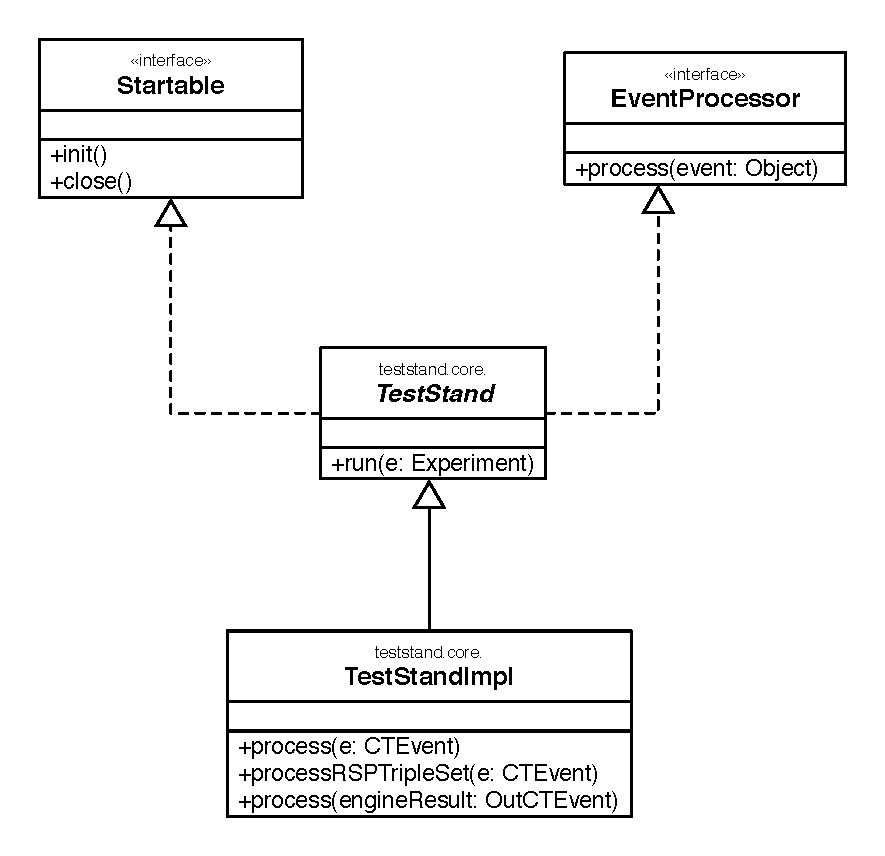
\includegraphics[width=0.5\linewidth]{images/uml_teststand}
	\caption[\name \textsc{TestStand} - UML Schema]{The \textsc{TestStand} abstract class implements both the \textit{EventProcessor} and the \textit{Startable} interfaces, but defines only the methods \textit{init()} and \textit{close()}  and it adds the \textit{run(Experiment e)} method, which encapsulate the execution logic. The \textit{process(CTEvent e)} method is implemented by \textit{TestStandImpl} which represents the \textit{Test Stand External Structure}. It orchestrates the communication between other modules and gather the data.}
  	\label{fig:uml_teststand}
\end{figure}


\noindent \name \textsc{Test Stand} was defined as set of modules which interact exchanging events during the execution. However, Chapter \ref{chap:heaven} describes at the design level the presence of an external structure which orchestrates the communication between the \textsc{Streamer}, the \textsc{RSP Engine} and the \textsc{ResultCollector}. This external structure also exposes the APIs for users interaction. Figure \ref{fig:uml_teststand} represent this idea into an UML schema where the abstract class \textit{TestStand} implements both the \textit{Startable} interface  defining the \textit{init()} and \textit{close()} methods and also the \textit{EventProcessor} interface, but it leaves the implementation of the \textit{process(CTEvent e)} method to the current implementation: the \textit{TestStandImpl}. 

The relation between the \textit{TestStand} and other modules is presented in Figure \ref{fig:uml_teststand_modules}. The \textit{TSStreamer}, the \textit{RSPEngine} and the \textit{TSResulCollector} are linked to the \textit{TestStandImpl} trough an initialisation class which receives the configuration file, and sets up these modules according with the requirements [R.1]  [R.2] and [R.3] (respectively data independence, engine independence and query independence). Once the set-up phase is completed the \textit{TestStandImpl} is initialized and it consequently initialises all the upstanding modules. The \textit{Experiment} is created externally and  the \textit{TestStandImpl} receives it to start the execution. 

During the execution \textit{TestStandImpl} gets the \textit{CTEvents} form the \textit{TSStreamer} and sends them to the \textit{RSPEngine} (see Section \ref{sec:test-stand-workflow}). The \textit{TestStandImpl} gathers the measurements data according with the \textit{Experiment} specification. It calculates latency starting a timer when the \textit{CTEvent} arrives and stopping the timer when it \textit{RSPEngine} outputs the results as \textit{OutCTEvent}. It retrieves the memory usage asking the JVM in both the point above [R.6]. To fulfil requirements [R.7] any new measurement can take place only when the \textit{RSPEngine} is not running. Once the \textit{OutCTEvents} comes form the \textit{RSPEngine}, the \textit{TestStandImpl} immediately wraps the event into a \textit{TSResult}, which is sent to the \textit{TSResultCollector} to persist the query results and the measurement data, fulfilling [R.8] and supporting [R.9] for further analysis with the \textsc{Analyser}.

\begin{figure}[p!]
  \centering
	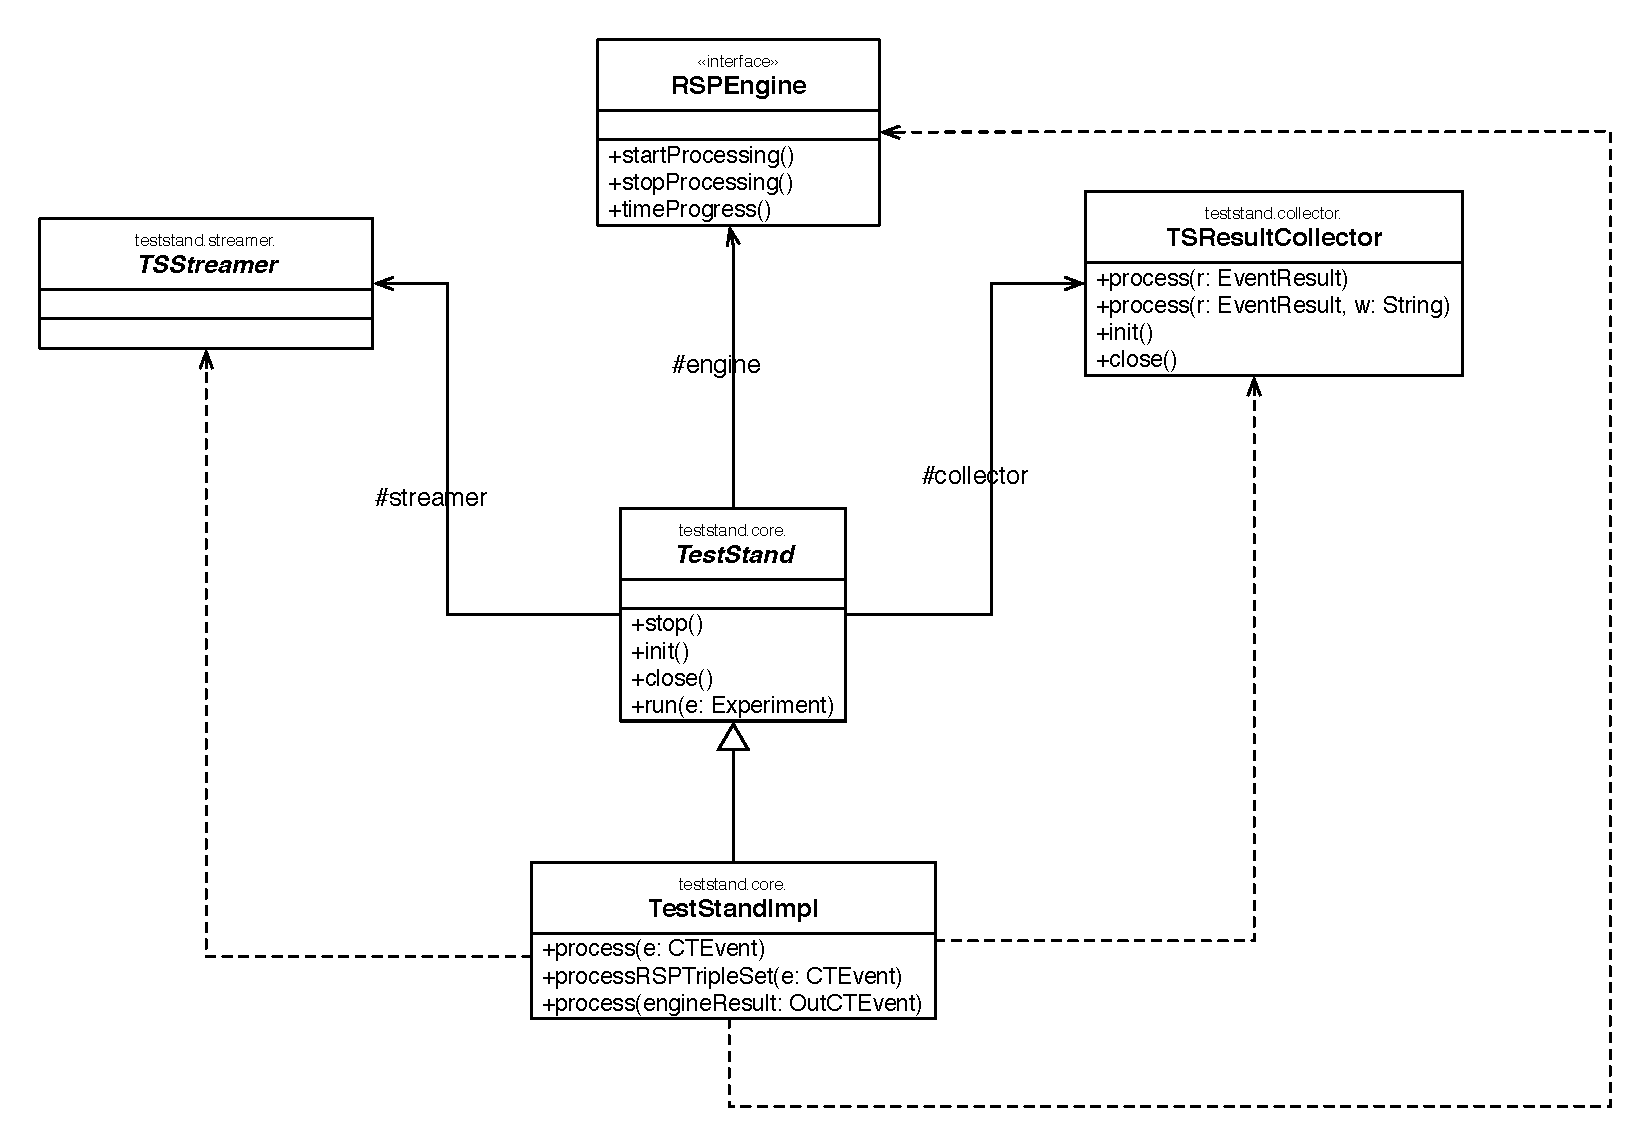
\includegraphics[width=0.9\linewidth]{images/uml_teststand_modules}
	\caption[\name \textsc{TestStand} and Modules  - UML Schema] {The \textit{TestStand} contains references of the \textit{TSStreamer}, the engine behind the \textit{RSPEngine} interface and the \textit{TSResultCollector}. The \textit{TSStreamer} and current \textit{RSPEngine} are linked to the next element in the pipeline trough the \textit{TestStand}. Two arrows, labelled with "next", point to the  \textit{TestStand} indicating that it receives the events from all modules and it orchestrates the communication. The arrow which start from the \textit{RSPEngine} is coloured in gray to highlight that it can not be seen at this level of detail, because \textit{RSPEngine} is an interface. The \textit{ResultCollector} receives the result to save at the end of each cycle, it does need a "next", because the process ends when it returns the call.} 
  	\label{fig:uml_teststand_modules}
\end{figure}

\pagebreak

\section{Baselines}\label{sec:baselines-impl}

\name Baselines are four elementary implementations of an RSP Engine, which  cover the requirements form [R.13] to [R.16] and implement the pipeline of a DSMS with a reasoner following the proposal presented in Section \ref{sec:baselines}. 
The RSP Engine pipeline is composed by Esper\footnote{$http://www.espertech.com/esper/$}, a mature commercial DSMS, with the Jena general purpose rule engine\footnote{http://jena.apache.org/documentation/inference/\#rules}, a flexible reasoning engine.  The aim of the choice of Esper and Jena is fulfilling requirement [R.14], baselines Eligibility by coupling two mature solutions for stream processing and reasoning to obtain a fair solution in the SR context.

\begin{figure}[tbh]
  \centering
	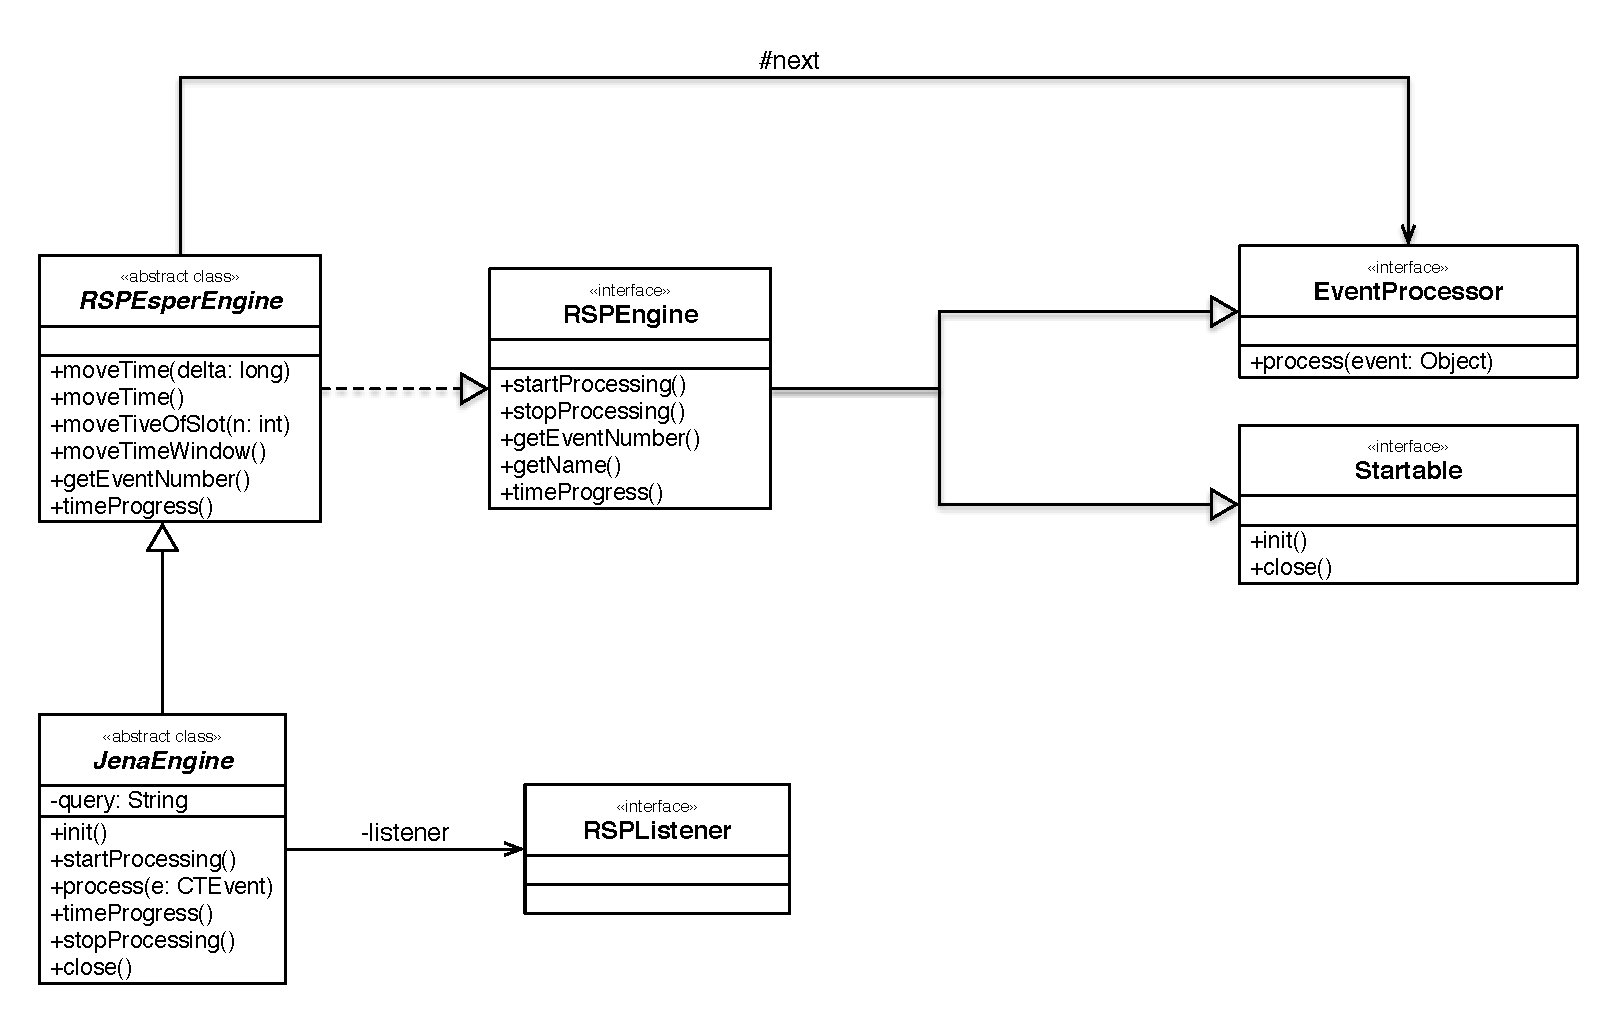
\includegraphics[width=\linewidth]{images/uml_baselines_general}
	\caption[\textit{RSPEngine} Implementation Trough Esper and Jena - UML Schema]{The \textit{RSPEngine} interface extends both the \textit{EventProcessor} and the \textit{Startable} ones. The \textit{RSPEsperEngine} class in picture implements the interface adding the Esper runtime to handle its internal events. The \textit{JenaEngine} together with the \textit{RSPListener} integrate the Jena reasoning system into the engine.}
  	\label{fig:uml_baselines_general}
\end{figure}

\noindent Figure \ref{fig:uml_baselines_general} presents how the baselines are implemented. The general structure exploits the \textit{RSPEngine} interface, a proxy for both the \textit{EventProcessor} and the \textit{Startable} interfaces described in Section \ref{sec:impl-intro} and in Section \ref{sec:modules-impl}. 

\name Baselines integrate Esper as the DSMS which compose the first half to the RSP Engine pipeline.  The \textit{RSPEsperEngine} abstract class implements the \textit{RSPEngine} interface in order to share the Esper runtime definition for all the Baselines.  They exploit the ability of Esper to be temporally controlled by an external agent\footnote{\url{http://esper.sourceforge.net/esper-0.7.5/doc/reference/en/html_single/index.html#api-controlling-time}}. Thus, the internal time flow can be synchronised by sending time-keeping events. In this way it possible to ensure the complete and soundness of query results, even in case of high traffic load. To enable external time control the \textit{RSPEngine} interface exposes the \textit{moveTime()} method.  The \textit{RSPEsperEngine} implements \textit{moveTime()} encapsulating the logic to send a time-keeping event into Esper: one time-keeping event is sent before injecting the triples within a \textsc{CTEvent} and the next one after all triples in \textsc{CTEvent} were sent. In this way all the triples in the \textsc{CTEvent} are consider contemporary by the Baselines. 

The RSP Engine is in the middle of the \textsc{Test Stand} pipeline, thus is has to communicate with the module below. The \textit{RSPEsperEngine} has a reference to a general \textit{EventProcessor}, represented in Figure \ref{fig:uml_baselines_general}  by the arrow labeled as "next", which can be any modules which processes \textit{CTEvent}. In the current implementation the \textsc{Test Stand External Structure}, implemented as the \textit{TestStandImpl} class, follows \textit{RSP Engine}, to intercept the outcoming\textit{OUTCTEvents}.

\begin{figure}[tbh]
  \centering
	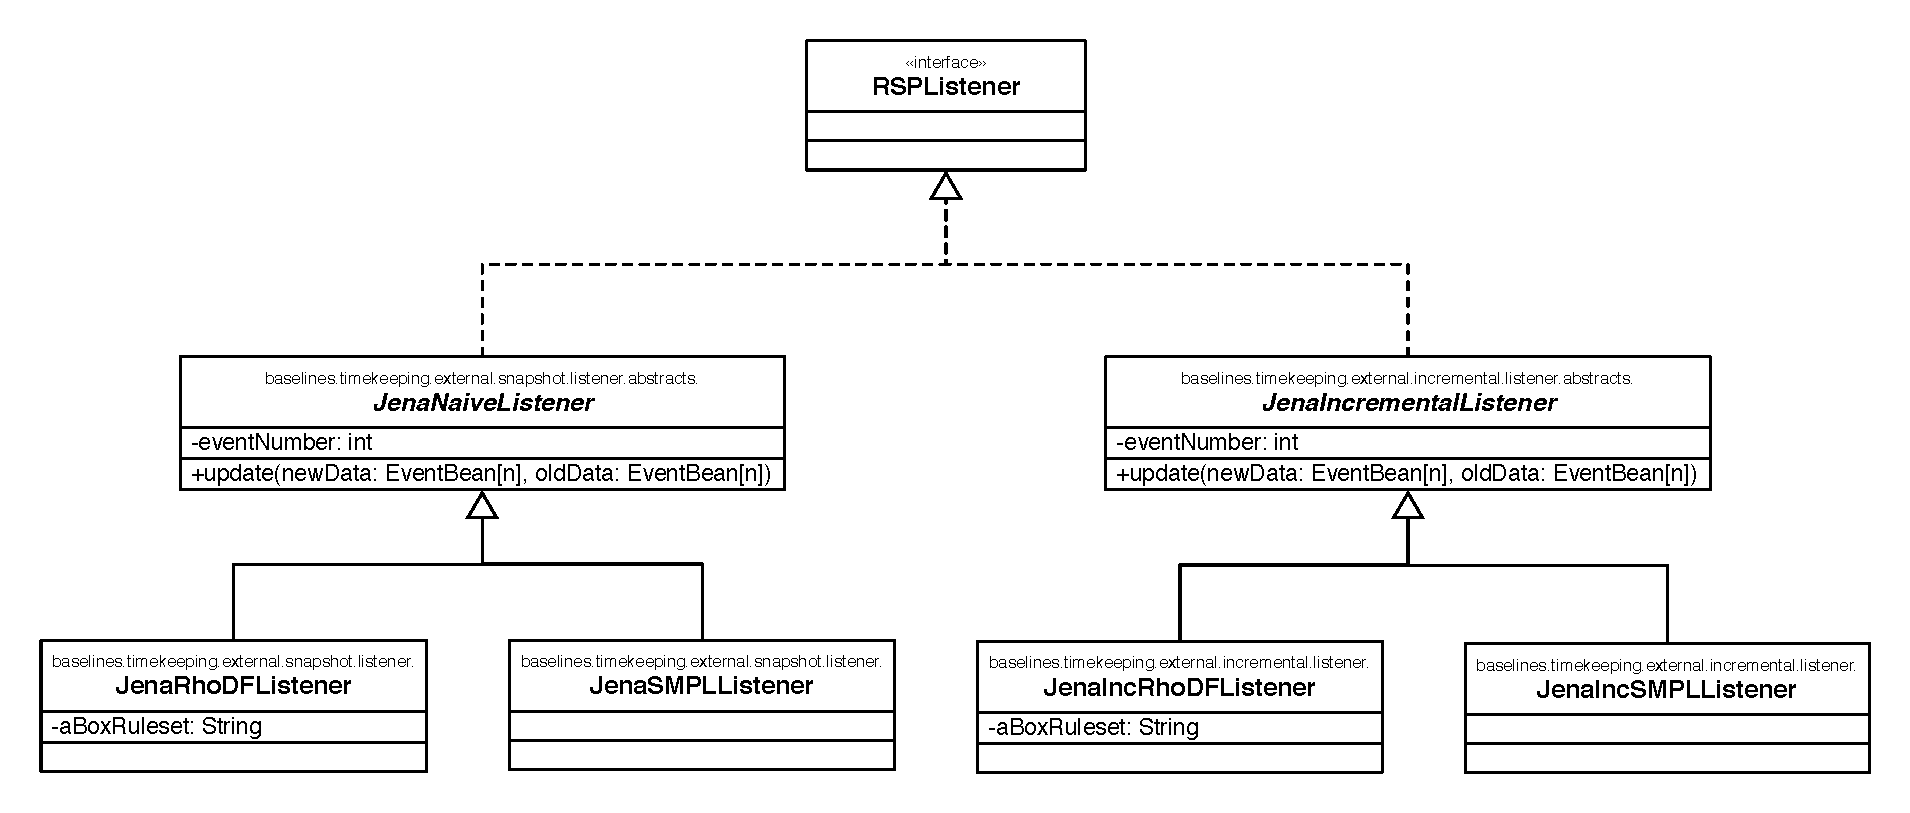
\includegraphics[width=\linewidth]{images/uml_baselines_listener}
	\caption[\textit{RSPListener} Implementations - UML Schema]{The \textit{RSPListener} is actually a proxy for the native Esper \textit{UpdateListener}. We implement the interface following two possible reasoning approaches, Naive and Incremental, respectively into the  \textit{JenaNaiveListener} and the \textit{JenaIncrementalListener}. Further implementations like the \textit{JenaNaive$\rho$DFListener} allows to specify the entailment regime and the TBox to the listeners.} 
  	\label{fig:uml_baselines_listener}
\end{figure}

We draw in Figure \ref{fig:uml_baselines_general} the UML schema of the Baseline implementation. The \textit{JenaEngine} abstract link the DSMS to the reasoner, an thus it requires a further component, the RSPListener, to complete the RSP Engine pipeline and realise the system we describe in Section \ref{sec:baselines}
 
The reasoner stage is realised as shown in Figure \ref{fig:uml_baselines_listener}. Different implementations of the listener, which all belongs to the the \textit{RSPListener} interface, variate the reasoning approaches between Naive or Incremental. The \textit{JenaNaiveListener} or the \textit{JenaIncrementalListener} partially fulfil requirement [R.15] (baseline relevance) in terms of reasoning. None of the two specify the entailment regime and the TBox, which must be defined with specific implementations like the \textit{JenaRHODFNaiveListener}, as it is visible again in the Figure \ref{fig:uml_baselines_listener}.

\begin{figure}[p!]
  \centering
	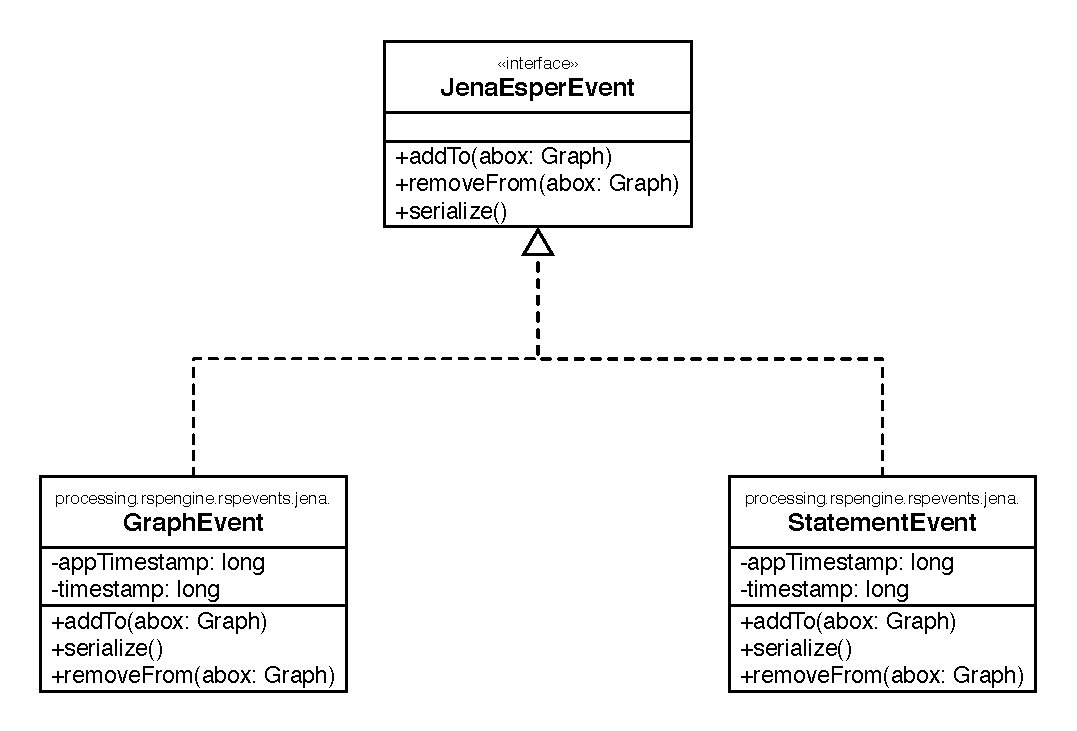
\includegraphics[width=0.8\linewidth]{images/uml_baselines_events}
	\caption[Esper-level Graph based and Triple based - UML Schema]{ All the event registered to Esper belong to the \textit{JenaEsperEvent} interface, which exposes methods to handle the reasoning independently from the RDF Stream implementation:  \textit{GraphEvent} or \textit{TripleEvent}. The triples received by the \textit{RSPEngine} can be pushed into Esper as complete graph or as a set statements. To handle the active window graph independently from the event implementation, the interface exposes the method \textit{addTo(Graph g)} and \textit{removeFrom(Graph g)}, while the \textit{serialise()} methods unroll the current event into a set of statement, in order to build an outgoing \textit{OutCTEvent}}
  	\label{fig:uml_baselines_events}
\end{figure}

The Baselines relevance demanded by [R.15] it is only partially fulfilled by the alternative reasoning approaches. It comes also from the different implementation of the RDFStream model, graph based or triple based. Esper runtime demands to registers the events that it has to handle. Figure \ref{fig:uml_baselines_events} shows how events are implemented: they belongs to the e \textit{JenaEsperEvent} interface, which exposes three methods used by the \textit{RSPListener} to manage the active window independently from event implementation. The methods \textit{addTo(Graph g)} and \textit{removeFrom(Graph g)} adelegates to the event the operations of insert and deletion to the event, in a transparent way for the \textit{RSPListener}; the method \textit{serialise()} unrolls the event into a set of statements, in this way the RSP Engine can output an \textit{OutCTEvent} independently from the RDF Stream implementation: \textit{GraphEvent} or \textit{TripleEvent}

Notice that when a \textit{CTEvents} comes to the RSP Engine it will be transformed into the events handled by the DSMS, contained in Figure \ref{fig:uml_baselines_events}. This translation process influences the latency calculus, because the time spent by the engine to translate events from the RDFStream into its internal mechanism may be relevant. Once the processing is complete, the output of the RSP Engine is translated again into an \textit{OutCTEvent} and passed to the next \textit{EventProcessor}, again spending time that influence the latency.

The current Baselines implementation divides the different architectural elements and delegates to each element a specific task to share the majority of the code and thus fulfilling [R.16], which demands baseline Simplicity.

%\begin{figure}[tbh]
%  \centering
%	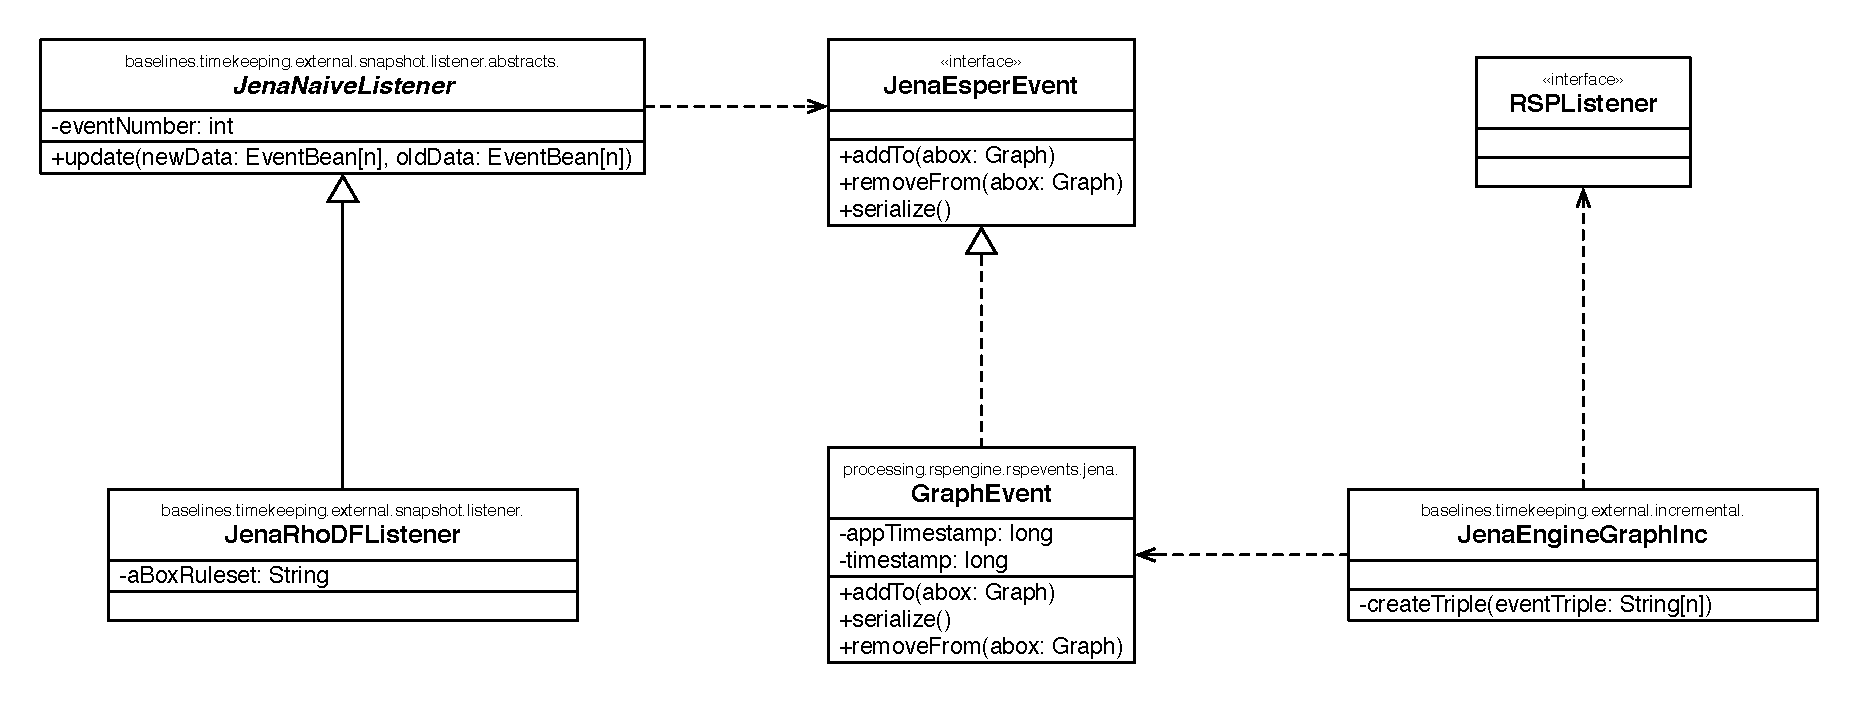
\includegraphics[width=\linewidth]{images/uml_baselines_rel_listener_event}
%	\caption[The Relation between \textit{RSPListener} and \textit{JenaEsperEvent} - UML Schema]{The listener and the event implementation are fully decoupled but logically related. In picture is detailed this relation for different implementation of the \textit{RSPListener}}
%  	\label{fig:uml_baselines_rel_listener_event}
%\end{figure}
%
%\textit{\textit{JenaNaiveListener} and the  \textit{JenaIncrementalListener} handle the events which come form the DSMS trough the \textit{JenaEsperEvent} interface, Figure \ref{fig:uml_baselines_rel_listener_event} report  the structure for the case of Graph-based event representation (see Section \ref{sec:baselines} for event details). }

\pagebreak

\section{Analyser}\label{sec:analyser-impl}

\begin{figure}[tbh]
  \centering
	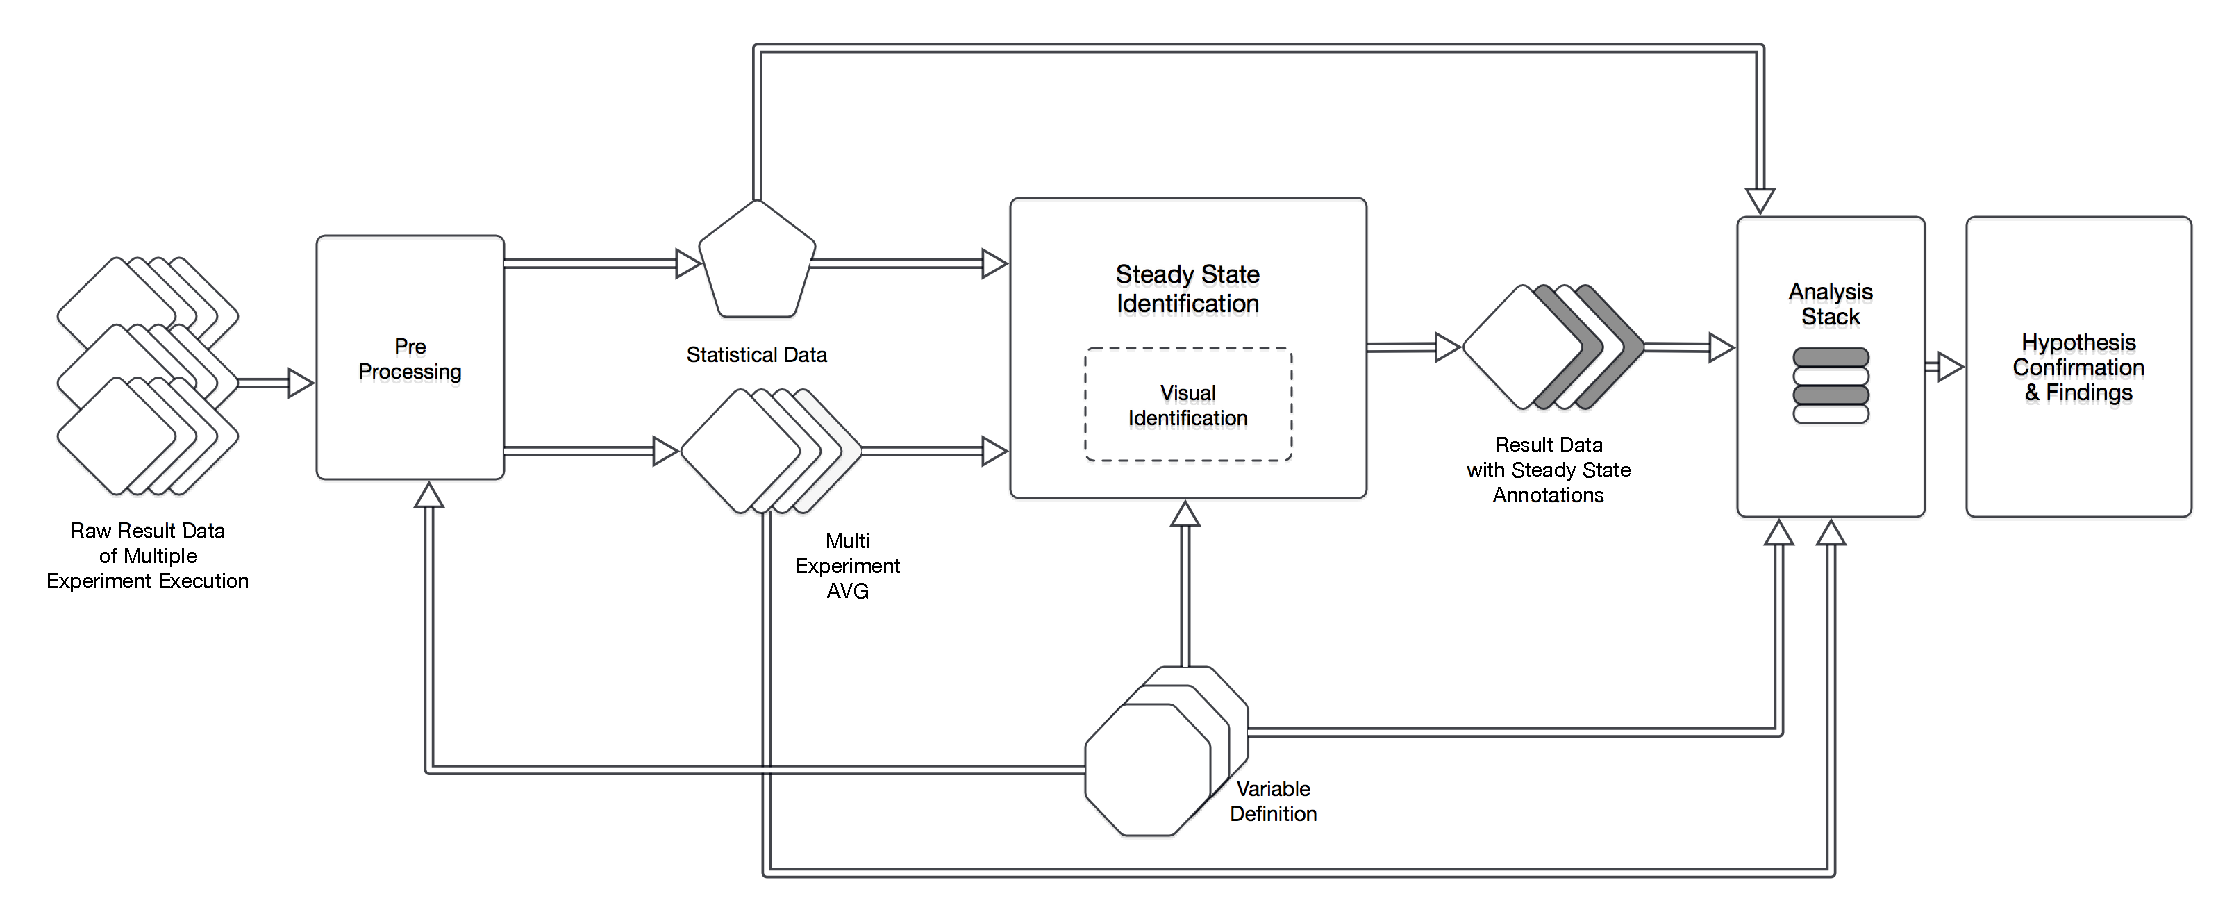
\includegraphics[width=\linewidth]{images/analyser-block-schema-impl}
	\caption[\textsc{Analyser} Block Schema: Implementation Detail Level]{The \textsc{Analyser} Block Schema in figure extends to the implementation detail the one of Figure \ref{fig:analyser-block-schema}. Differently from the previous schema, a new initial block, name Pre-Processing, operates on the experiment raw data in two ways: it averages among multiple execution of the same experiment, to obtain a single reliable dataset for each experiment; it calculates statistical relevant values for each experiment (maximum, minimum, median ecc). This module receives as input also the involved variables to design pre-processing, while its outputs are consumed by the following modules as the figure shows.}
  	\label{fig:analyser-block-schema-impl}
\end{figure}

\noindent In this section we introduce which analysis tools sustain the each level in the investigation stack described in Section \ref{sec:analyser} and how their realized in the current implementation of \name. Notice that the relation between the hypothesis and the tools that sustain the analysis is deep, thus it is hard to generalise the investigation toolset. Hypothesis depends on the the research question, while the tools are related to the nature of the data, which again concern the experiment.  However, there are some general meaningful characteristics, which are independent from both the hypothesis and experiment, that allow us to develop a basic toolset which sustains the entire investigation stack presented in Section \ref{sec:analyser}.

Figure \ref{fig:analyser-block-schema-impl} shows the different phases of data processing. It refers to the original block schema of drawn in Chapter \ref{chap:heaven}, but Figure \ref{fig:analyser-block-schema-impl} goes beyond the design level, providing some implementation details. 

The Figure \ref{fig:analyser-block-schema-impl} shows the \textsc{Analyser} receives two input:
\begin{itemize}
\item the raw data form the experiments
\item the variables to build the analysis
\end{itemize}


In the original block schema (See Figure \ref{fig:analyser-block-schema}) both inputs directly enter the \textit{Steady State Identification} Block (SSI) and the \textit{Analysis} Block (AB). In Figure \ref{fig:analyser-block-schema-impl}   instead, the first block in the process is the \textit{Pre-Processing Block}. Empirical analysis can not rely on a single execution of an experiment, because even if the \textit{Test Stand} is designed to be system independent, it remains a dynamic system. Thus, strange behaviours may happen while an experiment is running. In order to reduce and possible eliminate the outliers, multiple runs of the same experiment must be mediated obtaining the average measures The \textit{Pre-Processing} Block ensures data reliability extrapolating a unique dataset from multiple executions. Moreover, time series describes how a dynamic system evolves over time, so it is meaningful to attempt hypothesis verification trough statistical values, which always consider the the Steady State to allow the generalisation of the insights. The \textit{Pre-Processing} Block calculates most common statistical metrics as average , standard deviation and maximum or minimum for a certain variable.

%Indeed, both the Steady State Identification Block and Analysis Block require an automatic procedure, named pre-processing in Figure \ref{fig:analyser-block-schema-impl}, which averages the data of multiple executions of the same experiment and calculate the statistically relevant data. 

Once we have reliable data, the \textit{Steady State Identification} Block and the \textit{Analysis} Block receive them and start the analysis process. 

Finally, researches can read the analysis point out insight and theoretical results as the last block in the process describes.

Data mining procedures are very system-dependent. For this reason we include in Chapter \ref{chap:evaluation} about the \name Evaluation, concrete analysis examples, by testing the Baselines. The aim of Chapter \ref{chap:evaluation} is to demonstrate the value of \namens, but also we want to provide some guidelines for further evaluations.

The following subsections contains further details about the \textit{Steady State Identification} Block implementation, Subsection \ref{sec:analyser-impl-ss-block}, and about the \textit{Analyser} Block with the investigation stack, Subsection \ref{sec:analyser-impl-analysis-block}.

\subsection{Steady State Identification Block}\label{sec:analyser-impl-ss-block}

The Steady State Identification Block has the aim to  determines if a solution has reached the Steady State condition for a certain variable, as we describe in Section \ref{sec:analyser-analysis-block}. Automatic procedures to identify the State State condition exist, but they require dedicated studies which will be faced as future works. Currently, the SSI is not automated. It exploits data visualisation techniques, to identify, if and when Steady State condition is reached. Practically each variable in the system is plotted in the time domain over all the entire experiment and research can exclude  the initial warm-up phase form the data evaluation when that variables reaches a stable condition. 
We know that the graphical method is limited, because it must be applied for each system variable, and human criteria can nit be reliable in this kind of analysis as automatic procedures which exploits tested algorithms. Moreover, different variables may reach the equilibrium at different times, so it is researcher responsibility to properly identify the different condition for each variable involved.

\subsection{Analysis Block}\label{sec:analyser-impl-analysis-block}

\noindent The \textsc{Analyser} Design includes Five Analysis Levels (see Section \ref{sec:analyser} with increasing degrees of detail. The \textit{Analysis} Block hides the level where the comparative research approach is declined either to the visual analysis or statistical investigation. The graphical analysis method is more qualitative then the second one, but reading the information presented in graphical way can be preferred in those case where numerical data are not clear. On the other hand, the statistical investigation method demands more complex instruments to obtain the data, but allows to answer also elaborate questions with simpler answers. Following we present for all the Analysis level the method involved in the current implementation.

\subsubsection{Level 0 - Dashboards}\label{sec:impl-level0}

\begin{figure}[h!tbp]
  \centering
	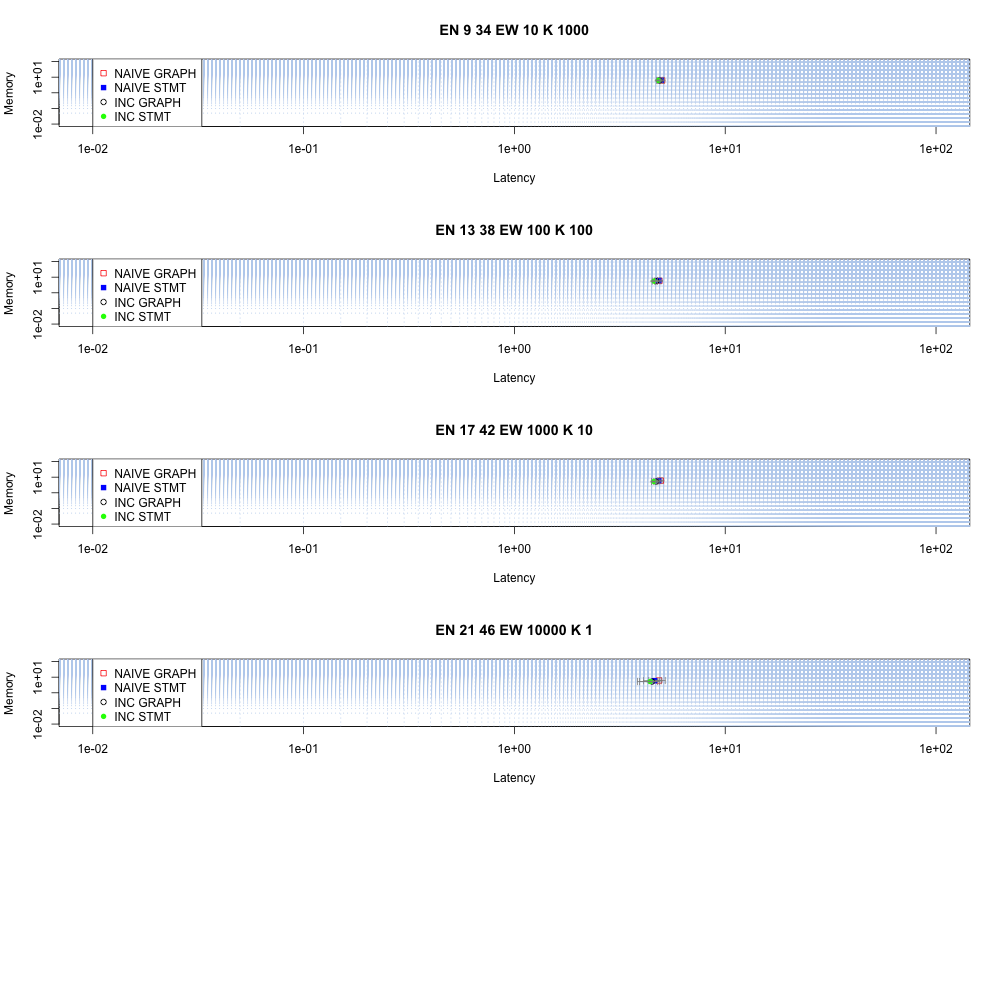
\includegraphics[width=0.45\linewidth]{images/dashboard-example}
	\caption[\textsc{Analyser} Investigation Stack - Level 0 -  Dashboard Representation Examples]{\textsc{Analyser} Investigation Stack - Level 0 -  Dashboard Representation Examples}
  	\label{fig:dashboard-example}
\end{figure}

\noindent Figure \ref{fig:dashboard-example} contains an example of the possible Dashboard representations. We implement the dashboard to represent data on a bi-dimensional Cartesian space where memory and latency are the axis of the graph. This kind of representation allows to define solution dominance, w.r.t the involved variable, trough inter-experiment comparisons. Thus, we can easily state which RSP Engine, if any, is better then another one looking to a dashboard.

\subsubsection{Level 1 - Statistical Values Comparison}\label{sec:impl-level1}

Tables \ref{tab:comp-tables} (a) and (b) show two examples of statistical investigation. Table \ref{tab:comp-tables}.a contains the qualitative comparison of two solution over a given variable, while Table \ref{tab:comp-tables}.b offers a deeper details level, the quantitative comparison, showing how much a solution is better than the other. How to choose the proper level depends on the needs of the research.

\begin{table}[htb]
\scriptsize
	\centering
	\subtable[Symbolic Comparison of variables A vs B on Experiment 1]{%
		\begin{tabular}{c | cccc} % creating eight columns
	  	\hline
		A vs B & \multicolumn{4}{c}{Experiment 1 Condition A}  \\
		 Comparison  & &&&\\
		\hline
		   	        & $\simeq$\\
		 Experiment 1 & A     & 	$\simeq$  & A & B\\
		 Condition  & A     & 	$\simeq$  & $\simeq$ & B\\
		 B          & A     & 	$\simeq$  & B & A\\
		\hline % inserts single-line
	 \end{tabular}
	}\qquad\qquad
	\subtable[Symbolic Comparison of variables A vs B on Experiment 1]{%
		\begin{tabular}{c | cccc} % creating eight columns
	  	\hline
		A vs B & \multicolumn{4}{c}{Experiment 1 Condition A}  \\
		 Comparison  & &&&\\
		\hline
		   	        & $\simeq$\\
		 Experiment 1 & 10\%     & 	$\simeq$  & 42\% & 33\%\\
		 Condition  & 23\%     & 	$\simeq$  & $\simeq$ & 12\%\\
		 B          & 20\%    & 	$\simeq$  & 22\% & 22\%\\
		\hline % inserts single-line
	 \end{tabular}
	}
	\caption[\textsc{Analyser} Investigation Stack - Level 1 - Qualitative and Quantitative Comparison Examples]{\textsc{Analyser} Investigation Stack - Level 1 - Example of qualitative-comparison over two variables  (a)  and  quantitative-comparison over a common variable (b) }
	\label{tab:comp-tables}
\end{table}

Table layout is a key-point for Level 1 representations. Tables axes represent the variation of two different experiment properties A and B. Different experiments influence the behaviour of an RSP Engine in different ways, and Level 1 allows to point out this differences with  \textit{Inter-Experiment} comparisons. Thus, we can move on the horizontal axis of Table \ref{tab:comp-tables}.a, which means variate the Condition A, to appreciate those differences. 

Actually this kind of analysis is possible thanks to a CSV report, which contains all the meaningful statistical values for the experiments. The report can be further manipulated to obtain the table visualisation.

\subsubsection{Level 2 - Patter Identification}\label{sec:impl-level2}

%\begin{figure}[tbh]
%  \centering
%   \subfigure[Pattern Recognition Example: Memory in Time Domain]{
%  	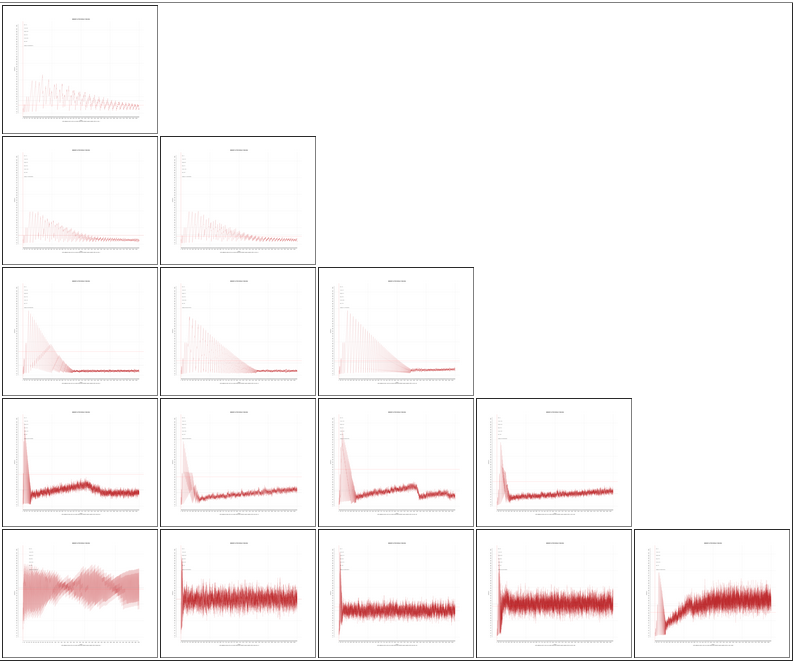
\includegraphics[width=0.45\linewidth]{images/pattern-example-memory}
%  }
%  \subfigure[Pattern Recognition Example: Memory Distribution]{
%  	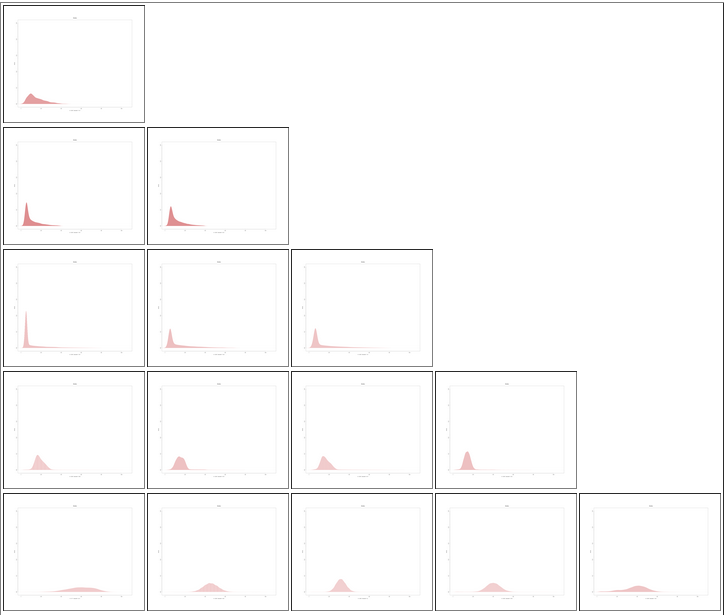
\includegraphics[width=0.45\linewidth]{images/pattern-example-density}
%  	
%  }
%   %\subfigure[Pattern Appear On the Wall..]{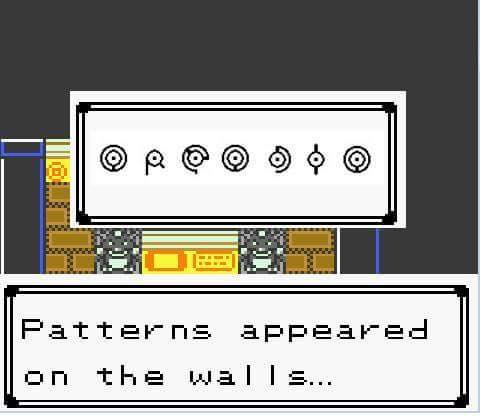
\includegraphics[width=0.45\linewidth]{images/pokepattern}}
%	\caption[\textsc{Analyser} Investigation Stack - Level 2 - Pattern Recognition Examples]{Two examples of pattern recognition. Level 2 exploits  easy-to-read layouts which highlights the experiment difference to enable \textit{Inter Experiment} comparisons} 
%  	\label{fig:pattern-examples}
%\end{figure}

\begin{table}[htbp]
	\centering
	\scriptsize
	\subtable[Pattern Recognition Example: Memory Time Domain]{%
		\begin{tabular}{l | ccccc} % creating eight columns
	  	\hline
		Triple  & \multicolumn{5}{c}{Slots}  \\
		in & \multicolumn{5}{c}{Number}  \\
		Window  & 1 & 10 & 100 & 1000&10000\\
		\hline
		1	   &\begin{minipage}{.1\textwidth}
     			 	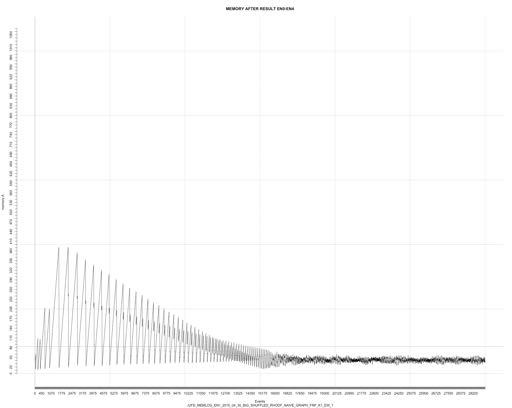
\includegraphics[width=\linewidth]{images/mema-graph/N1}
    				 \end{minipage}\\			
		10	   & \begin{minipage}{.1\textwidth}
     			 	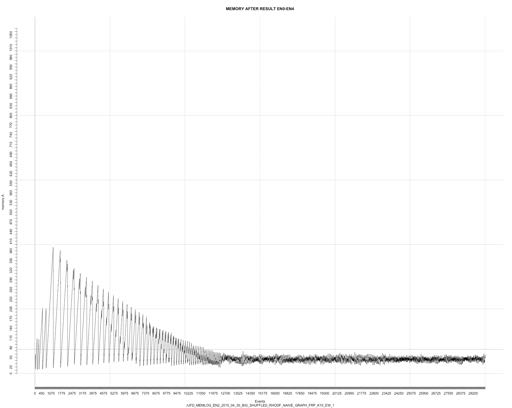
\includegraphics[width=\linewidth]{images/mema-graph/N2}
    				\end{minipage}
    			   & \begin{minipage}{.1\textwidth}
     			 	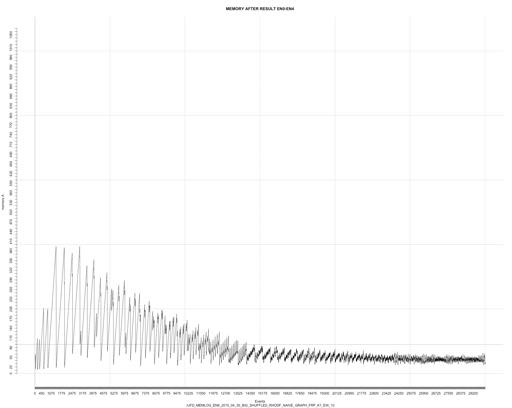
\includegraphics[width=\linewidth]{images/mema-graph/N6}
    				 \end{minipage}\\		
		100	   & \begin{minipage}{.1\textwidth}
     			 	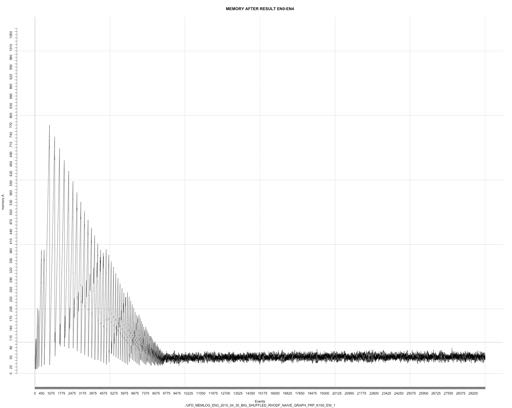
\includegraphics[width=\linewidth]{images/mema-graph/N3}
    				 \end{minipage}
    			   & \begin{minipage}{.1\textwidth}
     			 	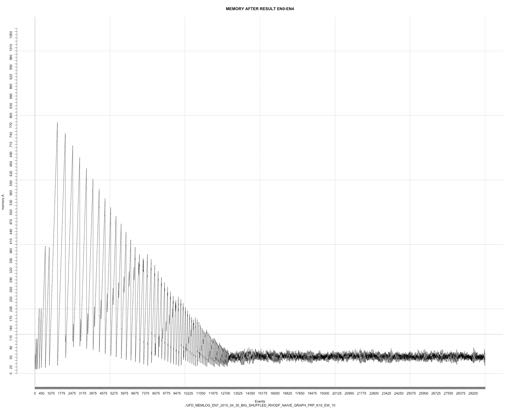
\includegraphics[width=\linewidth]{images/mema-graph/N7}
    				 \end{minipage}
    			   &	 \begin{minipage}{.1\textwidth}
     			 	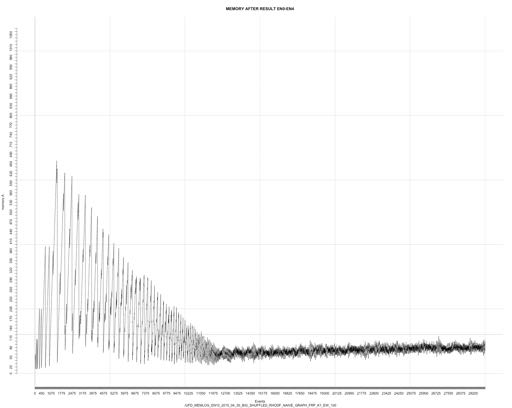
\includegraphics[width=\linewidth]{images/mema-graph/N10}
    				 \end{minipage}\\	
		1000   &	 \begin{minipage}{.1\textwidth}
     			 	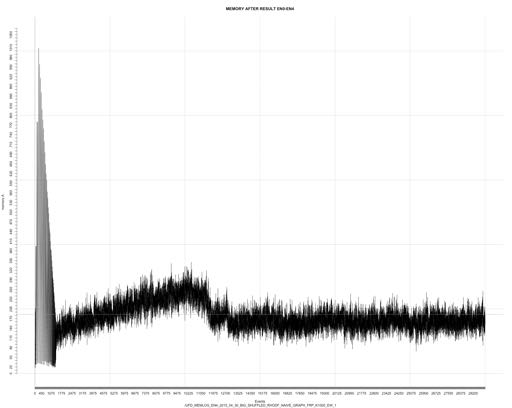
\includegraphics[width=\linewidth]{images/mema-graph/N4}
    				 \end{minipage}
    			   &	 \begin{minipage}{.1\textwidth}
     			 	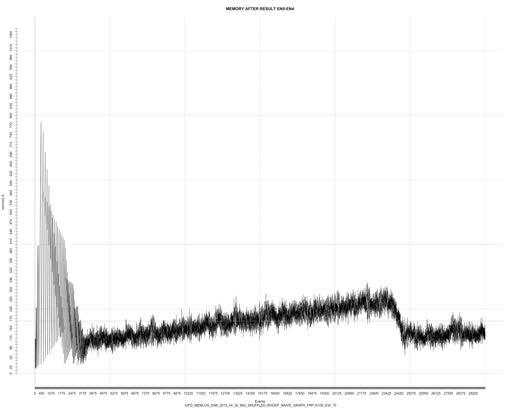
\includegraphics[width=\linewidth]{images/mema-graph/N8}
    				 \end{minipage}
    			   &	 \begin{minipage}{.1\textwidth}
     			 	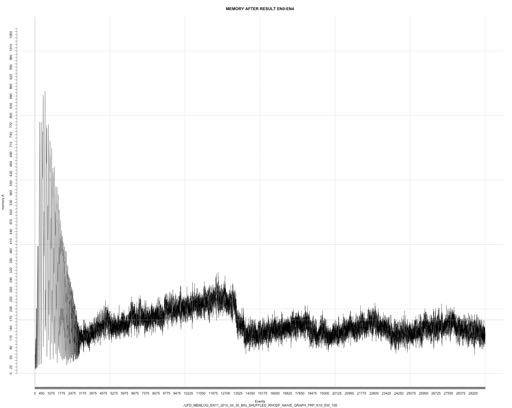
\includegraphics[width=\linewidth]{images/mema-graph/N11}
    				 \end{minipage}
    			   &	 \begin{minipage}{.1\textwidth}
     			 	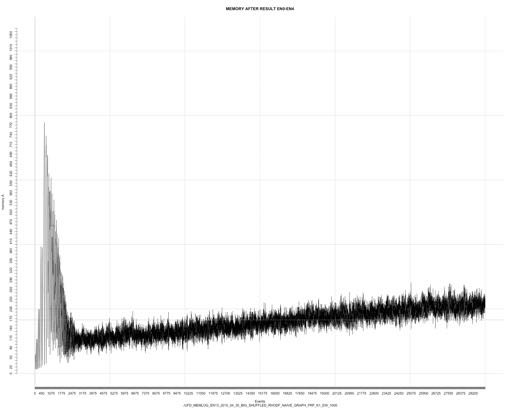
\includegraphics[width=\linewidth]{images/mema-graph/N13}
    				 \end{minipage}\\
		10000  &	 \begin{minipage}{.1\textwidth}
     			 	
\includegraphics[width=\linewidth]{images/mema-graph/N5}
    				 \end{minipage}
    			   &	 \begin{minipage}{.1\textwidth}
     			 	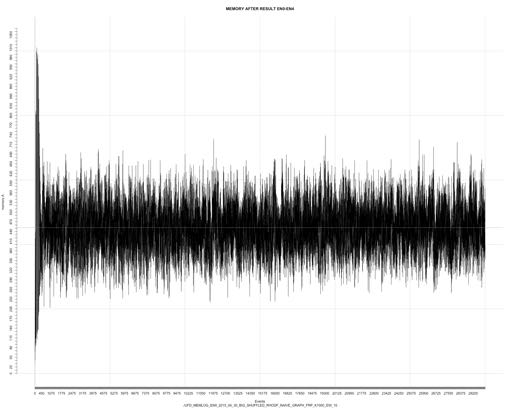
\includegraphics[width=\linewidth]{images/mema-graph/N9}
    				 \end{minipage}
    			   &	 \begin{minipage}{.1\textwidth}
     			 	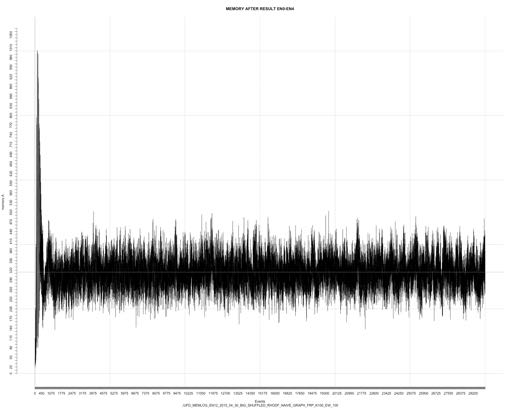
\includegraphics[width=\linewidth]{images/mema-graph/N12}
    				 \end{minipage}
    			   &	 \begin{minipage}{.1\textwidth}
     			 	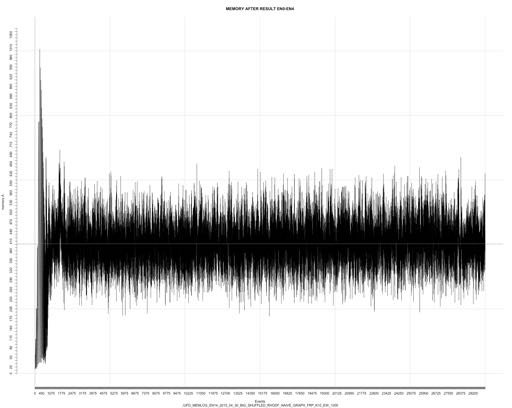
\includegraphics[width=\linewidth]{images/mema-graph/N14}
    				 \end{minipage}
    			   &	 \begin{minipage}{.1\textwidth}
     			 	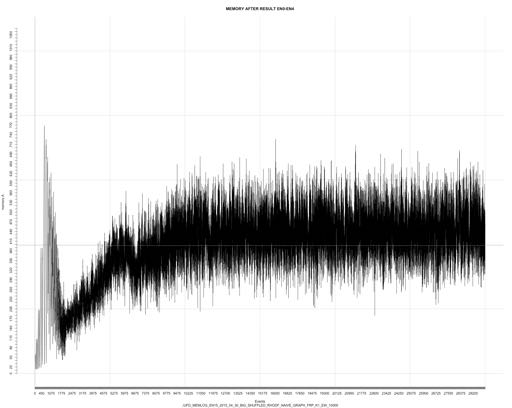
\includegraphics[width=\linewidth]{images/mema-graph/N15}
    				 \end{minipage}\\
		\hline % inserts single-line
	 \end{tabular}
	}
	\subtable[Pattern Recognition Example: Memory Distribution]{%
		\begin{tabular}{l | ccccc} % creating eight columns
	  	\hline
		Triple  & \multicolumn{5}{c}{Slots}  \\
		in & \multicolumn{5}{c}{Number}  \\
		Window  & 1 & 10 & 100 & 1000&10000\\
		\hline
		1	   &\begin{minipage}{.1\textwidth}
     			 	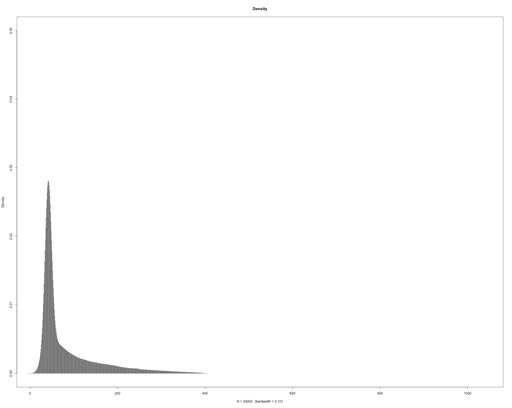
\includegraphics[width=\linewidth]{images/mema-dens-graph/N1}
    				 \end{minipage}\\			
		10	   & \begin{minipage}{.1\textwidth}
     			 	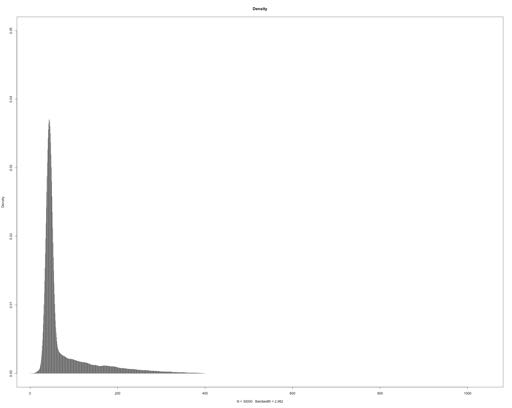
\includegraphics[width=\linewidth]{images/mema-dens-graph/N2}
    				\end{minipage}
    			   & \begin{minipage}{.1\textwidth}
     			 	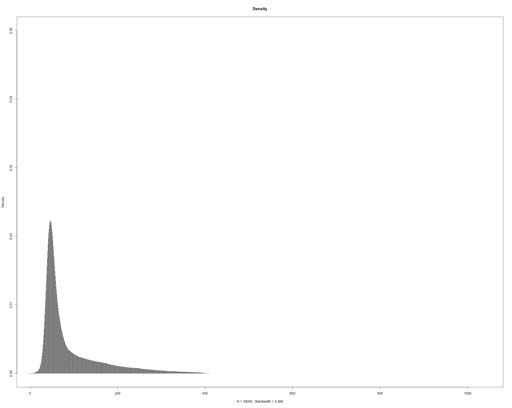
\includegraphics[width=\linewidth]{images/mema-dens-graph/N6}
    				 \end{minipage}\\		
		100	   & \begin{minipage}{.1\textwidth}
     			 	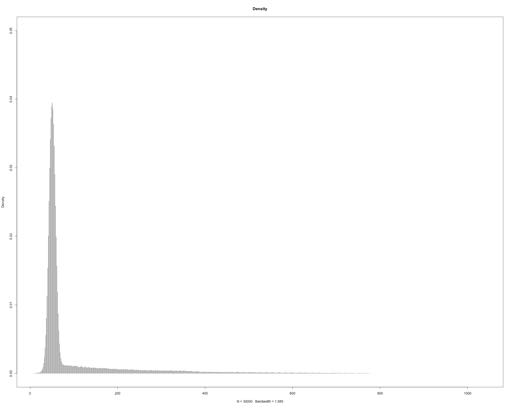
\includegraphics[width=\linewidth]{images/mema-dens-graph/N3}
    				 \end{minipage}
    			   & \begin{minipage}{.1\textwidth}
     			 	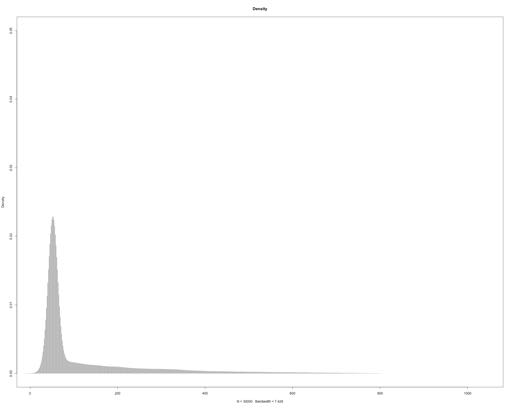
\includegraphics[width=\linewidth]{images/mema-dens-graph/N7}
    				 \end{minipage}
    			   &	 \begin{minipage}{.1\textwidth}
     			 	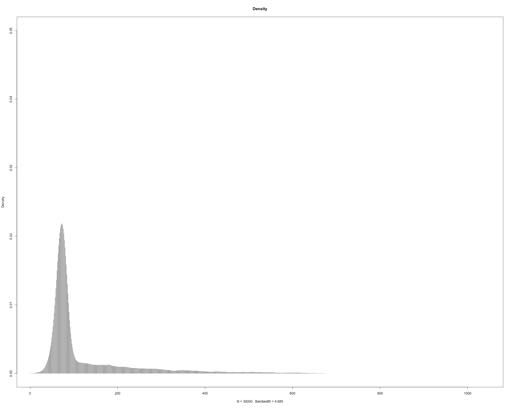
\includegraphics[width=\linewidth]{images/mema-dens-graph/N10}
    				 \end{minipage}\\	
		1000   &	 \begin{minipage}{.1\textwidth}
     			 	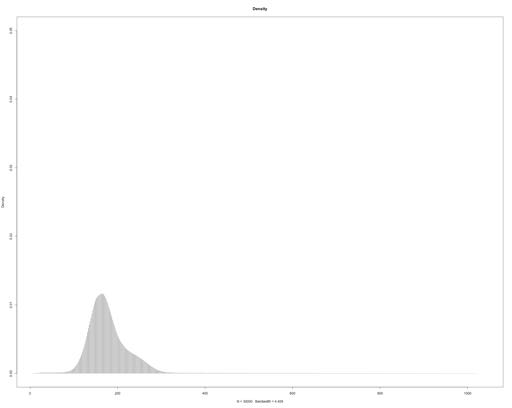
\includegraphics[width=\linewidth]{images/mema-dens-graph/N4}
    				 \end{minipage}
    			   &	 \begin{minipage}{.1\textwidth}
     			 	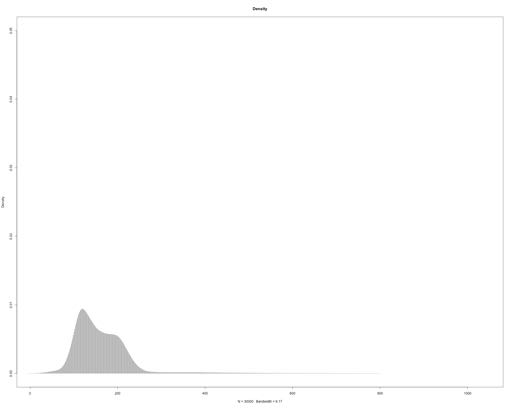
\includegraphics[width=\linewidth]{images/mema-dens-graph/N8}
    				 \end{minipage}
    			   &	 \begin{minipage}{.1\textwidth}
     			 	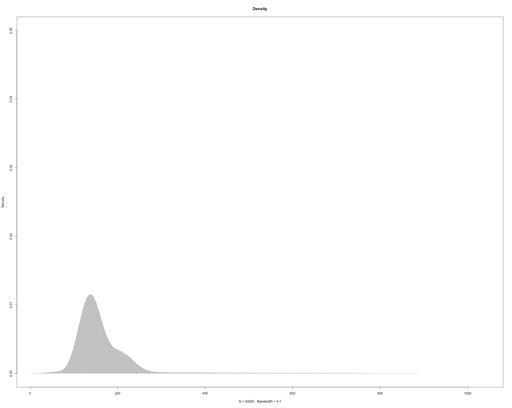
\includegraphics[width=\linewidth]{images/mema-dens-graph/N11}
    				 \end{minipage}
    			   &	 \begin{minipage}{.1\textwidth}
     			 	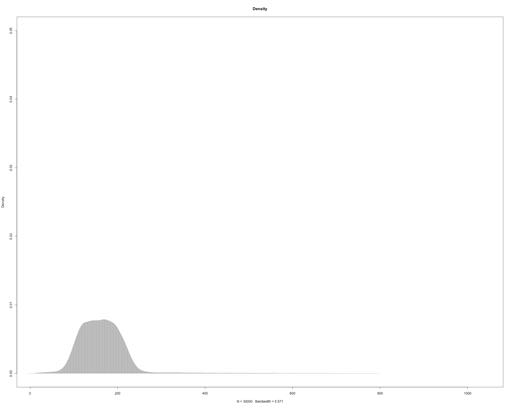
\includegraphics[width=\linewidth]{images/mema-dens-graph/N13}
    				 \end{minipage}\\
		10000  &	 \begin{minipage}{.1\textwidth}
     			 	\includegraphics[width=\linewidth]{images/mema-dens-graph/N5}
    				 \end{minipage}
    			   &	 \begin{minipage}{.1\textwidth}
     			 	\includegraphics[width=\linewidth]{images/mema-dens-graph/N9}
    				 \end{minipage}
    			   &	 \begin{minipage}{.1\textwidth}
     			 	\includegraphics[width=\linewidth]{images/mema-dens-graph/N12}
    				 \end{minipage}
    			   &	 \begin{minipage}{.1\textwidth}
     			 	\includegraphics[width=\linewidth]{images/mema-dens-graph/N14}
    				 \end{minipage}
    			   &	 \begin{minipage}{.1\textwidth}
     			 	\includegraphics[width=\linewidth]{images/mema-dens-graph/N15}
    				 \end{minipage}\\
		\hline % inserts single-line
	 \end{tabular}
	}
	\caption[\textsc{Analyser} Investigation Stack - Level 2 - Pattern Recognition Examples]{Two examples of pattern recognition. Level 2 exploits  easy-to-read layouts which highlights the experiment difference to enable \textit{Inter Experiment} comparisons} 
	\label{tab:pattern-examples}	
\end{table}

\noindent Level 2 exploits the same experiment layout of Level 1 to compare many graphical representation of the experiment variable. Two examples of memory analysis at Level 2 are reported in Tables \ref{tab:pattern-examples} (a) and (b). Table \ref{tab:pattern-examples}.a show the memory behaviour in time domain. It allows answer questions like "How the system changes the memory behaviour changing the input dimension?". Table \ref{tab:pattern-examples}.b reports the distribution memory values upon several intervals. It allows to understand how memory distribution is influenced by changing the variable on the Table axes or diagonals.

Level 3 aims of pattern identification for a given variable in an experimental set. It is an example of \textit{Inter-Experiment} comparison which enable a new kind of global analysis, because it requires to state observation upon the entire set of experiment.

\subsubsection{Level 3 - Visual Comparison}\label{sec:impl-level3}

\noindent Finally, Level 3 focuses on single graphical visualisation. Figure \ref{fig:visual-comp} contains two examples of the possible analysis. Figure \ref{fig:visual-comp}.a shows a case of \textit{Inter Experiment}comparison, highlighting the relation between the same variable over multiple experiments; Figure \ref{fig:visual-comp}.b provides an example of \textit{Intra Experiment} comparison, highlighting the relation between memory and latency within the same experiment.

\begin{figure}[tbh]
  \centering
  \subfigure[Multi-Experiment Comparison]{
  			\includegraphics[width=0.70\linewidth]{images/comp-inter}
  			}
  \subfigure[Multi-Variables Comparison]{
  \includegraphics[width=0.70\linewidth]{images/comp-intra}
  }
\caption[\textsc{Analyser} Investigation Stack - Level 3 - Visual Comparison Examples]{\textsc{Analyser} Investigation Stack - Level 3 - Figure (a) shows a case of \textit{Inter Experiment} visual comparison of the memory usage while Figure (b) present a case of \textit{Intra Experiment} comparison of latency and memory.}
  \label{fig:visual-comp}
\end{figure} \clearemptydoublepage
%The goal of this Chapter is to show how \name can improve the traditional top-down analysis method. Usually, researchers start from a deep comprehension of the theoretical problem  to to draw a model of the system over which is possible to formulate hypothesis. Further knowledge about  the implementation experience may support this method, however this approach is traditionally top-down. In this chapter we present an evaluation of \name Baselines (See Chapter \ref{sec:baselines}) in order to demonstrate how \name can extend the traditional hypothesis-based research towards the Systematic Comparative Research approach we introduced in Chapter \ref{chap:problem-settings}. Firstly, in section \ref{sec:experimental-setting} we describe the Experimental Setting, presenting our assumptions and two experiment sets for baselines evaluation. With the SOAK Test, in Section \ref{sec:soak-es}, we follow the traditional research method, showing its limitations with empirical results. In Section \ref{sec:step-es} we extends the research work on the baselines as an example of \name potential.

\section{Experimental Setting}
\label{sec:experimental-setting}

It is hard to formulate and prove hypothesis which are only based on he knowledge of the a model. The purpose of these tests is to show why is difficult to reach results trough this method, even for simple hypothesis, and consequently demonstrate that we need \namens .

The experimental setting of the evaluation consist in all the assumptions and the convention we have decided before starting the evaluation, in order to reach our goal. Practically, the experimental setting  consists into the definition of different tests to cover the most important variations on the tuple presented in Chapter \ref{chap:heaven}, which describes an experiment as $<\mathcal{D}, \mathcal{T},\mathcal{E}, \mathcal{Q}>$, where:
\begin{itemize}
\item $\mathcal{E}$ is the RSP Engine
\item $\mathcal{D}$ is the Dataset 
\item $\mathcal{T}$ is the Ontology
\item $\mathcal{Q}$ is the Query that $\mathcal{E}$ continuously answers.
\end{itemize}



The reason why we chose the Baselines as the RSP Engines $\mathcal{E}$ subject of our experiment is that Top-Down investigations are harder for commercial solutions like C-SPARQL Engine and CQELS. The the complexity of the architecture of these commercial solutions is high, and can not be easily faced in order formulate hypothesis of comparison. For the baselines instead this survey is possible. We have a complete model of their system and we also know many implementation details that can help during the analysis. Moreover,  in Chapter \ref{chap:problem-settings} we describe which requirements guarantee that an RSP Engine is a baselines (SERE properties): Simplicity, Elementarily, Relevance and Eligibility allow us to evaluate the baselines as a simple term of comparison for further research on Stream Reasoning systems and they clarify how to develop the investigation.
 
Section \ref{sec:baselines} shows that the four baselines differ for two characteristics: RDF Stream Model and Reasoning architecture. The Table \ref{tab:baselines-names} summarises these few but well determined differences, naming the four baselines for the evaluation:\begin{table}[htb]
\scriptsize
\centering
\begin{tabular}{c|cc} % creating eight columns
	\hline
         & Naive & Incremental\\
	\hline
	Graph        &  B1      & B2\\
	Statment   &  B3   & B4\\
	\hline % inserts single-
\end{tabular}
\caption{Configuration of the four baselines}
\label{tab:baselines-names}
\end{table}

\noindent Among these four configurations we formulate simple hypothesis, stating which approach is better then an other one within an experiment. How we realised the baselines is described in Section \ref{sec:baselines-impl}; the know-how about their internal mechanisms may help to find the motivations behind behaviours which are unpredictable form the architectural viewpoint. 

The Dataset  $\mathcal{D}$ and the Ontology $\mathcal{T}$ must be chose to ensure baselines Simplicity, as stated in Section \ref{sec:baselines}. We take $\rho$DF  \cite{DBLP:conf/esws/MunozPG07} as their entailment regime, because several works in the field \cite{DBLP:conf/semweb/UrbaniMJHB13} choose this as the minimal meaningful task for a Stream Reasoner. In particular, $\rho$DF is the RDF-S fragment that reduce complexity while preserving the normative semantics and core functionalities. 

The RDF streams  $\mathcal{D}$ used in the experiments are obtained streaming in different ways the data generated with LUBM  \cite{Guo2005} and the ontology $\mathcal{T}$ is the LUBM one\footnote{http://swat.cse.lehigh.edu/onto/univ-bench.owl}. We assume that the ontology does not change over time, therefore the materialisation of $\mathcal{T}$ is computed before starting the experiment and the RSP engine does not have to perform this task. It is worth to discuss the choice of using data from LUBM over SRbench and LSbench. The first one has data, which are not adequate for the experiments, since they do not require any reasoning. The SRbench data, on the contrary, requires reasoning, but, being real-data, do not have the possibility to be scaled up and down. This choice accomunate us to previous works on Stream Reasoning \cite{DBLP:conf/semweb/UrbaniMJHB13}. 

The data generator system, responsible to build $\mathcal{D}$ w.r.t. $\mathcal{T}$, is able to scale both in terms of dimension of the dataset and the reasoning effort. Being LUBM static data, we exploit the \textit{RDF2RDFStream} component of the test stand that takes care to adapt the data generate by LUBM to a streaming scenario. The component can be set up to obtain an RDFStream where the number of triples with the same timestamps follows a given discrete function, Section \ref{sec:streamer-impl} contains the implementation details of this particular \textsc{Streamer}. %e' veramente il timestamp quello?

The experiments in this Section are thought to show what kind of testing is possible trough \namens. We designed two kind of experiments based on the \textit{RDF2RDFStream} capabilities to control the triple distribution in the RDFStream. In order to evidence system dynamics over a particular input both the experiment typologies belong to the category of Stress Test:
\begin{itemize}
\item \textbf{SOAK}: the number of contemporary triple in the RDFStream does not change during the experiment.
\item \textbf{Step Response} the number of contemporary triple suddenly changes during the experiment, usually increasing of a degree of magnitude.
\end{itemize}
 
Finally, the queries $\mathcal{Q}$, used in the experiments, are variants of the same two basic identity queries that continuously asks for the materialisation of the current window:
\begin{enumerate}
\item[Q.1] Naive
\item[Q.2] Incremental
\end{enumerate}
 		 
Q.1 outputs the snapshot of the entire window and it is used for the Naive reasoning approach; Q.2 outputs the ir-streams and it is used for the Incremental reasoning approach. The queries differ for the size $\omega$ of the sliding window. In particular, we use windows in which $\omega$ is an integer multiple of the slide parameter $\beta$ of the window, i.e., it holds that $\omega = \beta * N$. In other words, $N$ is the number of \textsc{CTEvents} that the window contain. 

Moreover, Section \ref{sec:baselines-impl} shows how the proposed baselines take advantage of the ability of Esper to be temporally controlled by an external agent\footnote{\url{http://esper.sourceforge.net/esper-0.7.5/doc/reference/en/html_single/index.html#api-controlling-time}} by sending time-keeping events to synchronise the internal time flow. All the triples in the \textit{CTEvent} are consider contemporary by the baselines and each \textit{CTEvent} can be seen as a proxy for the timing event. Together with the \textit{RDF2RDFStream} is possible to estimate the content of the current window in terms of number of RDF Triples in any moment of the experiment.\\

Following we describe in details the content of the SOAK (Section \ref{sec:soak-es}) and the Step Response tests (Section \ref{sec:step-es}), providing a lecture key for the experiment results.

\section{Experiment Design}

Experiment design has the goal to prove one or more hypothesis, evidencing the behaviour of the system in the context that those hypothesis involves. Experiment design starts with some assumptions, for example in Section \ref{sec:experimental-setting} we explain the reasons why we chose $\rho$DF as entailment regime for our experiments. Researchers formulate hypothesis on the base of these assumption, and they design experiments to verify hypothesis validity. Figure \ref{fig:experiment-design} summarises this approach.

\begin{figure}[tbh]
  \centering
	\includegraphics[width=\linewidth]{images/experiment-design}
	\caption{Traditional Experiment design workflow} 
  	\label{fig:experiment-design}
\end{figure}


From a theoretical point of view we decide to study RSP Engine facing their nature of linear dynamic system. Experiment design also require to point out which variable are observed. We simplify the study analysing their behaviour in term of Latency and Memory, as reported in Chapter \ref{chap:heaven}, and comparing the results of the four baselines (see Table \ref{tab:baselines-names}) between many experiments.

\subsection{SOAK: Tests and Hypothesis}\label{sec:soak-es}

Soak testing show the system dynamics, stressing the subject with a constant and continuous input flow. In the Stream Reasoning context the RDFStream is controlled to have the same number of contemporary triple over time. 

All the experiments are 20000 events long, this duration ensures to reach for majority of the experiments the Steady State condition for both latency and the memory. Unlikely, is not possible to foretell how many events are required in to reach the Steady State condition for a certain variable, especially memory. Multiple attempts and empirical evaluation are the only way to set up the correct longness. All experiment are executed 10 times, and we take the average to reduce measurement error. 

\begin{table}[htb]
\centering
 \begin{tabular}{l|c| lllll}
	  	\hline
		\multicolumn{2}{c|}{  } &\multicolumn{5}{c}{Window size}  \\
		\multicolumn{2}{c|}{  } & 1 & 10 & 100 &1000 &10000\\
		\hline
		\hline
		 & 1 & 1 & 10 & 100 & 1000&10000 \\
		\textsc{CTEvent}      & 10  & 10  & 100  & 1000 & 10000  \\
		size             &100   & 100   & 1000 & 10000  \\
					&1000   & 1000 & 10000 \\
					&10000   & 10000  \\
		\hline 
	\end{tabular}
	
	 \vspace{10pt}
	\caption{The number of triples in the window during the ten SOAK tests as a function of the Window size (in terms of $N$) and of the triples in each \textsc{CTEvent}.}
	\label{tab:soaktests}
\end{table}

Table \ref{tab:soaktests} presents the fifteen SOAK tests we run for each baseline presented in Table \ref{tab:baselines-names}. The columns of the table are the different window sizes measured in terms of the values assumed by $N$.  Being $\beta=$ 100 ms., they the corresponds to window that span 100 ms., 1 sec., 10 sec. and 100 sec.. The rows are the different number of triples in each \textit{CTEvent} sent by the \textsc{RDF2RDFStream} to $\mathcal{E}$. Notably, for all of them, we checked that $\mathcal{E}$ is responsive for the whole duration of the experiment. 

\pagebreak

Following the traditional research method, we formulate two naive hypothesis based on the knowledge we have of the model. The hypothesis to verify with SOAK experiments are:
\begin{itemize}
\item \textbf{HP.1} The Incremental reasoning approach is always better then the naive one.
\item \textbf{HP.2} The Graph-based model for RDFStream is always better then the Triple-based one.
\end{itemize}

\subsection{Step Response Tests}\label{sec:step-es}

Step Response testing allow to see how the system reacts to a sudden changing in the input condition. 

SOAK tests usually show an initial warm-up phase for the system. With this set of experiments we can study how the system response changes if we move form an input condition to another one from a stable running condition instead of starting from scratch.

We design the step experiments concatenating two of the SOAK table ones, obtaining a total length of 400000 events, which means hours of execution for the system. For this reason we investigate only few configuration, all with 10  window slot size for all the four baselines. Table \ref{tab:steptests} summarises the step experiment set-up, where the step is positioned at the half of the execution, 20000 events.
\begin{table}[htb]
\centering
 \begin{tabular}{c|c|c}
	  	\hline
	  	&\multicolumn{2}{c}{CTEvent size}  \\
		Window Size & Initial Size & Final Size\\
		\hline
		\hline
		 10 & 10 & 100\\
		  10 & 100 & 1000\\
		 10 & 10 & 1000\\
		% 10 & 10 & 10000\\
		
		% 10 & 100 & 10000\\
		% 10 & 1000 & 10000\\
		\hline 
 \end{tabular}
	\vspace{10pt}
 \caption{}
\label{tab:steptests}
\end{table}

We do not formulate hypothesis for Step experiments. The purpose of this test set is to show \name capabilities and not to offers a deep understating of the baselines. However, we comment the results evidencing the finding in the sections below.

\subsection{Execution Environment}\label{sec:execution-environment}

All experiment are executed exploiting a dedicated machine, an iMac mid-2011 with 12GB RAM and 3.6 Ghz of a Intel i5 64 Bit, which run OS X 10.10.2 Yosemite,. Since \name is developed with Java 7\footnote{http://www.oracle.com/technetwork/java/javase/javase7locales-334809.html}, we use the versione 1.7.0.71 of the JVM.
The execution happens in a controlled environment, which tries to reduce the number of disturbing elements like network, graphical interface and other running processes.

\section{Evaluation Results}

The raw data results that comes of the experiment executions are in time series format, see Section \ref{sec:teststand} and in Section \ref{sec:teststand-impl} for details. Figure \ref{fig:data-processing} shows the phases which brings to the concrete analysis and the theoretic results. 

\begin{figure}[tbh]
  \centering
	\includegraphics[width=\linewidth]{images/data-processing}
	\caption{From raw data processing to results dashboards} 
  	\label{fig:data-processing}
\end{figure}

We need the Steady State identification step because dynamic system usually has an initial warm-up phase which negatively influences results and inhibit generalisation and comparisons. To properly contrasts results between $n$ different RSP Engines data must be standardized. Automatic procedures to identify the State State condition exist, but requires dedicated studies which will be faced as future works. At this moment Steady State identification exploit data visualisation and is done by the researchers.  

Once the Steady State is identified we process all the data, weighting them w.r.t. the results of the Steady State post-processing analysis and the Hypothesis. Dashboards are the higher level of analysis offered by \namens. The Steady State data are presented in a n-dimension space which involves all the variables selected during the experiment design phase. Comparing solution trough dashboards it immediate, we can easily identify which solution, if any, is better then the other ones.

Section \ref{sec:analyser-impl} shows the different level of analysis powered by \namens. We start presenting the SOAK Results exploiting the high level dashboard view: Figure \ref{fig:result_dashboard} shows how the baselines behaviour changes while changes the experimental setting. We compare the variation of the slot number in the active window, starting from 1 (tumbling) and moving to 10000, Figure \ref{fig:results_diagonal_5} shows this comparison.
What results state is that not only both the Hypothesis we have formulated in Section \ref{sec:soak-es} are not confirmed for all the experiment, but also that there is not a baseline which wins all the contrasts. This evidence states how difficult is to prove theoretical truth in complex system like RSP Engines, even for the Baselines which are simpler than the commercial solutions.

\name allows to better understand these results going deeply in the analysis. First of all we present in Tables \ref{tab:soak_latency_comparisons} and \ref{tab:soak_memory_comparisons}, which resumes in all the experiment which Baselines i better, fixing a certain property. Here we include the symbolic resuming table, but \name allow visualisation also of the numerical result, for a direct analysis

Tables \ref{tab:soak_latency_comparisons}  and \ref{tab:soak_memory_comparisons} show in a easy-to-read form the behaviour in terms of latency and memory. Some observation are possible on this data, because \name changes the way to investigate RSP Engines: now we can state some empirical truths and we can improve our models. 

The results in Table \ref{tab:soak_latency_comparisons}.c and Table \ref{tab:soak_latency_comparisons}.d when N=1, i.e., the window contains only one \textit{CTEvent},  allow to state for large events that the Naive approach is faster than the Incremental one. Instead, when \textit{CTEvent} contains only few triples, the Incremental approach is faster. This is not intuitive, because from theory we know that the incremental maintenance is more computationally expensive then materialisation for large changes \cite{DellAglio2014,DBLP:conf/cikm/RenP11,DBLP:conf/semweb/UrbaniMJHB13}.

When $N>$1, the results in Table \ref{tab:soak_latency_comparisons}.a and \ref{tab:soak_latency_comparisons}.b allow to say that using a Triple-base RDF stream is faster than Graph-based one. This is because the graph data structure may speed up reasoning when it contains multiple triple, but it does so introducing an overhead that may hinder performances when it contains few triples \cite{DBLP:conf/semweb/BalduiniVDTPC13}.   In particular, for the case $N$=1000 when the window contains 1000 triples (i.e., each \textsc{CTEvent} contains only one triple),  the Naive Triple-based approach is about 10\% faster  than the Naive Graph-based one while the Incremental Graph-based is even about 20\% faster.

Finally, the results in Table \ref{tab:soak_latency_comparisons}.c and \ref{tab:soak_latency_comparisons}.d supports the idea that when the number of changing triples in $\Delta+ \Delta-$ (Section \ref{sec:baselines}) is a small fraction of those in the window an Incremental approach is faster than the Naive one \cite{DellAglio2014,DBLP:conf/cikm/RenP11,DBLP:conf/semweb/UrbaniMJHB13}. The exception of the case $N$=1, but it can be considera limit case, where the reasoner is asked to deduce all the implicit triples implied by the only explicit triple in the window.  

While is possible to state meaningful observation over latency data, the same is not possible for memory ones. \name shows that the study of the memory can not be faced with the same methods to study latency, comparing the mean values at the Steady State condition. Table \ref{tab:soak_memory_comparisons} reports the  results for the memory usage during the experiments with the same representation we used for latency.  It is very hard to identify common behaviour in those results, and we can't confirm the what we observed in Table \ref{tab:soak_latency_comparisons}. However, trough \name is possible to lead the analysis to another level, observing the directly the memory usage in the time domain or in the frequency domain. 


\pagebreak
\begin{table}[htbp]
	\centering
	
	\subtable[Incremental]{%
		\begin{tabular}{l | ccccc} % creating eight columns
	  	\hline
		Triple in & \multicolumn{5}{c}{Number of Slots}  \\
		 Window  & 1 & 10 & 100 & 1000&10000 \\
		\hline
		1  	 & $\simeq$\\
		10   & Graph     &  	$\simeq$  \\
		100  & Graph     & 	$\simeq$  & $\simeq$\\
		1000 & Graph     & 	$\simeq$  & Triple & Triple\\
		10000 & Graph     & Triple  & Triple & Triple&Triple\\
		\hline % inserts single-line
	 \end{tabular}
	}\qquad\qquad
	\subtable[Naive]{%
		\begin{tabular}{l | ccccc} % creating eight columns
	  	\hline
		Triple in & \multicolumn{5}{c}{Number of Slots}  \\
		 Window  & 1 & 10 & 100 & 1000&10000 \\
		\hline
		1  	 & Graph\\
		10   & Graph     &  	Triple  \\
		100  & Graph     & 	Triple  & Triple\\
		1000 & Graph     & 	Triple  & Triple & Triple\\
		10000 &  Triple    & 	$\simeq$  & 	$\simeq$ & Triple&Triple\\
		\hline % inserts single-line
	 	\end{tabular}
	}\qquad\qquad
	\subtable[Graph]{%
		\begin{tabular}{l | ccccc} % creating eight columns
	  	\hline
		Triple in & \multicolumn{5}{c}{Number of Slots}  \\
		 Window  & 1 & 10 & 100 & 1000&10000 \\
		\hline
		1    & INC\\
		10   & INC   & INC \\
		100  & NAIVE & INC & INC\\
		1000 & NAIVE & INC & INC & INC\\
		10000 & NAIVE & INC & INC & INC& INC\\
		\hline % inserts single-line
		\end{tabular}
	}\qquad\qquad
	\subtable[Triple]{%
		\begin{tabular}{l | ccccc} % creating eight columns
	  	\hline
		Triple in & \multicolumn{5}{c}{Number of Slots}  \\
		 Window  & 1 & 10 & 100 & 1000&10000 \\
		\hline
		1    & INC\\
		10   & INC   & INC \\
		100  & NAIVE & INC & INC\\
		1000 & NAIVE & INC & INC & INC\\
		10000 & NAIVE & INC & INC & INC& INC\\
		\hline % inserts single-line
		\end{tabular}
	}	
	\caption{(a), (b) - latency results comparison between Incremental and Naive approaches; (d), (c) - results comparison between Graph-based and Triple-based models}
	\label{tab:soak_latency_comparisons}	
\end{table}
\pagebreak

\pagebreak
\begin{table}[htbp]
	\centering
	
	\subtable[Incremental]{%
		\begin{tabular}{l | ccccc} % creating eight columns
	  	\hline
		Triple in & \multicolumn{5}{c}{Number of Slots}  \\
		 Window  & 1 & 10 & 100 & 1000&10000 \\
		\hline
		1  	 & $\simeq$\\
		10   & Graph     &  	$\simeq$  \\
		100  & Triple     & 	Triple & Triple\\
		1000 & Graph     & 	Triple  & $\simeq$ & Triple\\
		10000 & $\simeq$     & Graph  & $\simeq$ & Triple&Graph\\
		\hline % inserts single-line
	 \end{tabular}
	}\qquad\qquad
	\subtable[Naive]{%
		\begin{tabular}{l | ccccc} % creating eight columns
	  	\hline
		Triple in & \multicolumn{5}{c}{Number of Slots}  \\
		 Window  & 1 & 10 & 100 & 1000&10000 \\
		\hline
		1  	 & Graph\\
		10   & Graph     &  	Graph  \\
		100  & Triple     & 	Graph  & Graph\\
		1000 & Graph     & 	Triple  & Triple & Graph\\
		10000 &  $\simeq$    & 	Graph & 	Graph & $\simeq$&Triple\\
		\hline % inserts single-line
	 	\end{tabular}
	}\qquad\qquad
	\subtable[Graph]{%
		\begin{tabular}{l | ccccc} % creating eight columns
	  	\hline
		Triple in & \multicolumn{5}{c}{Number of Slots}  \\
		 Window  & 1 & 10 & 100 & 1000&10000 \\
		\hline
		1    & INC\\
		10   & INC   & INC \\
		100  & INC & NAIVE	 & INC\\
		1000 & INC & NAIVE & NAIVE & NAIVE\\
		10000 & $\simeq$ & NAIVE & INC & INC& INC\\
		\hline % inserts single-line
		\end{tabular}
	}\qquad\qquad
	\subtable[Triple]{%
		\begin{tabular}{l | ccccc} % creating eight columns
	  	\hline
		Triple in & \multicolumn{5}{c}{Number of Slots}  \\
		 Window  & 1 & 10 & 100 & 1000&10000 \\
		\hline
		1    & INC\\
		10   & INC   & INC \\
		100  & INC & INC & INC\\
		1000 & NAIVE & NAIVE & NAIVE & NAIVE\\
		10000 & $\simeq$ &  $\simeq$ & INC & INC& NAIVE\\
		\hline % inserts single-line
		\end{tabular}
	}	
	\caption{(a), (b) - memory results comparison between Incremental and Naive approaches; (d), (c) - results comparison between Graph-based and Triple-based models}
	\label{tab:soak_memory_comparisons}	
\end{table}
\pagebreak



 \clearemptydoublepage
%This thesis work we presented \name -- an open source framework for empirical evaluation of RSP Engines. \name contains a Test Stand, four baselines, and an Analyser to enable the Systematic Comparative Approach in the Stream Reasoning research field

In Chapter \ref{chap:problem-settings} we present the motivation behind this work. In Chapter \ref{chap:heaven} we describe \name design and in Chapter \ref{chap:implementation-experience} we details the implementation of the Test Stand, the baselines and the investigation methods which compose the Analyser.

Finally, we provide an proof of \name potential, comparing the four baseline implementations of RSP engines with two experimental sets. The results presented in this section actually  go beyond the verification of simple hypothesis formulated on the knowledge of the RSP Engine model. We learn that, even when RSP engine is extremely simple (e.g., the baselines), it is hard to formulate  hypothesis about its behaviour and thus empirical evaluation are required. This emphasises the importance to be able to conduct comparative research based on controlled experimental conditions and, thus, the need for a open source\footnote{\url{https://github.com/streamreasoning/HeavenTeststand}} framework like \namens.

The focus on the experimental infrastructure is the main difference between \name and previous work. While SRbench and LSbench focus on RDF streams and a suite of continuous SPARQL query, \name focus on the possibility to compare RSP engines based on any RDF stream, ontology, continuous query and entailment regime. It even enables to run experiments connecting to live data streams as those used in \cite{DBLP:conf/semweb/BalduiniVDTPC13}.



\section{Research Question}

Stream Processing research field is growing and the number of techniques to semantically handle data stream is increasing. RDF Stream Processing Engines, a.k.a. RSP Engines, are system able to answer continuous extensions of SPARQL queries over RDF Streams. Due to their complexity, a systematic comparison of such systems, under repeatable conditions, is hard. It is worth to note that the lacks of a Systematic Comparative Research Approach (SCRA) belongs to entire Computer Science community, despite the Engineering epistemology of the works it publishes. This approach is typical of those research areas which have to faces very complex systems, and have difficulty to simplifies the models. Architectural analysis are useful, but they are not sufficient to complete evaluate RSP Engine, because their behaviour must be studied during the execution. For this reason, the Stream Reasoning community has tried to define and develop solution to evaluate RSP Engines. Recent works supported the SCRA on RSP Engines with queries, dataset and methods. However the SR community still lacks an experimental infrastructure which enables the comparison of RSP Engines based on any RDF stream, ontology, continuous query and entailment regime.  For me aerospace engineering we borrow the idea of engine test stand: a facility to develop engine trough systematic testing under precise experimental conditions. Thus, we can formulate our research question as follows:

”Can an engine test stand, together with queries, datasets and methods, support SCRA for Stream Reasoning?”


\section{Results}
\section{Limitations}
\section{Future Works}

Our future works can focus on the different parts of \name. Our main interest is benchmarking existing time-based sliding window RSP engines. To this end, we intend to extend the \textsc{Flow Rate Profiler} in order to generate: a random flow with a given distribution (e.g., gaussian and exponential), and a sine wave flow (to mimic the periodic changes in the flow rates observed on social media streams \cite{DBLP:conf/semweb/BalduiniVDTPC13}). We also intend to add the possibility to register one or more continuous queries into the baselines\footnote{In the current stage of development it is possible to configure the ontology and the entailment regime.}. Offering \name as a service is our long term goal. 

We are imagining  this as a Web-based environment where all existing RSP engines are already available and those, who want to run experiments, have just to configure them picking up one or more RDF streams, ontologies, and queries. A visual facility to compare different experiments and the publication of result experiments as linked data would complete this environment.
 \clearemptydoublepage



%\include{AppendiceA} \clearemptydoublepage



\nocite{*}
\bibliographystyle{plain}
\bibliography{thesis}


\clearemptydoublepage

%\listoffigures
%\addcontentsline{toc}{chapter}{Elenco delle figure}%
%\clearemptydoublepage

%\listoftables
%\addcontentsline{toc}{chapter}{Elenco delle tabelle}%
%\clearemptydoublepage



\end{document}
